\documentclass{ucrthesis-1chair}


\usepackage[mathscr]{eucal}
\usepackage{amsfonts}
\usepackage{amsmath}
\usepackage{amsthm}
\usepackage{amssymb}
\usepackage{latexsym}
\usepackage{svg}
\include{svg.dtx}
\usepackage{graphicx}
\usepackage{color}
\usepackage[noadjust]{cite}
\usepackage{epsfig}
\usepackage{tikz-cd}
\usepackage{float}
\allowdisplaybreaks

\newtheorem{theoremintro}{Theorem}
\newtheorem{theorem}{Theorem}[section]
\newtheorem{proposition}[theorem]{Proposition}
\newtheorem{corollary}[theorem]{Corollary}
\newtheorem{lemma}[theorem]{Lemma}
\theoremstyle{definition}
\newtheorem{definition}[theorem]{Definition}
\newtheorem{remark}[theorem]{Remark}
\newtheorem{rmk}[theorem]{Remark}
\newtheorem{example}[theorem]{Example}
\newtheorem{conjecture}[theorem]{Conjecture}
\newtheorem{question}[theorem]{Question}

\let\nc\newcommand
\let\rnc\renewcommand
\nc{\la}{\label}
\def\bg{\begin}
\nc{\End}{{\rm{End}}}
\nc{\Hom}{{\rm{Hom}}}
\newcommand{\id}{{\rm{id}}}
\newcommand{\Tr}{{\rm{Tr}}}
\newcommand{\tr}{{\rm{tr}}}
\newcommand{\cn}{\mathrm{cn}}
\newcommand{\cl}{\mathrm{cl}}
\newcommand{\Ker}{{\rm{Ker}}}
\newcommand{\ev}{{\rm{ev}}}
\newcommand{\im}{{\rm{Im}}}
\newcommand{\interior}{{\rm{int}}}
\newcommand{{\scrc}}{\mathscr{C}}
\newcommand{{\sfc}}{\mathsf{C}}
\newcommand{{\sfr}}{\mathsf{R}}
\newcommand{{\sfskein}}{\mathsf{Skein}}
\newcommand{{\sft}}{\mathsf{T}}
\newcommand{{\sfd}}{\mathsf{D}}
\newcommand{{\sfh}}{\mathsf{H}}
\newcommand{{\cs}}{\mathcal{S}}
\newcommand{{\cc}}{\mathcal{C}}
\newcommand{{\ct}}{\mathcal{T}}
\newcommand{{\ca}}{\mathcal{A}}
\newcommand{{\ck}} {\mathcal{K}}
\newcommand{{\cd}} {\mathcal{D}}
\newcommand{{\ch}} {\mathcal{H}}
\newcommand{\ci}{\mathcal{I}}
\newcommand{\xx}{{\mathbf{x}}}
\newcommand{\yy}{{\mathbf{y}}}
\newcommand{\zz}{{\mathbf{z}}}
\newcommand{\aab}{{\mathbf{a}}}
\newcommand{\bb}{{\mathbf{b}}}
\newcommand{\SL}{\mathrm{SL}}
\newcommand{\HH}{\mathrm{HH}}
\newcommand{\E}{\mathcal{E}}
\newcommand{\GL}{\mathrm{GL}}
\newcommand{\N}{\mathbb{N}}
\newcommand{{\Z}}{\mathbb{Z}}
\newcommand{\Q}{\mathbb{Q}}
\newcommand{\C}{\mathbb{C}}
\newcommand{\sk}{\mathrm{Sk}}
\newcommand{\fg}{\mathfrak{g}}
\newcommand{\fa}{\mathfrak{a}}
\newcommand{\fb}{\mathfrak{b}}
\newcommand{\AP}[1]{{\color{blue} * #1}}
\newcommand{\pic}[2][3]{{\,\vcenter{\hbox{\includegraphics[width= #1 cm]{#2}}}}}



%%%%%%%%%%%%%%%%%%%%%%%%%%%%%%%%%%%%%%%%%%%%%%%%%%%%%%%%%%%%%%%%%%%%%%%%
% Uncomment ONE of the following two lines.  These control how the tags
% for citations are formatted (either numerical or alphabetical tag).
% Refer to the amsrefs documentation for more options.
%%%%%%%%%%%%%%%%%%%%%%%%%%%%%%%%%%%%%%%%%%%%%%%%%%%%%%%%%%%%%%%%%%%%%%%%

%\usepackage[numeric]{amsrefs}
\usepackage[alphabetic]{amsrefs}

\usepackage{microtype}				% improves spacing

%%%%%%%%%%%%%%%%%%%%%%%%%%%%%%%%%%%%%%%%%%%%%%%%%%%%%%%%%%%%%%%%%%%%%%%%
% METADATA %%%%%%%%%%%%%%%%%%%%%%%%%%%%%%%%%%%%%%%%%%%%%%%%%%%%%%%%%%%%%
%%%%%%%%%%%%%%%%%%%%%%%%%%%%%%%%%%%%%%%%%%%%%%%%%%%%%%%%%%%%%%%%%%%%%%%%

\title{***THESIS TITLE***}
\author{Alexander Pokorny}
\degreemonth{***MONTH***}			% the month name is spelled out
\degreeyear{2021}
\degreesemester{***TERM***}			% term is fall, winter, spring, etc.
\degree{Doctor of Philosophy}
\chair{Dr. Peter Samuelson}
\othermembers{%
	Dr. Jacob Greenstein \\
	Dr. Stephano Vidussi
}
\numberofmembers{2}					% number of NONCHAIR members
\field{Mathematics}
\campus{Riverside}

%%%%%%%%%%%%%%%%%%%%%%%%%%%%%%%%%%%%%%%%%%%%%%%%%%%%%%%%%%%%%%%%%%%%%%%%
% BEGIN DOCUMENT %%%%%%%%%%%%%%%%%%%%%%%%%%%%%%%%%%%%%%%%%%%%%%%%%%%%%%%
%%%%%%%%%%%%%%%%%%%%%%%%%%%%%%%%%%%%%%%%%%%%%%%%%%%%%%%%%%%%%%%%%%%%%%%%

\begin{document}

\maketitle

\copyrightpage{}

\approvalpage{}
\cleardoublepage

% FRONTMATTER %%%%%%%%%%%%%%%%%%%%%%%%%%%%%%%%%%%%%%%%%%%%%%%%%%%%%%%%%%

\begin{frontmatter}
	\setcounter{secnumdepth}{3}
	\setcounter{tocdepth}{3}

%%%%%%%%%%%%%%%%%%%%%%%%%%%%%%%%%%%%%%%%%%%%%%%%%%%%%%%%%%%%%%%%%%%%%%%%
% COMMENT the following two lines to omit acknowledgements.
%%%%%%%%%%%%%%%%%%%%%%%%%%%%%%%%%%%%%%%%%%%%%%%%%%%%%%%%%%%%%%%%%%%%%%%%

	\begin{acknowledgements}

I'm so unbelievably privileged to have such a large concentration of amazing people in my life. A proper acknowledgement is due, but this single page will have to suffice for now.

First I'd like to thank my advisor, Peter Samuelson. He has shown me nothing but good will and constant support, even during a global pandemic. He introduced me to some of the most beautiful mathematics I've ever seen. I will miss receiving from him brilliantly graceful answers to questions which seem so complicated. 

Thank you to Jackie for traveling across the country to join me in this wild adventure. Nothing would have been the same without you here with me. To my parents, Don and Denise, thank you for raising me to be who I am today. They've lifted me up at every step of the way and never doubted me. Thank you to my brothers, Tyler and Joey, and all of my friends (yes, all of you!) for helping me stay sane and keep on going. Thank you to Alberto Delgado and Tyler Robinson for really convincing me that I wasn't just some punk and that this really was possible. 

My professors have also been a huge inspiration to me along the way. It was an amazing experience being able to learn from such smart people. The grad students, especially my cohort, at UCR have also been inspiring people to work with. This past year has shown me how much I really took for granted being able to pop in to their offices anytime to talk about math (or often unrelated topics). A special thanks to the math department staff for keeping everything running behind the scenes for us.

Thanks to David Jordan, Peter Samuelson, Dan Freed, Olivier Schiffman, and all ICMS staff for organizing the 2019 GRT workshop at the ICMS in Edinburgh. My first major breakthrough, Theorem \ref{thm:powersumcommutator}, was proven there in my dorm at 4 a.m. while being unable to sleep due to jet lag and from the pure excitement of simply being there. This was the first time I truly felt like a mathematician, which influenced everything that followed.
\end{acknowledgements}

	\cleardoublepage

%%%%%%%%%%%%%%%%%%%%%%%%%%%%%%%%%%%%%%%%%%%%%%%%%%%%%%%%%%%%%%%%%%%%%%%%
% COMMENT the following two lines to omit a dedication.
%%%%%%%%%%%%%%%%%%%%%%%%%%%%%%%%%%%%%%%%%%%%%%%%%%%%%%%%%%%%%%%%%%%%%%%%

	\begin{dedication}
	\null\vfill
	\begin{center}
		***DEDICATION***

		This section may be omitted.
	\end{center}
	\vfill\vfill\null
\end{dedication}

	\cleardoublepage

	\begin{abstract}

Abstract should be double-spaced and limited to 350 words or 2,450 characters.
\end{abstract}
	\cleardoublepage

	\tableofcontents
	\cleardoublepage

%%%%%%%%%%%%%%%%%%%%%%%%%%%%%%%%%%%%%%%%%%%%%%%%%%%%%%%%%%%%%%%%%%%%%%%%
% COMMENT the following two lines to omit a list of figures.  The list
% must be included if there is more than one figure.
%%%%%%%%%%%%%%%%%%%%%%%%%%%%%%%%%%%%%%%%%%%%%%%%%%%%%%%%%%%%%%%%%%%%%%%%

	\listoffigures
	\cleardoublepage

%%%%%%%%%%%%%%%%%%%%%%%%%%%%%%%%%%%%%%%%%%%%%%%%%%%%%%%%%%%%%%%%%%%%%%%%
% COMMENT the following two lines to omit a list of tables.  The list
% must be included if there is more than one table.
%%%%%%%%%%%%%%%%%%%%%%%%%%%%%%%%%%%%%%%%%%%%%%%%%%%%%%%%%%%%%%%%%%%%%%%%

	\listoftables
	\cleardoublepage

\end{frontmatter}

%%%%%%%%%%%%%%%%%%%%%%%%%%%%%%%%%%%%%%%%%%%%%%%%%%%%%%%%%%%%%%%%%%%%%%%%
% THESIS BODY %%%%%%%%%%%%%%%%%%%%%%%%%%%%%%%%%%%%%%%%%%%%%%%%%%%%%%%%%%
%%%%%%%%%%%%%%%%%%%%%%%%%%%%%%%%%%%%%%%%%%%%%%%%%%%%%%%%%%%%%%%%%%%%%%%%

\chapter{Introduction}

\section{History and Development of Skein Theory}

Often in mathematics, the simplest objects are the most difficult to describe. At the very least, this is certainly true for mathematical knots. For over a century, mathematicians and others been puzzled by questions contained in what may be called knot theory. One of the guiding themes in knot theory is the search for new knot invariants, mechanisms defined combinatorially or otherwise, which partition the set of knots into equivalence classes so that each class is distinguishable from the others. 

The latter part of the twentieth century saw a surge of interest in this area with the discovery of the Jones polynomial \cite{Jon85}, a knot invariant which may be calculated by applications of a simple, recursive, diagrammatic formula on knot diagrams called the Kauffman bracket \cite{Kau87}. This caused much excitement for many different reasons. Firstly, applications of the Jones polynomial were used to prove some of the Tait conjectures \cite{Kau87, Thi88} which were century-old open problems in knot theory. Separate from this, connections to physics were discovered where a knot may be regarded as the orbit of a charged particle in three-dimensional spacetime. It was realized that the Jones polynomial of a knot is, in a certain physical model (SU(2) Chern-Simons theory), a quantum averaging of the Wilson operator, which is a ``probability amplitude" that the particle traveled along the orbit \cite{Wit89}. The Jones polynomial is also intimately connected to representation theory, where it may be calculated as the quantum trace of an endomorpism, considered as a braid, of tensor powers of the two-dimensional representation of the Drinfeld-Jimbo quantum group $U_q(\mathfrak{sl}_2)$. There is also a connection to hyperbolic geometry, which has been formulated via the relatively long-standing (generalized) volume conjecture which states that there is a relationship between the complete hyperbolic volume of the complement of a knot in the $3$-sphere and its (colored) Jones polynomial \cite{Hik07}. The conjecture has been verified for certain special cases \cite{KT00}. 

The Jones polynomial has been categorified via Khovanov homology \cite{Kho00} where a link diagram gives rise to a chain complex whose homology is isotopy invariant and whose Euler characteristic is the Jones polynomial of the link. Khovanov homology is important for physics because it allows for a knot to be interpreted as a physical object in four-dimensional spacetime \cite{Wit12}. It is equally important for mathematics as categorification spawns additional structure which can be used to prove things. For example, Khovanov homology can detect the unknot \cite{KM11}. Whether or not the Jones polynomial can detect the unknot remains open.

A key fact about the diagrammatic formulas, generally called a skein relations, which defines the Jones polynomial is that they are defined locally at the crossings of the diagrams. Consequently, one may use the skein relations to define invariants of knots in more general $3$-manifolds $M$. The result is a family of modules, called skein modules, each of which are the set of linear combinations of links in $M$ modulo the skein relations. The direction of this sort of generalization is orthogonal to the direction of categorification, although there is effort going into combining the two ideas \cite{APS04}. The skein module construction is functorial with respect to smooth orientation-preserving embeddings of $3$-manifolds, so the skein relations provide a sort of algebraic topology of smooth embedded submanifolds called a skein theory. Furthermore, the skein module of a trivial interval-bundle over an oriented surface may be equipped with a canonical algebra structure, hence they are called skein algebras. These algebras are of particular interest due to their connections with other algebraic objects arising from low-dimensional topology, geometry, and representation theory. Notably, the skein algebra of a surface is a deformation quantization of the coordinate ring of the $SL_2(\C)$-character variety of the surface with respect to a certain Poisson algebra structure \cite{BFK99}. More recently with the advent of cluster algebras, the skein algebra of a marked surface was shown by to be related to certain quantum cluster algebras of the marked surface if the markings yield triangulations \cite{Mul16}.

Shortly after Jones' discovery of the Jones polynomial, mathematicians quickly defined more general knot polynomials. Where the Jones polynomial may be seen as corresponding to $\mathfrak{sl}_2$, the HOMFLYPT polynomial \cite{FHLMOY85} \cite{PT88} corresponds to $\mathfrak{sl}_n$ or $\mathfrak{gl}_n$ for any $n$, and the Dubrovnik polynomial \cite{Kau90} corresponds to $\mathfrak{sp}_{2n}$ or $\mathfrak{so}_n$ for any $n$. Similar to the Jones polynomial, each of these invariants may be defined and computed using similar recursive linear formulas on knot diagrams. These types of formulas, called skein relations, were first considered by Alexander \cite{Ale28} and popularized by Conway \cite{Con70} in the context of the Alexander polynomial (which corresponds to the Lie superalgebra $\mathfrak{gl}(1|1)$ as above, but we will not discuss this here). The search for knot homologies to extend ideas of Khovanov is an ongoing project among the categorification community. 

The HOMFLYPT and Dubrovnik skein relations each give rise to a skein theory in the same way that the skein relations of the Jones polynomial does. Many of the connections between the Jones polynomial and other areas of mathematics either generalize or are expected to generalize to these other skein theories. For example, the HOMFLYPT and Dubrovnik polynomials provide relationships to physics, just with respect to different Chern-Simons theories. As for categorification, there is presently a large effort to define and understand knot homologies with respect to different knot polynomials \cite{KR08, Web17}. Separate from this, HOMFLYPT and Dubrovnik skein algebras of a surface may be understood as quantizations of the symmetric algebras of the oriented and unoriented Goldman Lie algebras of the surface respectively \cite{Tur91}. 

One difficulty in working with skein algebras is that they are difficult to describe explicitly using generators and relations. In the Kauffman bracket skein theory, the algebras are relatively small making them easier to work with. One typically uses a basis of built from certain Chebyshev polynomials of simple curves due to the surprisingly simple relations they satisfy. The HOMFLYPT skein algebras are much larger since the corresponding skein relation doesn't allow one to eliminate crossings in diagrams like the Kauffman bracket does. Still, the Chebyshev elements admit HOMFLYPT generalizations, called power sum elements \cite{Mor02b}, which satisfy equally simple relations. The name ``power sum element" stems from the fact that the HOMFLYPT skein algebra of the annulus corresponds nicely to the ring of symmetric functions \cite{Luk05}. Under this correspondence, the power sum element in the skein algebra is a power sum symmetric function. 

The Chebyshev elements and power sum elements were used to give beautiful, compact presentations of the respective skein algebras of the torus \cite{FG00, MS17}. In the former case, this shows that the Kauffman bracket skein algebra of the torus is isomorphic to a subalgebra of a specialization of the $\mathfrak{sl}_2$ DAHA (see \cite{MS19} for a survey of this relationship). In the case, Morton and Samuelson exhibit a surprising relationship to the elliptic Hall algebra. This is an algebra which comes from considering extensions in the category of coherent sheaves over a smooth elliptic curve over a finite field \cite{BS12}. Although this relationship is mysterious, the authors suggest this relationship is a shadow of a special case of mirror symmetry. At the very least, this gives motivation to further understand and develop the theory of skein algebras.

\section{Thesis Outline}

In this thesis, we attempt to generalize various facts known about the Kauffman bracket and HOMFLYPT skein theories to the Dubrovnik skein theory. We organize the paper as follows. In Chapter 2, we define precisely what we mean by skein theories and properties thereof. Much of this chapter is a summary of current literature, although the exposition seems to be somewhat unique in that we describe the Kauffman bracket, HOMFLYPT, and Dubrovnik skein theories all in parallel. In any case, it is intended to be a good starting point for someone new to skein theory. We also define a natural transformation from the Dubrovnik skein theory to the Kauffman bracket skein theory. 

The aim of Chapter 3 is to discuss the Dubrovnik skein algebra of the torus, which was first discussed by Morton, Samuelson, and the author \cite{MPS19}. First we define Dubrovnik versions of the HOMFLYPT power sum elements and show that they satisfy very simple relations which describe how a power sum element moves past a single strand. We then use these elements to give a presentation of the skein algebra of the torus. Using the natural transformation above, we show that the Dubrovnik power sum elements project to the Chebyshev elements. We also describe an injective algebra homomorphism from the Dubrovnik skein algebra of the torus to the HOMFLYPT skein algebra of the torus. There is a $\Z/2\Z$-action on the HOMFLYPT skein algebra of the torus, and the image of this homomorphism is the subalgebra invariant with respect to this action. Next, we give a description of the natural action of the Dubrovnik skein algebra of the torus on the skein module of the solid torus. 

In Chapter 4, we compile a few other results that aren't related to the skein algebra of the torus. First, we give a formula which describes both HOMFLYPT and Dubrovnik versions of how other commonly used skein elements, the symmetrizer closures, commute past a single strand. Comparing these formulas with the analagous relations satisfied by the power sum elements really highlight how the simple the latter relations really are. Next, for each type X among B, C, and D, we set up an algebra homomorphism from the ring of symmetric functions to the Dubrovnik skein algebra of the annulus. We conjecture that the Schur functions of type X defined in \cite{KT87} correspond to the basis of the Dubrovnik skein algebra of the annulus defined \cite{LZ02} under this homomorphism. We prove the conjecture holds for Schur functions indexed by partitions of length at most two. Finally, we give formulas for wrapping Dubrovnik power sum elements around braids in the Birman-Murakami-Wenzl (BMW) algebras as meridians. We show how wrapping the identity braid by such a meridian, which is contained in the center of the BMW algebra, admits a simple description in terms of Jucys-Murphy elements. A similar argument shows how the minimal idempotents constructed in \cite{BB01} are eigenvalues of the linear maps defined by the meridian operations. The eigenvalues are given and are all distinct, showing that the eigenspaces are $1$-dimensional, generalizing a result of \cite{LZ02}.




















\chapter{Skein Theory}

\section{Foundations and General Notions}
In this work, we will be forced to discuss a few different variants of skein modules. For this reason, it will be useful to first describe some general framework of skein theory so that each of these variants will be a special case. Unless otherwise stated, we will assume $M$ is an oriented $3$-manifold with boundary $\partial M$ (possibly empty), $\Sigma$ is an oriented surface, $I$ is the real interval $[0,1]$, $R$ is a commutative and unital ring. 

\begin{definition}
    Let $T_1, T_2: X \to M$ be smooth embeddings of a smooth manifold $X$ into $M$. A \textbf{smooth ambient isotopy} $H: T_1 \Rightarrow T_2$ is a smooth homotopy of diffeomorphisms $H_t: M \to M$ such that $H_0=\id_M$ and $H_1 \circ T_1 = T_2$. Furthermore, we demand that the boundary $\partial M$ is fixed by the homotopy. 
\end{definition}

The relation 
\[
T_1 \sim T_2 \textrm{ if and only if there exists a smooth ambient isotopy } H: T_1 \Rightarrow T_2
\]
is an equivalence relation. The smoothness requirement of $H$ is important when considering knots. Without it, all knots would be equivalent to the unknot by contracting all of the complexity of the knot to a point. 

\begin{definition}
Let $N$ be a finite set of points contained in the boundary $\partial M$. An \textbf{$N$-tangle} in $M$ (or just \textit{tangle} for short) is the smooth ambient isotopy class of a smooth embedding 
\[
T: \underbrace{\underset{j \in J}{\bigsqcup}\, S^1}_{:=L} \sqcup \underbrace{\underset{k \in K}{\bigsqcup}\, I}_{:=B} \to M
\]
for some finite sets $J$ and $K$ such that
\begin{enumerate}
\item the image of $L$ lies in the interior of $M$,
\item the image of the interior of $B$ lies in the interior of $M$,
\item the image of the boundary of $B$ equals $N$.
\end{enumerate}
If $B$ is empty, then the result is called a \textbf{link} in $M$. Similarly, if $L$ is empty, then it's called a \textbf{braid} in $M$. 

One may also consider \textit{oriented} or \textit{framed} tangles by choosing an orientation or framing for each point in $N$ and for each connected component of $L$ and $B$ such that the choices are compatible with each other with respect to the smooth embedding.
%For our purposes, the difference between framed and unframed tangles will be a matter of convention; we choose to work with framed tangles as is standard in the literature. 
If $M = \Sigma \times I$, then we will assume that the points in $N$ are contained in $\Sigma \times \{ \frac{1}{2} \}$ and that their framings are thought to be embedded orthogonally to $\Sigma \times \{ \ast \}$. 
\end{definition}

We say a framed tangle in $\Sigma \times I$ has \textbf{blackboard framing} if the entire framing is embedded orthogonally to $\Sigma$. Every framed link in $\Sigma \times I$ is isotopic to one with a blackboard framing by turning each twist into a loop with a local blackboard framing:

\[
    \vcenter{\hbox{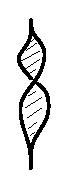
\includegraphics[height=3cm]{twist.eps}}} \quad = \quad \vcenter{\hbox{
\includegraphics[height=3cm]{invvh2.eps}}}.
\]
This suggests that we may represent framed links in $\Sigma \times I$ as link diagrams on $\Sigma$. Indeed, equivalence under ambient isotopy is captured by the Reidemeister moves 2, 3, and a modified Reidemeister move 1:

\[
    \vcenter{\hbox{
\includegraphics[height=3cm]{modifiedr1.eps}}} \quad = \quad \vcenter{\hbox{
\includegraphics[height=3cm]{modifiedr1resolution.eps}}}.
\]

\AP{Add pictures of RII and RIII for good measure.}
Below are some examples of framed tangle diagrams.

\[
    \vcenter{\hbox{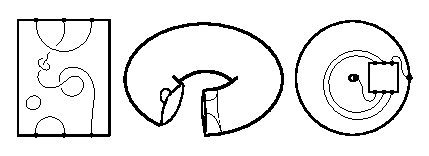
\includegraphics[height=3cm]{Ntangles.eps}}}
\]
\AP{fix torus picture by removing band.}

Define the \textbf{writhe} of a tangle diagram is the number of positive crossings minus the number of negative crossings. It is easy to see that the Reidemeister moves above preserve the writhe of a diagram, so the concept is well defined. Writhe should be thought of as a grading on the free $R$-module on the set of tangles in the given space, which provides a good reason to work with framed links over ordinary links. Such a module is a main ingredient of this theory, so let's honor it with a proper discussion.

\begin{definition}
Let $\ct(M, N)$ be the free $R$-module generated by the set of framed $N$-tangles in $M$. Analagously, we can define $\ct^{or}(M,N)$ to be the free $R$-module generated by the set of oriented framed $N$-tangles in $M$. All definitions which are to follow in this section have an analagous definition using oriented tangles. Also, we will formally define $\cs_R(\varnothing, \varnothing) := R$. 
\end{definition}

The construction $\ct( -, -)$ is actually a symmetric monoidal functor $\ct: \sfc \to R\textsf{-Mod}$ for a careful choice of category $\sfc$ which we now describe. The objects of $\sfc$ are pairs $(M, N)$ of the same type as discussed previously. A morphism $(f, W): (M', N') \to (M, N)$ is a pair of a smooth, orientation-preserving embedding $f: M' \to M$ such that $M - f(M')$ is either a smooth 3-manifold or the empty set, and choice of $W \in \ct\big( M-f(M'), N \sqcup f(N') \big)$ (unless $M - f(M')$ is empty, in which case $W$ is a formal symbol for the "empty link" in the empty set). Composition is given by $(g, W') \circ (f, W) = (g \circ f, W' \cup W)$, which is associative since $\circ$ and $\cup$ are associative.

\AP{Give a picture of composition in $\sfc$.}

The induced map denoted $W: \ct(M', N') \to \ct(M, N)$ is a linear map defined by $W(T) = W \cup T$, and we will refer to such a linear map $W$ as a \textbf{wiring}. We are abusing notation by denoting this linear map by $W$, but it should be clear from the context what $f$ is since it is technically encoded in the data of the element $W \in \ct\big( M-f(M'), N \sqcup f(N') \big)$. It is true that $\ct$ preserves composition and identity morphisms, making and so $\ct$ is functorial. $\sfc$ can now be equipped with a symmetric monoidal structure via disjoint union. It is clear that 
\[\ct_R(M \sqcup M', N \sqcup N') \cong \ct_R(M, N) \underset{R}{\otimes} \ct_R(M', N')\]
for any sets of framed points $N \subset \partial M$ and $N' \subset \partial M'$. The unit is given by the object $(\varnothing, \varnothing) \in \sfc$ and define $\ct(\varnothing, \varnothing) := R$, which makes $\ct$ a symmetric monoidal functor. 

\begin{definition}
Let $B$ be the smooth closed $3$-ball, $N_i$ be a choice of $2i$ boundary points of $B$, and let $X \subset \underset{i \in \N}{\bigsqcup} \ct(B, N_i)$ be some (typically finite) set, which we will call a set of \textbf{skein relations}. Given any tangle module $\ct(M, N_M)$, there exists a submodule $\ci(X)$ generated by the set 
\[\{ W(x) \mid x \in X \text{ and } W:\ct(B, N_B) \to \ct(M, N_M) \text{ is a wiring diagram} \}.\] 
A quotient of the form $\cs_X(M, N) := \ct(M, N) / \ci(X)$ is called a \textbf{skein module} of $M$ relative to $N$. If $N = \varnothing$ is the empty set, we may use the notation $\cs_X(M) := \cs_X(M, \varnothing)$. Similar definitions may be given using oriented and/or unframed tangles instead. 
\end{definition}
The construction $\cs_X(-, -)$ is a functor in the same way that $\ct(-, -)$ is; a smooth, orientation-preserving embedding $f: M \to M'$ and an element $W \in \cs_X\big( M-f(M'), N \sqcup f(N') \big)$ (assume $N$ is disjoint from $\im(f)$) defines a linear map $W: \cs_X(M, N) \to \cs_X(M', N')$. In fact, the quotient maps $\alpha_{(M, N)}: \ct(M, N) \to \cs_X(M, N)$ yield a natural transformation. In other words, given a morphism $(M, N) \to (M', N')$ in $\sfc$, the diagram
\begin{center}
\begin{tikzcd}
	\ct(M, N) \arrow[d,"\alpha_{(M, N)}"] \arrow[r, "W"] 
	& \ct(M', N') \arrow[d, "\alpha_{(M', N')}"]\\
	\cs_X(M, N) \arrow[r, "W"] & \cs_X(M', N')
\end{tikzcd}
\end{center}
commutes. Such a functor will be called a $\textbf{skein theory}$ (or \textit{oriented} skein theory if the skein relations are based on oriented tangles). 

For any oriented surface $\Sigma$, we can define a category $\sfskein_X(\Sigma)$ which we will call a $\textbf{skein category}$. The objects of this category are finite sets of framed points (together with a choice of orientation if the skein theory is oriented) $N$ in $\Sigma$, and the morphisms $N \to N'$ are elements of $\cs_X\big(\Sigma \times I, (N \times \{0\}) \sqcup (N' \times \{1\})\big)$, so the category is $R$-linear. Write composition of morphisms by concatenation. If $y:N \to N'$ and $z:N' \to N''$ are morphisms, then their composite $yz:N \to N''$ is constucted by gluing $y$ on top of $z$ through $N'$ and rescaling the interval coordinate appropriately.

\AP{Picture of composition in $\sfskein_X(\Sigma)$.}

The endomorphism algebras in this category are called \textbf{skein algebras} and are denoted by $\cs_X(\Sigma, N) := \cs_X(\Sigma \times I, (N \times \{0\}) \sqcup (N \times \{1\}) \big)$. If $N$ is the empty set, then we reduce the notation to simply $\cs_X(\Sigma)$.

If $f: \Sigma \to \Sigma'$ is a smooth embedding of surfaces, then there is an induced functor 
\[
\sfskein_X(f): \sfskein_X(\Sigma') \to \sfskein_X(\Sigma)
\]
defined on objects by $\sfskein_X(f)(N) = f(N)$ and on morphisms in the following way. First, extend $f$ trivially to $f \times \id_I: \Sigma \times I \to \Sigma' \times I$. Then, in the skein algebra of the complement of the image of $f \times \id_I$, choose the multiplicative identity element $e \in \cs_X\big( \Sigma' - \im(f) \big)$ which is the empty tangle. The pair $(f \times \id_I, e)$ is an object in the category $\sfc$, which gives rise to a wiring
\[e: \cs_X\Big(\Sigma \times I, \big(N \times \{0\}\big) \sqcup \big(N' \times \{1\}\big) \Big) \to \cs_X\Big(\Sigma' \times I, \big(f(N) \times \{0\}\big) \sqcup \big( f(N') \times \{1\} \big) \Big)\]
via the functor $\cs_X$. Now we may define what $\sfskein_X(f)$ does to morphisms: $\sfskein_X(f)(y) = e(y)$ for any $y \in \cs_X\Big(\Sigma \times I, (N \times \{0\}) \sqcup (N' \times \{1\}) \Big)$.

\AP{Picture of how $\sfskein_X(f)$ works on morphisms.}

It is clear that $\sfskein_X(f)$ preserves composition and identity morphisms. Therefore, if we let $\mathsf{Surf}$ be the category of smooth embeddings between smooth oriented surfaces, we can summarize our last few points by saying we have a functor
\[
\sfskein_X: \mathsf{Surf} \to \mathsf{Cat}.
\]
In particular, $\sfskein_X(f)$ defines algebra homomorphisms on the skein algebras
\[e: \cs_X\big(\Sigma, N\big) \to \cs_X\big(\Sigma', f(N)\big).\]
\AP{We use this type of algebra homomorphism when we embed the annulus into the torus.}

\begin{remark} \label{rem:skeinaction}
The above homomorphisms are a special case of a more general type of map. If $N$ is a set of framed points on $\Sigma$, then a smooth embedding $f: \Sigma \to \partial M$ induces a $\cs_X(\Sigma, N)$-module structure on $\cs_X\big(M, N'\big)$ for any $N'$ with $f(N) \subseteq N'$. The action is given by ``pushing tangles in through the boundary". In other words, the pre-composition of a smooth embedding of a collar neighborhood $g: \partial M \times I \to M$ with $f \times \id_I: \Sigma\times I \to \partial M \times I$ induces a bilinear map
\[
\cs_X(\Sigma, N) \times \cs_X(M, N') \to \cs_X(M, N')
\]
because $M$ minus a collar neighborhood is diffeomorphic to itself. Alternatively, a choice of element in $\cs_X(\Sigma, N')$ produces a wiring $\cs_X(M, N') \to \cs_X(M, N')$.

\AP{Picture of action.}
\end{remark}


\section{Examples of Skein Theories} \label{sec:skeintheories}

The last section leaves us with an important and unanswered question. Which sets of skein relations $X$ produce interesting skein theories? One class of examples is found by importing sets of relations satisfied by morphisms in a linear ribbon category as skein relations. Ribbon categories are braided monoidal categories which are rigid and equipped with a twist morphism for every object, satisfying some compatibility conditions. The axioms are such that the morphisms may be interpreted as framed braid diagrams. In particular, the morphisms satisfy the Reidemeister moves shown previously. We will discuss three examples of skein theories derived from skein relations which are meant to emulate linear relations satisfied by the braid and twist morphisms in certain ribbon categories coming from the representation theory of quantum groups, a topic which has generated a lot of interest from mathematicians since the 1980s. The categories of representations of quantum groups are ribbon categories with non-involutive braidings and the skein relations below capture how far off the braidings are from being involutive.  

Here, we are forced to fix a base ring. For our purposes, $R$ must be a commutative ring containing invertible elements $s$ and $v$. Typical choices of $R$ are $\Z[s^{\pm 1}, v^{\pm 1}], \Q(s, v)$, or some other ring in between these.  In particular, the theorem \AP{Cite BB} is stated over this ring, a result we will depend heavily on later on. \\

\begin{example}[\textit{Kauffman (Dubrovnik) Skein Relations}]
Let $X_1$ be the set of two unoriented skein relations
\begin{flalign*}
    (1) \quad \vcenter{\hbox{
\includegraphics{poscross.eps}}} &= \vcenter{\hbox{
\includegraphics{negcross.eps}}} + (s-s^{-1}) \,\, \vcenter{\hbox{
\includegraphics{idresolution.eps}}} - (s-s^{-1}) \,\, \vcenter{\hbox{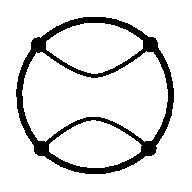
\includegraphics{capcupresolution.eps}}} \\ \\
    (2) \quad \vcenter{\hbox{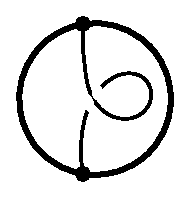
\includegraphics{vh.eps}}} &= v \,\, \vcenter{\hbox{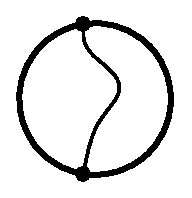
\includegraphics{frameresolution.eps}}}.
\end{flalign*}
The functor $\cd(-,-) := \cs_{X_1}(-,-)$ is the Dubrovnik skein theory (sometimes just called the Kauffman skein theory). We will use the notation $\mathsf{D}(-) := \sfskein_{X_1}(-)$ for the Dubrovnik skein categories. Using the Dubrovnik variant is important for us (see \AP{universal enveloping algebra result}). This theory is related to Dubrovnik polynomials in that the Dubrovnik polynomial of a link is a normalized value of the link in $\cd(S^3)$. The normalization is often so that the Dubrovnik polynomial of the unknot is $1$, whereas the value of the unknot in $\cd(S^3)$ is $\delta_\cd := 1 - \frac{v-v^{-1}}{s-s^{-1}}$, which can be deduced from the skein relations.
\end{example}

\begin{example}[\textit{HOMFLYPT Skein Relations}]
Next, let $X_2$ be the set of two oriented skein relations
\begin{flalign*}
    (1) \quad \vcenter{\hbox{
\includegraphics{poscrossor.eps}}} &= \vcenter{\hbox{
\includegraphics{negcrossor.eps}}} + (s-s^{-1}) \,\, \vcenter{\hbox{
\includegraphics{idresolutionor.eps}}} \\ \\
    (2) \quad \vcenter{\hbox{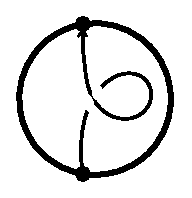
\includegraphics{vhor.eps}}} &= v \,\, \vcenter{\hbox{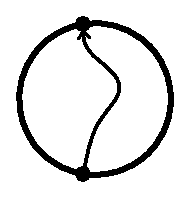
\includegraphics{frameresolutionor.eps}}}.
\end{flalign*}
The functor $\ch(-,-) := \cs_{X_2}(-,-)$ is the HOMFLYPT skein theory and we use the notation $\mathsf{H}(-) := \sfskein_{X_2}(-)$ for the HOMFLYPT skein categories. As in the Dubrovnik case, this theory is related to HOMFLYPT polynomials so that the HOMFLYPT polynomial of a link is a normalized value of the link in $\ch(S^3)$. Again, some often make the choice to normalize this polynomial so that the value of the unknot is $1$, but the value of the unknot in $\ch(S^3)$ is $\delta_\ch := -\frac{v-v^{-1}}{s-s^{-1}}$.
\end{example}

\begin{example}[\textit{Kauffman Bracket Skein Relations}]
As a final example, let $X_3$ be the set of two unoriented skein relations
\begin{flalign*}
    (1) \quad \vcenter{\hbox{
\includegraphics{poscross.eps}}} &= s \,\, \vcenter{\hbox{
\includegraphics{idresolution.eps}}} + s^{-1} \,\, \vcenter{\hbox{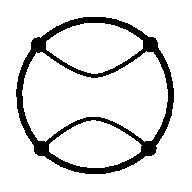
\includegraphics{capcupresolution.eps}}} \\ \\
    (2) \quad \vcenter{\hbox{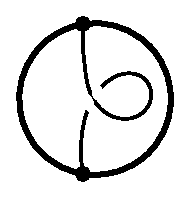
\includegraphics{vh.eps}}} &= -s^{-3} \,\, \vcenter{\hbox{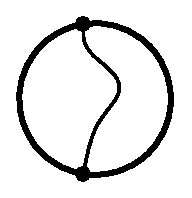
\includegraphics{frameresolution.eps}}}.
\end{flalign*}
The functor $\ck(-,-) := \cs_{X_3}(-,-)$ is the Kauffman bracket skein theory (not be confused with the Kauffman skein theory) and we use $\mathsf{K}(-) := \sfskein_{X_3}(-)$ to notate the Kauffman bracket skein categories. The value of a link in $\ck(S^3)$ is equal to its bracket polynomial, which may be normalized as above to obtain its Jones polynomial. One could choose the framing parameter to be $v$ instead of $-s^{-3}$ like we did before without any obvious consequences, but it is standard in the literature to make the choice we present here.  
\end{example}

\begin{remark}
Any linear combination of tangles which satisfy the Dubrovnik skein relations will also satisfy the Kauffman bracket skein relations after making the specialization $v=-s^{-3}$. This can be seen by performing the calculation in the relative skein algebra of the ball with $4$ points. Let $\sigma^\pm$ be the diagrams of positive and negative crossings, $e$ the planar diagram with two vertical strands, and $c$ the planar diagram with two horizontal strands. Then the Dubrovnik skein relation is
\[
\sigma^+_\cd - \sigma^-_\cd - (s-s^{-1})e_\cd + (s-s^{-1})c_\cd = 0
\]
and the Kauffman bracket skein relation implies
\begin{align*}
\sigma^+_\ck &= se_\ck + s^{-1}c_\ck \\
\sigma^-_\ck &= sc_\ck + s^{-1}e_\ck
\end{align*}
where the subscript indicates which skein module the diagrams are in. Consider the assignment $d_\cd \mapsto d_\ch$ for any tangle $d$ in the ball relative to those $4$ points. Then observe:
\begin{eqnarray*}
& &\sigma^+_\ck - \sigma^-_\ck - (s-s^{-1})e_\ck + (s-s^{-1})c_\ck \\
=& &(se_\ck + s^{-1}c_\ck) - (sc_\ck + s^{-1}e_\ck) - (s-s^{-1})e_\ck + (s-s^{-1})c_\ck \\
=& &0
\end{eqnarray*}

Therefore, there is a natural transformation of skein theories 
\[
\eta: \cd(-,-) \to \ck(-,-)
\] 
whose components are essentially the identity map, using the same type of assignment as we did above. Note that any component of $\eta$ corresponding to a skein algebra is an algebra homomorphism since the map preserves the (topological) product structure of the manifold.
\end{remark}

In this work, we will be focused on generalizing existing results from the HOMFLYPT and Kauffman bracket skein theories to the Dubrovnik skein theory, but we will state a few facts regarding the HOMFLYPT and Kauffman bracket skein theories when it is valuable for us to do so. 

\AP{Maybe add a remark about Turaev's work on deformations of the Goldman Lie algebras? Could potentially say a lot to motivate the topic, but I'm not super familiar with a lot of it.}

\AP{Add comments about the Dubrovnik and HOMFLYPT skein algebras being graded by ther fundamental group of the surface.}

\section{Skein Algebras of Tangles in a Cube} \label{sec:cube}

In the case where $\Sigma = I \times I$, the endomorphism objects of $\mathsf{D}(I \times I), \mathsf{H}(I \times I)$, and $\mathsf{K}(I \times I)$ are known and provide the motivation for why the choices of skein relations are what they are. For an integer $n \geq 1$, let $[n]$ be a set of $n$ points in $I \times I$, chosen to be evenly spaced along the line segment $\{ 1/2 \} \times I$ (choose so that all points share the same orientation if in the context of an oriented skein theory). Then the endomorphism algebras 
\[
BMW_n := \End_\mathsf{D}(I \times I)([n]), \qquad H_n := \End_\mathsf{H}(I \times I)([n]), \qquad TL_n := \End_\mathsf{K}(I \times I)([n])
\]
are known to be isomorphic to the Birman-Murakami-Wenzl, (Type A) Hecke, and Temperley-Lieb algebras, respectively (\AP{*Add citations}). 

Let $q \in \C$ be not a root of unity, $U_q(\mathfrak{gl}_N)$ be the Drinfeld-Jimbo quantum group associated to the Lie algebra $\mathfrak{gl}_N$, and $V$ be the natural representation of $U_q(\mathfrak{gl}_N)$ (\AP{cite Chari-Pressley book}). Then $H_n$ acts on the $n$-fold tensor product $V^{\otimes n}$ by $U_q(\mathfrak{gl}_N)$-linear endomorphisms, and this action generates $\End_{U_q(\mathfrak{gl}_N)}(V^{\otimes n})$. This is actually part of the statement of quantum Frobenius-Schur-Weyl duality: $V^{\otimes n}$ is a $U_q(\mathfrak{gl}_N)$-$H_n$-bimodule, and the action of one algebra generates the linear endomorphisms with respect to the other. So a representation of one algebra determines a representation of the other via tensor product with $V^{\otimes n}$. The Birman-Murakami-Wenzl algebra plays the role of the Hecke algebra for $U_q(\mathfrak{g}_N)$ in the case where $\mathfrak{g}$ is one of the orthogonal or symplectic Lie algebras. For this reason, from a Lie theoretic point of view, the HOMFLYPT skein theory is thought of as a ``type A" theory, while the Dubrovnik skein theory is a ``types B, C, D" skein theory.

As for the Temperley-Lieb algebra $TL_n$, it acts on the $n$-fold tensor power $V^{\otimes n}$ of the natural representation of $U_q(\mathfrak{gl}_2)$. Actually, there is a surjective algebra homomorphism $\pi_{TL}: H_n \to TL_n$ and the action $H_n \to \End_{U_q(\mathfrak{gl}_2)}(V^{\otimes n})$ factors through this homomorphism (see \AP{cite Jimbo}). One can conclude that the action of $H_n$ on $V^{\otimes n}$ is not faithful, at least in the case when $N=2$ and $n \geq 2$. \AP{sl2 vs gl2?}

Much is known about these algebras and some of the results surrounding them are very useful in our context. One of the main ideas is that each of the algebras discussed above has a family of idempotents which provide algebraically nice closures to links in the skein algebra of an annulus. Let's first describe the Hecke algebra in more detail before focusing on the BMW algebra. 

For any partition $\lambda$ of $n$, there exists an element $y_\lambda \in H_n$ which is idempotent, so that $y_\lambda^2 = y_\lambda$, and minimal in the sense that it generates a minimal left-ideal of $H_n$ (see \AP{cite Aiston-Morton}). The elements $y_n := y_{(n)}$ corresponding to single row partitions are called \textbf{(Hecke) symmetrizers}. These elements have a certain absorption property which makes them unique, which we will now describe. Let us use $\sigma_i \in H_n$ be the positive crossing between the $i^{\rm{th}}$ and $(i+1)^{\rm{th}}$ strands. 
\AP{Picture of oriented $\sigma_i \in H_n$.}
The algebra $H_n$ is generated by the $\sigma_i$ and the symmetrizers are the unique idempotent elements satisfying $\sigma_i y_n = s y_n = y_n \sigma_i$. In this way, $y_n$ corresponds to a $1$-dimensional representation of $H_n$ (it is a deformation of the trivial representation of $\C S_n$ where $s=1$).

A similar story holds for the BMW algebra. Firstly, $BMW_n$ is generated by positive crossing elements $\sigma_i$ and cap-cup elements $c_i$. 
\AP{pictures of $\sigma_i$ and $c_i$}
The $c_i$ generate a proper ideal $I_n$ in $BMW_n$. In (\AP{cite BB}), the authors show that the complement of $I_n$ in $BMW_n$ is isomorphic to $H_n$, giving an isomorphism $BMW_n \cong H_n \oplus I_n$. Then they construct an additive and multiplicative (but non-unital) homomorphism 
\begin{equation}
\Gamma_n : H_n \to BMW_n
\end{equation}
which is a section of the natural projection $BMW_n \to H_n$ such that 
\begin{equation} \label{eq:bbsectionproperty}
\Gamma_n(x)y = 0 = y \Gamma_n(x) \quad \textrm{for } x \in H_n, y \in I_n.
\end{equation}
Using this section, one can transport the minimal idempotents $y_\lambda \in H_n$ to minimal idempotents $\tilde{y}_\lambda := \Gamma_n(y_\lambda) \in BMW_n$. The elements $\tilde{y}_n := \tilde{y}_{(n)}$ are called the \textbf{(BMW) symmetrizers} and are the unique idempotent elements of $BMW_n$ satisfying the properties of the Hecke symmetrizers and property \eqref{eq:bbsectionproperty}. By \AP{cite Shelly}, these symmetrizers satisfy a very useful recurrence relation
\begin{equation} \label{eq:shellyrecurrence}
*=*
\end{equation}
\AP{Change $f_n$ to $\tilde{y}_n$ in symmetrizer pictures.}
\AP{Define quantum integers and $\beta_n$}
%\[
%[n+1] \vcenter{\hbox{\includegraphics[width=2.9cm]{f_nplus1.eps}}} = [n]s^{-1} \vcenter{\hbox{\includegraphics[width=2.9cm]{f_notimes11otimesf_n.eps}}} + \vcenter{\hbox{\includegraphics[width=2.9cm]{sigma_ndotssigma_11otimesf_n.eps}}} + [n]s^{-1} \beta_n \vcenter{\hbox{\includegraphics[width=2.9cm]{f_notimes1H1otimesf_n.eps}}}.
%\]
For what it's worth, this relation descends to a well-known recurrence relation for the $y_n \in H_n$ via the projection map described above ($\tilde{y}_n$ gets sent to $y_n$ and the last diagram on the right-hand side gets sent to $0$). 

\AP{Come back and add braiding/twist identities from BB if we need them.}

\AP{Would it be wise to include the BB matrix algebra description of $BMW_n$? Might be useful to point out the central idempotents $z_\lambda$, which are distinct from the $y_\lambda$, even though I don't think I use them anywhere. Maybe a quick remark would suffice. Note that the annular closure of the $y_\lambda$ is equal to the annular closure of $z_\lambda$.}

\section{Skein Algebras of the Annulus} \label{sub:annulus}

Let's use the notation $A := S^1 \times [0,1]$ for the annulus. The thickened annulus represents perhaps the simplest space with non-trivial topology that can harbor links. There are often many different smooth embeddings of the thickened annulus into a given 3-manifold $M$ (one for every element of $\pi_1(M)$, at the very least). Keep in mind that if we have a smooth embedding $f: A \times I \hookrightarrow M$, then we have an induced linear map between skein modules $\cs_X(f): \cs_X (A) \to \cs_X (M)$, allowing us to prod for information about $\cs_X(M)$. One useful type of embedding of $A$ is into a tubular neighborhood of a knot, which is often called \textit{decorating} or \textit{threading} a knot.

A first observation is that any skein algebra of the form $\cs_X(A)$ is commutative because the link algebra $\cs_\varnothing(A)$ is a commutative algebra. To see this, consider the product of two links $L_1$ and $L_2$ in the link algebra and start by stretching $L_2$ towards the outer boundary past $L_1$, followed by moving it down below the furthest point of $L_1$, and finally contracting $L_2$ can to its original radial position. This is essentially the Eckmann-Hilton argument. 

We'll tackle describing the structure of $\ck(A)$ before the others since it is the easiest. The Kauffman bracket skein relation allows one to resolve all crossings in any diagram on any surface $\Sigma$. It is a theorem of Pzytycki that the set of non-trivial mutli-curves (non-trivial meaning that no curve bounds a disk), together with the empty link in $A \times \{ \ast \}$ forms a basis of $\ck(A)$ (actually, the theorem is stated for any skein algebra, see \AP{cite}). There is only one non-trivial curve $z$ and the set $\{ z^k \}_{k \in \N}$ exhaust all of the multicurves. Therefore, $\ck(A)$ is a polynomial algebra $R[z]$. 

The HOMFLYPT and Dubrovnik cases are more complicated because the skein relations do not allow one to resolve all the crossings in a diagram. However, they do allow one to change a diagram with a negative crossing into a diagram with a positive crossing, plus diagrams with a lesser number of crossings. It follows that the skein algebras $\ch(A)$ and $\cd(A)$ are generated by knots with only positive crossings. Let $z_i$ be a knot in $A$ with winding number $i$ around the annulus. Turaev shows in \AP{cite} that the $z_i$ are algebraically independent by showing their HOMFLYPT and Dubrovnik polynomials are algebraically independent. Therefore, $\ch(A)$ is a polynomial algebra $R[z_i, i \in \Z_{\neq 0}]$. $\cd(A)$ has half as many generators since the $z_i$ in that setting are unoriented, but $\cd(A)$ is a polynomial algebra $R[z_i, i \in \Z_{> 0}]$ by the same arguments. 

\AP{Picture of $z_i$}

The skein algebras of tangles in a cube relate to the skein algebras of the annulus via a map $\cl(-)$, depicted as a wiring diagram below. 

\AP{Picture of closure}

Let $\widetilde{Q}_\lambda := \cl(\tilde{y}_\lambda) \in \cd(A)$. Zhong and Lu show in \AP{cite} that the set $\{ \widetilde{Q}_\lambda \}_\lambda$ forms a basis of $\cd(A)$ over the base ring $R=\Q(s, v)$, where $\lambda$ ranges over all paritions. Actually, it is an eigenbasis with respect to the meridian map
\AP{picture of meridian map.}
where the eigenvalue of $Q_\lambda$ is 
\[
c_\lambda = \delta_\cd + ( s - s^{-1} ) \sum_{\square \in \lambda} v^{-1} s^{2 \textrm{cn}(\square)} - v s^{-2 \textrm{cn}(\square)}
\]
and where $\textrm{cn}(\square) := j - i$ is the \textit{content} of the box in the $\square$ in $i^\textrm{th}$ row and $j^\textrm{th}$ column of the Young diagram of the partition $\lambda$. Two distinct partitions $\lambda$ and $\lambda '$ give rise to distinct values of $c_\lambda$ and $c_\lambda'$. Therefore, each of the eigenspaces is $1$-dimensional. 

The behavior of $\widetilde{Q}_\lambda$ is similar to that of the $Q_\lambda := \cl^+(y_\lambda) \in \ch(A)$ where $\cl^+(-)$ is defined by orienting the strands in wiring digram of $\cl(-)$ counter-clockwise. Using the description $\ch(A) = R[z_i, i \in \Z_{\neq 0}]$, consider the subalgebras $\ch(A)^+ := R[z_i, i \in \Z_{> 0}]$ and $\ch(A)^- := R[z_i, i \in \Z_{< 0}]$. Then the two subalgebras are isomorphic via the linear involution defined by $z_i \mapsto z_{-i}$ and $\ch(A) \cong \ch(A)^+ \otimes \ch(A)^-$. The $\{ Q_\lambda \}_\lambda$ forms an eigenbasis of $\ch(A)^+$ with resepect to the meridian map and the eigenspaces are $1$-dimensional. As a side remark, the linear involution $z_i \mapsto z_{-i}$ may be realized topologically by rotating the thickened annulus $\pi$ radians around an appropriately centered axis parallel to $A$ and taking the induced skein map. We will call this map the \textit{flip map}.

In \AP{cite Lukac}, it's shown how to interpret $\ch(A)^+$ as the ring of symmetric functions $\Lambda$ (also see \AP{cite Morton Murphy Operators}). There is an injective algebra homomorphism $\Lambda \to \ch(A)^+$ which sends the Schur function $s_\lambda$ to the minimal idempotent closure $Q_\lambda$. This theorem has plenty of implications. For example, the structure constants of $\Lambda$ in the basis $\{ s_\lambda \}_\lambda$ are the Littlewood-Richardson coefficients, which are then sent to structure constants of $\ch(A)^+$ in the basis $\{ Q_\lambda \}_\lambda$. In Chapter \AP{reference}, we discuss partial results surrounding the Dubrovnik analogue of this homomorphism. See Section \AP{reference} for a summary about the ring $\Lambda$.

Another application of the interpretation of $\ch(A)^+$ as $\Lambda$ is the definition of new special links in the skein algebra. There is a family of elements in $\Lambda$ known as the power sum symmetric functions, whose counterparts in $\ch(A)^+$ we will denote by $P_k$ for integers $k \geq 1$. These elements are algebraically independent in $\Lambda_\Q := \Q \otimes \Lambda$. Therefore, ordered monomials in the $P_k$ form a basis of $\ch(A)^+$.


\section{Skein Algebras of the Torus}

The power sum elements $P_k$ described above are known to behave wonderfully in skein theoretic computations. This allows for a simple description of the HOMFLYPT skein algebra of the torus $\ch(T^2)$ in terms of generators and relations. First, let's define the generators. Given an $r$ which is either a rational number, or $\pm \infty$, there is an oriented smooth embedding 
\[
\iota_{r}: A \hookrightarrow T^2
\]
of the annulus into a tubular neighborhood of the line of slope $r$ in the flat torus. Consider the embeddings $\iota_{r}$ and $\iota_{-r}$ to be the same embedding with opposite orientations. Now $\iota_r$ induces an algebra homomorphism
\[
\ch(\iota_r): \ch(A) \to \ch(T^2)
\]
on the level of skein algebras. The $\iota_r$ are distinct isotopically (even homotopically) and are exhaustive in the sense that any knot in the thickened torus is may be represented as being contained in the image of an $\iota_q$. Therefore, any basis of $\ch(A)^+$ defines a basis of $\ch(T^2)$. Let's consider this with respect to the the power-sum monomial basis of $\ch(A)^+$. More precisely, for any pair of integers $\xx = (a, b)$ where $k = \gcd(\xx)$, define 
\[
P_\xx := \ch(\iota_{a/b})(P_k).
\]

In \AP{cite MS}, Morton and Samuelson prove that the skein algebra $\ch(T^2)$ admits a presentation with generators the elements of $\{ P_\xx \mid \xx \in \Z^2 \}$, subject to the single family of relations 
\[
[P_\xx, P_\yy] = \big( s^{\det(\xx,\yy)} - s^{-\det(\xx,\yy)} \big) P_{\xx + \yy}.
\]
This presentation exhibits a relationship to the elliptic Hall algebra: a 2-parameter family of algebras obtained via Hall algebra decategorification of categories of coherent sheaves over certain elliptic curves (see \AP{Burban-Schiffman}). Along the diagonal of the parameter space, the Burban-Schiffman presentation of the elliptic Hall algebra matches the Morton-Samuelson presentation of the skein algebra of the torus. At the very least, this highlights two things. Firstly, the skein algebra of the torus admits a known deformation. Secondly, skein algebras are connected to surprising areas of mathematics and hence deserve our attention. \AP{Is this paragraph correct?}

Next we describe the Kauffman bracket skein algebra of the torus, although the order of exposition is opposite to the historical order of discovery. The story is actually quite similar to the HOMFLYPT case. Recall that $\ck(A)$ is a polynomial algebra $R[z]$ where $z$ is the simple closed curve around the hole of the annulus with winding number $1$. There exist polynomials known as \textit{Chebyshev polynomials} $T_k \in R[z]$ for all integer $k \geq 1$ which form a basis of $\ck(A)$. For any pair of integers $\xx = (a, b) \in \Z^2$, define elements $T_\xx \in \ck(T^2)$ as 
\[
T_\xx := \ck(\iota_{a/b})(T_k).
\]
Note that $T_\xx = T_{-\xx}$ because the $T_k$ are fixed under the flip map, which is possible since the Kauffman bracket skein theory is an unoriented skein theory. With this in mind, we may pass to the smaller indexing set $Z^2 / \langle \xx = -\xx \rangle$. Using these elements, Frohman and Gelca \AP{cite} prove that the skein algebra $\ck(T^2)$ admits a presentation with generators $T_\xx$ subject to the relations
\[
T_\xx T_\yy = s^{\det(\xx, \yy)} T_{\xx + \yy} + s^{-\det(\xx, \yy)} T_{\xx - \yy}
\]
which the authors call the ``product-to-sum" formulas. There is an algebra called the \textit{noncommutative torus}, which is a one-parameter deformation of the algebra of continuous functions on the torus. The Frohman-Gelca presentation of $\ck(T^2)$ matches a presentation of the invariant subalgebra of the noncommutative torus with respect to a certain involutive action, as shown in \AP{cite FG}. \AP{Is this paragraph correct?}

Given the similarity between the presentations of $\ch(T^2)$ and $\ck(T^2)$, one might suspect that there exists a similar description of the Dubrovnik skein algebra $\cd(T^2)$. The answer to this question is affirmative, which is what we discuss in Chapter \AP{How to reference a chapter?}


\section{A Relative Skein Algebra of the Annulus} \label{sec:relativeannulus}

At this point in the story we have introduced special links in the skein algebras of the annulus and described how we can transport these into other skein modules via threading knots. In order to say anything meaningful about these threadings, we ought to know how these special links will interact with other links once in the resulting space. For example, is there an easy way to describe how can we pass a special link through a single strand of another link? To answer this question universally, we should answer it in a certain relative skein algebra which is the endomorphism algebra of one point in the skein category of the annulus. Appropriate wirings from this skein algebra into other skein modules will give us our desired description. Here we will describe this algebra in more detail and summarize what is already known. 

First we will restrict ourselves to the HOMFLYPT case, for which we summarize the results from \AP{Morton, Murphy operators}. The object we would like to discuss is $\ca_\ch := \ch(A, [1])$, which is depicted diagramatically as an annulus with one point on each boundary component. This algebra is closely related to the affine Hecke algebra of type A, $\dot{H}_1$ (see \AP{cite MS}). Two of the most basic elements of $\ca_\ch$ are
\AP{Pictures of identity $e$ and once around counter-clockwise $a$.}
The product in the algebra in this digrammatic notation is given by nesting annuli. 

Let $\cc_\ch := \ch(A)$. Then, $\cc_\ch$ admits both a left $\cc_\ch$-action by pushing links infront of tangles in $\ca_\ch$.
\AP{Picture of left action.}
It is known that there is an equality of algebras between $\ca_\ch$ and the Laurent polynomial algebra $\cc_\ch[a, a^{-1}]$. In particular, $\ca_\ch$ is commutative and the left action is determined by how it acts on $e$.

Analagously, there is a right $\cc_\ch$-action by pulling links in behind tangles in $\ca_\ch$. 
\AP{picture of right action.}
Both actions are examples of those arising from embeddings into the boundary of the thickened annulus, as described in Remark \ref{rem:skeinaction}. The left and right actions obviously commute, endowing $\ca_\ch$ with a $\cc_\ch$-$\cc_\ch$-bimodule structure. It is probably worth pointing out that the left action is not equal to the right action. A simple measurement of how far off the two actions are from being equal would answer our question posed above. The answer is given as a commutator relation 
\begin{equation} \label{eq:pkcommutator}
e \cdot P_k - P_k \cdot e = (s^k - s^{-k}) a^k.
\end{equation}
\AP{Make sure this order is correct.}
The proof involves the definition of a certain wiring diagram, defining a linear map $H_n \to \ca_\ch$. The idempotents $y_{n}$ satisfy a certain recurrence relation, and the commutator relation above follows from writing $P_k$ in terms of the $y_n$ and calculations involving the image of this recurrence relation.

Eventually we would like to prove a Dubrovnik analogue of Equation \eqref{eq:pkcommutator} (see Section \ref{sec:commurationrelations}), but we still haven't defined any Dubrovnik analogue of the $P_k$ (see \AP{ref}). Nevertheless, we can discuss some of what was previously known about the algebra $\ca_\cd := \cd(A, [1])$ (see \AP{Shelly} for more details).

Let $\cc_\cd := \cd(A)$ and let $a, e \in \ca_\cd$ be the unoriented versions of the elements of the same name above. As in the HOMFLYPT case, there is a left-$\cc_\cd$ action on $\ca_\cd$ and the algebra $\ca_\cd$ is equal to the Laurent polynomial algebra $\cc_\cd[a^{\pm 1}]$. There is also a right-$\cc_\cd$ action on $\ca_\cd$, endowing $\ca_\cd$ with a bimodule structure. 

Consider the wiring diagrams
\AP{pictures of wirings. I would drop the subscript on $W_n$ for brevity and rename $\widetilde{W}$ to $W^*$ to not confuse with $\tilde{y}_n$.}
which define linear maps $BMW_n \to \ca_\cd$. Let $W_n := W(\tilde{y}_{n+1})$ and $W^*_n :=  W^*(\tilde{y}_{n+1})$ where the subscript denotes the ``winding number'' around $A$. Taking the image of Equation \eqref{eq:shellyrecurrence} under $W$ gives a relation
\begin{equation} \label{eq:recursionina1}
[n+1] W_n = e \cdot \tilde{h}_n + [n] s^{-1} a W_{n-1} + [n] s^{-1} \beta_n a^{-1} W^*_{n-1}
\end{equation}
where $\tilde{h}_n := \tilde{Q}_{(n)}$ is the annular closure of the symmetrizer $\tilde{y}_n$.

There are maps
\[
	(-)^*: BMW_n \to BMW_n \qquad \overline{(-)}: BMW_n \to BMW_n
\]
induced by the diffeomorphisms of the thickened square $(x, y, t) \mapsto (x, 1-y, 1-t)$ and $(x, y, t) \mapsto (x, y, 1-t)$, respectively. The map $\overline{(-)}$ is often called the \emph{mirror map} and is an $R$-anti-linear involution, while $(-)^*$ will be called the \emph{flip map} and is an $R$-linear involution. The symmetrizers $\tilde{y}_n$ are fixed under these maps because the mirror and flip maps preserve the properties which make $\tilde{y}_n$ unique.
Using the quotient map defined by the equivalence relation $(x, 0, t) \sim (x, 1, t)$, we may analagously define maps
\[
	(-)^*: \ca_\cd \to \ca_\cd, \qquad \overline{(-)}: \ca_\cd \to \ca_\cd
\]
which are linear and anti-linear involutions, respectively. We will also call these the flip map and the mirror map; it will be clear from the context which is being applied. These maps satisfy the relations
\begin{align*}
	\left( W \left( x \right) \right)^* &= W^* \left( x^* \right), & (y \cdot e)^* &= e \cdot y^*, \\
	\overline{W \left( x \right)} &= W \left( \overline{x} \right), & \overline{(y \cdot e)} &= e \cdot \overline{y}
\end{align*}
for any $x \in BMW_n$ or $y \in \cc_\cd$. Apply the flip, the mirror, and the composite of the two separately to Equation \eqref{eq:recursionina1} to obtain alternate versions of the original recurrence relation:
\begin{align} 
[n+1] W^*_n = \tilde{h}_n \cdot e + [n] s^{-1} a W^*_{n-1} + [n] s^{-1} \beta_n a W_{n-1} \label{eq:recursionina2}, \\
[n+1] W_n = \tilde{h}_n \cdot e + [n] s a W_{n-1} + [n] s \bar{\beta}_n a^{-1} W^*_{n-1} \label{eq:recursionina3}, \\
\quad [n+1] W^*_n = e \cdot \tilde{h}_n + [n] s a^{-1} W^*_{n-1} + [n] s^{-1} \bar{\beta}_n a W_{n-1}. \label{eq:recursionina4}
\end{align}

Rearranging the difference of Equations \eqref{eq:recursionina1} and \eqref{eq:recursionina2} gives a relation
\begin{equation}
\tilde{h}_n \cdot e - e \cdot \tilde{h}_n = \{n\} (a^{-1} W^*_{n-1} - a W_{n-1})
\end{equation}
which Shelly calls a \textit{fundamental skein relation} in $\ca_\cd$ since it reduces to to usual Dubrovnik skein relation when $n=1$. \AP{This might also be true in another sense, since there might be some connection between the wiring $W$ and something called the ``tube algebra", as pointed out by Henry Tucker.} In Chapter \AP{??}, we will provide a similar relation which amounts to rewriting the right-hand side of the equation in terms of elements of the form $h_i \cdot a^k$ (alternatively $a^k \cdot h_i$). 





\chapter{The Skein Algebra of the Torus}

\AP{Add some introduction and remark about collaboration.}


\section{Power Sum Elements}

Recall that there is a injective algebra homomorphism $\Lambda \to \ch(A)^+$ which sends the Schur function $s_\lambda$ to the minimal idempotent closure $Q_\lambda$. Use $h_n := Q_{(n)}$ to denote the image of the $n^\textrm{th}$ complete homogeneous symmetric function under this homomorphism. In \AP{MS} the authors import power sum elements from $\Lambda$ to $P_k \in \ch(A)$. The power sum elements have a concrete definition in $\Lambda$, but alternatively they may be defined using an equation of formal power series in the ring $\ch(A)[[t]]$ as
\begin{equation}
\sum_{k=1}^\infty \frac{P_k}{k} t^k = \ln \Bigg( 1 + \sum_{n=1}^\infty h_n t^n \Bigg)
\end{equation}
which writes each $P_k$ in terms of the generators $h_n$. 

Using the Beliakova-Blanchet section $\Gamma: H_n \to BMW_n$, we may emulate this definition to define ``power sum" elements $\tilde{P}_k \in \cd(A)$ by the formal power series equation
\begin{equation}
\sum_{k=1}^\infty \frac{\tilde{P}_k}{k} t^k = \ln \Bigg( 1 + \sum_{n=1}^\infty \tilde{h}_n t^n \Bigg)
\end{equation}
where $\tilde{h}_n := \tilde{Q}_{(n)}$ is the annular closure of the BMW symmetrizers $\tilde{y}_n = \Gamma(y_n)$.

Let's now continue our discussion of Section \ref{sec:relativeannulus} with the following theorem.

\begin{theorem} \label{thm:powersumcommutator}
For any $k \geq 1$, the relation
\begin{equation} \label{eq:powersumcommutator}
e \cdot \tilde{P}_k - \tilde{P}_k \cdot e = (s^k - s^{-k}) (a^k - a^{-k})
\end{equation}
holds. Equivalently,
\begin{equation}
a^i \cdot \tilde{P}_k - \tilde{P}_k \cdot a^i = (s^k - s^{-k}) (a^{k+i} - a^{-k+i})
\end{equation}
for any integer $i$.
\end{theorem}

We will split the proof of this theorem into two technical lemmas.

\begin{lemma} \label{lem:powersumcommutator1}
The relations of Theorem \ref{thm:powersumcommutator} hold if and only if 
\begin{equation} \label{eq:skewcommutator}
e \cdot (\tilde{h}_{n+2} + \tilde{h}_n) - (\tilde{h}_{n+2} + \tilde{h}_n) \cdot e = (sa + s^{-1}a^{-1}) (e \cdot \tilde{h}_{n+1}) - (s^{-1}a + sa^{-1}) (\tilde{h}_{n+1} \cdot e)
\end{equation}
for all integers $n \geq -1$, where $\tilde{h}_0 := 1$ and $\tilde{h}_{-1} := 0$.
\end{lemma}
\begin{proof}
The relations of Theorem \ref{thm:powersumcommutator} may be organized into a single power series equation
\begin{equation} \label{eq:skewcommutator}
\sum_{k=1}^\infty \frac{e \cdot \tilde{P}_k - \tilde{P}_k \cdot e}{k} t^k = \sum_{k=1}^{\infty} \frac {(s^k - s^{-k}) (a^k - a^{-k})}{k} t^k
\end{equation}
in $\ca_\cd [[t]]$. Rewrite this equation as
\begin{equation} \label{eq:powersumcommutator2} 
e \cdot \Bigg( \sum_{k=1}^\infty \tilde{P}_k \Bigg) - \Bigg( \sum_{k=1}^\infty \tilde{P}_k \Bigg) \cdot e = \sum_{k=1}^{\infty} \frac {(sat)^k}{k} + \sum_{k=1}^{\infty} \frac {(s^{-1}a^{-1}t)^k}{k} - \sum_{k=1}^{\infty} \frac {(s^{-1}at)^k}{k} - \sum_{k=1}^{\infty} \frac {(sa^{-1}t)^k}{k}
\end{equation}
We can make sense of the left-hand side by extending the algebra homomorphism $x \mapsto e \cdot (x)$ to an algebra homomorphism of rings of formal power series
\begin{center}
\begin{tikzcd}
\cd(A) \arrow[r, "e \cdot (-)"] \arrow[d, hook] & \ca_\cd \arrow[d, hook] \\
\cd(A)[[t]] \arrow[r, "e \cdot (-)"] & \ca_\cd[[t]]
\end{tikzcd}
\end{center}
and similarly for $(-) \cdot e$. Now for shorthand, define 
\[
H(t) := 1 + \sum_{n=1}^\infty \tilde{h}_n t^n
\]
and recall the Taylor series expansion
\[
-\ln(1-x) = \sum_{k=1}^\infty \frac{x^k}{k}
\]
which is a variation of the Newton-Mercator series. Then the Equation \eqref{eq:skewcommutator} becomes
\begin{equation} \label{eq:powersumcommutator3} 
e \cdot \Big( \ln\big(H(t)\big) \Big) - \Big( \ln \big(H(t)\big) \Big) \cdot e = - \ln(1 - sat) - \ln(1 - s^{-1}a^{-1}t) + \ln(1 - s^{-1}at) + \ln(1 - sa^{-1}t).
\end{equation}
The maps $e \cdot (-)$ and $(-) \cdot e$ commute with the natural logarithm. Use this and other natural log properties to write
\begin{equation}
\ln\Big( e \cdot \big( H(t) \big) \big( 1 - (sa + s^{-1}a^{-1})t + t^2 \big) \Big) = \ln\Big( \big( H(t) \big) \cdot e \big( 1 - (s^{-1}a + sa^{-1})t + t^2 \big) \Big).
\end{equation}
Exponentiating both sides and equating coefficients gives the system of equations defined in the statement of the lemma. Each step of the proof is invertible, and thus the two sets of relations are logically equivalent.
\end{proof}

\begin{lemma}
The relations of Lemma \ref{lem:powersumcommutator1} hold.
\end{lemma}
\begin{proof}
If $n=-1$, the relation we would like to show becomes 
\begin{equation*}
e \cdot \tilde{h}_1 - \tilde{h}_1 \cdot e = \{1\} \left( a - a^{-1} \right)
\end{equation*}
which is just the Dubrovnik skein relation. 

For general values of $n$, the proof is a technical computation using repeated applications of the recursive formula for the $\tilde{h}_n$. Since we will need them here, let's recall the formulas given in Section \ref{sec:relativeannulus}. There are recursive formulas
\begin{align}
[n+1] W_n &= e \cdot \tilde{h}_n + [n] s^{-1} a W_{n-1} + [n] s^{-1} \beta_n a^{-1} W^*_{n-1}, \label{eq:r1} \\
[n+1] W^*_n &= \tilde{h}_n \cdot e + [n] s^{-1} a W^*_{n-1} + [n] s^{-1} \beta_n a W_{n-1}, \label{eq:r2} \\
[n+1] W_n &= \tilde{h}_n \cdot e + [n] s a W_{n-1} + [n] s \bar{\beta}_n a^{-1} W^*_{n-1}, \label{eq:r3} \\
[n+1] W^*_n &= e \cdot \tilde{h}_n + [n] s a^{-1} W^*_{n-1} + [n] s^{-1} \bar{\beta}_n a W_{n-1} \label{eq:r4}
\end{align}
and the ``fundamental relation"
\begin{equation}
e \cdot \tilde{h}_n - \tilde{h}_n \cdot e = \{n\} (a W_{n-1} - a^{-1} W^*_{n-1}). \label{eq:f}
\end{equation}

Start by applying Equation \eqref{eq:f} to the relation of Lemma \ref{lem:powersumcommutator1} to obtain an equivalent relation
\begin{align}\label{eq_perprel4}
\begin{split}
\{n+2\} \left( aW_{n+1} - a^{-1}W^*_{n+1} \right) =& \left( sa+s^{-1}a^{-1} \right) \left( e \cdot \tilde{h}_{n+1} \right) - \left( sa^{-1}+s^{-1}a \right) \left( \tilde{h}_{n+1} \cdot e \right) \\
 & \qquad\qquad\qquad\qquad\qquad\qquad - \{n\}\left( aW_{n-1}-a^{-1}W^*_{n-1} \right).
\end{split}
\end{align}
We will show that the left-hand side of this equation may be reduced to the right-hand side by a series of applications of the recursive formulas, which we will signify with an asterisk $\ast$. 
\begin{eqnarray*}
&& \{n+2\} \left( aW_{n+1} - a^{-1}W^*_{n+1} \right) \\
\overset{\ast}{=}&& \{n+2\} \left( \frac{a}{[n+2]} \left( e \cdot \tilde{h}_{n+1} + [n+1]s^{-1}aW_n + [n+1]s^{-1}\beta_{n+1}a^{-1}W^*_n \right) \right.- \\
&&\left.\qquad\qquad\frac{a^{-1}}{[n+2]} \left( \tilde{h}_{n+1} \cdot e + [n+1]s^{-1}a^{-1}W^*_n + [n+1]s^{-1}\beta_{n+1}aW_n \right) \right)  \\
=&& \left( s - s^{-1} \right) \left( \left( a \cdot \tilde{h}_{n+1} + [n+1]s^{-1}a^2W_n + [n+1]s^{-1}\beta_{n+1}W^*_n \right) \right. \\
&&\qquad\qquad\,\,\,\,\,\left.-\left( \tilde{h}_{n+1} \cdot a^{-1} + [n+1]s^{-1}a^{-2}W^*_n + [n+1]s^{-1}\beta_{n+1}W_n \right)\right) \\
\overset{\ast}{=}&&\left( s-s^{-1} \right) \left( \left( a \cdot \tilde{h}_{n+1} + s^{-2}a \left( [n+2]W_{n+1} - \tilde{h}_{n+1} \cdot e - [n+1]s\bar{\beta}_{n+1}a^{-1}W^*_n \right) \right. \right. \\
&&\qquad\qquad\qquad\qquad\qquad\qquad\qquad\qquad\qquad\qquad\qquad\qquad
+ [n+1]s^{-1}\beta_{n+1}W^*_n \Big)  \\
&&\qquad\qquad\,\,\,\, \left. - \left( \tilde{h}_{n+1} \cdot a^{-1} + s^{-2}a^{-1}\left( [n+2]W^*_{n+1} - e \cdot \tilde{h}_{n+1} - [n+1]s\bar{\beta}_{n+1}aW_n \right) \right. \right. \\
&&\qquad\qquad\qquad\qquad\qquad\qquad\qquad\qquad\qquad\qquad\qquad\qquad\quad\quad
+ [n+1]s^{-1}\beta_{n+1}W_n \Big) \Big) \\
=&&\left( sa + s^{-1}a^{-1} \right) \left( e \cdot \tilde{h}_{n+1} \right) - \left( sa^{-1} + s^{-1}a \right) \left( \tilde{h}_{n+1} \cdot e \right) \\
&+& \left( s^{-1}a^{-1} + s^{-3}a \right) \left( \tilde{h}_{n+1} \cdot e \right) - \left( s^{-1}a + s^{-3}a^{-1} \right) \left( e \cdot \tilde{h}_{n+1} \right) \\
&+& \{n+2\}s^{-2}\left( aW_{n+1} - a^{-1} W^*_{n+1} \right) + \{n+1\}s^{-1}\left( \bar{\beta}_{n+1} - \beta_{n+1} \right) \left( W_n - W^*_n \right).
\end{eqnarray*}

We break the computation here to note that the first two terms in the last line also appear on the right hand side of \eqref{eq_perprel4}. Thus, we would like to prove the following equality:
\begin{eqnarray*}
&-&\{n\} \left( aW_{n-1} - a^{-1}W^*_{n-1} \right) \\
=&& \left( s^{-1}a^{-1} + s^{-3}a \right) \left( \tilde{h}_{n+1} \cdot e \right) - \left( s^{-1}a + s^{-3}a^{-1} \right) \left( e \cdot \tilde{h}_{n+1} \right) \\
&+&\{n+2\}s^{-2}\left( aW_{n+1} - a^{-1} W^*_{n+1} \right) - \{n+1\}s^{-1}\left( \bar{\beta}_{n+1} - \beta_{n+1} \right) \left( W_n - W^*_n \right).
\end{eqnarray*}
We will work the right-hand side of this above equation down to the left-hand side by continuing to apply the same identities. A large number of terms cancel and what remains is the desired relation.
%\pagebreak
\begin{eqnarray*}
&& \left( s^{-1}a^{-1} + s^{-3}a \right) \left( \tilde{h}_{n+1} \cdot e \right) - \left( s^{-1}a + s^{-3}a^{-1} \right) \left( e \cdot \tilde{h}_{n+1} \right) \\
&+& \{n+2\}s^{-2}\left( aW_{n+1} - a^{-1} W^*_{n+1} \right) - \{n+1\}s^{-1}\left( \bar{\beta}_{n+1} - \beta_{n+1} \right) \left( W_n - W^*_n \right) \\
=&& \left( s^{-1}a^{-1} + s^{-3}a \right) \left( \tilde{h}_{n+1} \cdot e \right) - \left( s^{-1}a+s^{-3}a^{-1} \right) \left( e \cdot \tilde{h}_{n+1} \right) \\
&+& [n+2]\left( s^{-1}-s^{-3} \right) \left(aW_{n+1} - a^{-1}W^*_{n+1} \right) \\
&+& [n+1]\left( 1-s^{-2} \right) \left( \bar{\beta}_{n+1}-\beta_{n+1} \right) \left(W_n - W^*_n \right) \\
=&& s^{-1}a\left( [n+2]W_{n+1} - e \cdot \tilde{h}_{n+1} \right) \\
&+& s^{-3}a^{-1}\left( [n+2]W^*_{n+1} - e \cdot \tilde{h}_{n+1} \right) \\
&-& s^{-3}a\left( [n+2]W_{n+1} - \tilde{h}_{n+1} \cdot e \right) \\
&-& s^{-1}a^{-1}\left( [n+2]W^*_{n+1} - \tilde{h}_{n+1} \cdot e \right) \\
&+& [n+1]\left( 1-s^{-2} \right) \left( \bar{\beta}_{n+1} -\beta_{n+1} \right) \left( W_n - W^*_n \right) \\
\overset{\ast}{=}&& s^{-1}a\left( [n+1]s^{-1}aW_n + [n+1]s^{-1}\beta_{n+1}a^{-1}W^*_n \right) \\
&+& s^{-3}a^{-1}\left( [n+1]sa^{-1}W^*_n + [n+1]s\bar{\beta}_{n+1}aW_n \right) \\
&-&s^{-3}a\left( [n+1]saW_n + [n+1]s\bar{\beta}_{n+1}a^{-1}W^*_n \right) \\
&-& s^{-1}a^{-1}\left( [n+1]s^{-1}a^{-1}W^*_n + [n+1]s^{-1}\beta_{n+1}aW_n \right) \\
&+& [n+1]\left(1-s^{-2} \right) \left( \bar{\beta}_{n+1} - \beta_{n+1} \right) \left( W_n - W^*_n \right)\\
=&& [n+1]\left( s^{-2}a^2W_n + s^{-2}\beta_{n+1}W^*_n + s^{-2}a^{-2}W^*_n + s^{-2}\bar{\beta}_{n+1}W_n - s^{-2}a^{2}W_n \right. \\
&&\qquad\quad \left. - s^{-2}\bar{\beta}_{n+1}W^*_n - s^{-2}a^{-2}W^*_n - s^{-2}\beta_{n+1}W_n + \bar{\beta}_{n+1}W_n - \bar{\beta}_{n+1}W^*_n - \beta_{n+1}W_n \right. \\
&&\qquad\quad \left. + \beta_{n+1}W^*_n - s^{-2}\bar{\beta}_{n+1}W_n + s^{-2}\bar{\beta}_{n+1}W^*_n + s^{-2}\beta_{n+1}W_n - s^{-2}\beta_{n+1}W^*_n \right) \\
=&& [n+1]\left( \bar{\beta}_{n+1} - \beta_{n+1} \right) \left( W_n - W^*_n \right) \\
=&& \left( \bar{\beta}_{n+1} - \beta_{n+1} \right) \left( \left( [n+1]W_n \right) - \left( [n+1]W^*_n \right) \right) \\
\overset{\ast}{=}&& \left( \bar{\beta}_{n+1} - \beta_{n+1} \right) \left( \left( e \cdot \tilde{h}_{n} + [n]s^{-1}aW_{n-1} + [n]s^{-1}\beta_{n}a^{-1}W^*_{n-1} \right) \right. \\
&& \qquad\qquad\qquad\qquad \left. -\left( e \cdot \tilde{h}_{n} + [n]sa^{-1}W^*_{n-1} + [n]s\bar{\beta}_{n}aW_{n-1} \right) \right) \\
=&& \left( \bar{\beta}_{n+1} - \beta_{n+1} \right) \left( [n]\left( s^{-1} - s\bar{\beta}_{n} \right) aW_{n-1} - [n]\left( s-s^{-1}\beta_{n} \right) a^{-1}W^*_{n-1} \right) \\
=&& [n]\left(\bar{\beta}_{n+1} - \beta_{n+1} \right) \left( s - s^{-1}\beta_{n} \right) \left( aW_{n-1} - a^{-1}W^*_{n-1} \right) \\
=&-& \{n\}\left( aW_{n-1} - a^{-1}W^*_{n-1} \right).
\end{eqnarray*}
Where the last equality follows from a quick computation in the base ring. This completes the proof.
\end{proof}

This next theorem follows directly from Equation \eqref{eq:skewcommutator}, which makes it equivalent to Theorem \ref{thm:powersumcommutator} in some sense. This expresses the left $\cd(A)$-action on $\ca_\cd$ in terms of the right action, and vice versa. This implies a commutation relation for the closures of the BMW symmetrizers in terms of either the elements of the set $\{\tilde{h}_j \cdot a^i \}_{j, i}$ or $\{ a^i \cdot \tilde{h}_j \}_{j, i \geq 0}$ which are subsets of the bases $\{ Q_\lambda \cdot a^i \}_{i \geq 0, \lambda}$ and $\{ a^i \cdot Q_\lambda \}_{i \geq 0, \lambda}$ of $\ca_\cd$, respectively. These supersets are bases since $\ca_\cd = \cd(A)[a, a^{-1}]$ as algebras in the category of left $\cd(A)$-modules and because the map defined by $Q_\lambda \cdot a^i \mapsto a^i \cdot Q_\lambda$ is an invertible algebra homomorphism. 

\begin{theorem} \label{prop:hncommutator}
For any $n \geq 1$, the relations
\begin{equation}
\tilde{h}_n \cdot e = \sum_{i=0}^n d_i (e \cdot \tilde{h}_{n-i})
\end{equation}
and
\begin{equation}
e \cdot \tilde{h}_n = \sum_{i=0}^n \bar{d}_i (\tilde{h}_{n-i} \cdot e)
\end{equation}
hold in $\ca_\cd$, where
\begin{align*}
d_0 & = 1, \\
d_i & = \sum_{l=0}^{i-1} (1 - s^2) s^{2l-i} a^{i-2l} + (1 - s^{-2}) s^{i-2l} a^{2l-i} \qquad \forall i \geq 1, \\
\bar{d}_i & = \sum_{l=0}^{i-1} (1 - s^{-2}) s^{i-2l} a^{i-2l} + (1 - s^{2}) s^{2l-i} a^{2l-i} \qquad \forall i \geq 1.
\end{align*}
Equivalently,
\begin{equation}
e \cdot \tilde{h}_n - \tilde{h}_n \cdot e = \sum_{i=1}^n \bar{d}_i (\tilde{h}_{n-i} \cdot e)
\end{equation}
or 
\begin{equation}
\tilde{h}_n \cdot e - e \cdot \tilde{h}_n = \sum_{i=1}^n d_i (e \cdot \tilde{h}_{n-i}).
\end{equation}
\end{theorem}
\begin{proof}
The formula for the $d_i$ were discovered experimentally by coding a solver using the SymPy package in Python. The second equation is just the mirror map applied to the first equation, so we will just prove the first equation.

The idea of the proof depends on a reformulation of Equation \eqref{eq:skewcommutator} as
\[
\tilde{h}_n \cdot e = e \cdot \tilde{h}_n - ( s a + s^{-1} a^{-1} ) ( e \cdot \tilde{h}_{n-1} ) + e \cdot \tilde{h}_{n-2} + ( s^{-1} a + s a^{-1} ) \tilde{h}_{n-1} \cdot e - \tilde{h}_{n-2} \cdot e
\]
and a recursive application of this formula to its last two terms on the right-hand side of the equation. 

The case of $n=0$ is trivial. For $n=1$, just apply the Kauffman skein relation. Now assume the induction hypothesis, that the formula in the statement is true for all $k \leq n-1$. Then apply this assumption to Equation \eqref{eq:skewcommutator}:
\begin{align*}
\tilde{h}_n \cdot e &= e \cdot \tilde{h}_n - ( s a + s^{-1} a^{-1} ) ( e \cdot \tilde{h}_{n-1} ) + e \cdot \tilde{h}_{n-2} + ( s^{-1} a + s a^{-1} ) ( \tilde{h}_{n-1} \cdot e ) - \tilde{h}_{n-2} \cdot e \\
&= e \cdot \tilde{h}_n - ( s a + s^{-1} a^{-1} ) ( e \cdot \tilde{h}_{n-1} ) + e \cdot \tilde{h}_{n-2} + ( s^{-1} a + s a^{-1} ) \sum_{i=0}^{n-1} d_i (e \cdot \tilde{h}_{n-1-i}) \\
&\qquad\qquad\qquad\qquad\qquad\qquad\qquad\qquad\qquad\qquad\qquad\qquad\qquad\qquad - \sum_{i=0}^{n-2} d_i (e \cdot \tilde{h}_{n-2-i}) \\
&= e \cdot \tilde{h}_n + d_1 ( e \cdot \tilde{h}_{n-1} ) + ( s^{-1} a + s a^{-1} ) \sum_{i=1}^{n-1} d_i (e \cdot \tilde{h}_{n-1-i}) - \sum_{i=1}^{n-2} d_i (e \cdot \tilde{h}_{n-2-i}) \\
&= e \cdot \tilde{h}_n + d_1 ( e \cdot \tilde{h}_{n-1} ) + ( s^{-1} a + s a^{-1} ) \sum_{i=0}^{n-2} d_{i+1} (e \cdot \tilde{h}_{n-2-i}) - \sum_{i=1}^{n-2} d_i (e \cdot \tilde{h}_{n-2-i}) \\
&= e \cdot \tilde{h}_n + d_1 ( e \cdot \tilde{h}_{n-1} ) + ( s^{-1} a + s a^{-1} ) d_1 ( e \cdot \tilde{h}_{n-2} ) \\
&\qquad\qquad\qquad\qquad\qquad\qquad\qquad\qquad\quad\quad+ \sum_{i=1}^{n-2} \big( ( s^{-1} a + s a^{-1} ) d_{i+1} - d_i \big) (e \cdot \tilde{h}_{n-2-i}). \\
\end{align*}
It is a straightforward computation to show that $( s^{-1} a + s a^{-1} ) d_1 = d_2$:
\begin{align*}
( s^{-1} a + s a^{-1} ) d_1 &= ( s^{-1} a + s a^{-1} ) \big( ( 1 - s^2 ) s^{-1} a + ( 1 + s^{-2} ) s a^{-1} \big) \\
&= ( 1 - s^2 ) s^{-2} a^2 + (1 - s^{-2} ) s^0 a^0 + ( 1 - s^2 ) s^0 a^0 + ( 1 - s^{-2} ) s^2 a^{-2} \\
&= d_2.
\end{align*}
It's slightly more tedious to show that $( s^{-1} a + s a^{-1} ) d_{i+1} - d_i = d_{i+2}$ for all $i \geq 1$:
\begin{eqnarray*}
&&( s^{-1} a + s a^{-1} ) d_{i+1} - d_i \\
=&& ( s^{-1} a + s a^{-1} ) \sum_{l=0}^{i} (1 - s^2) s^{2l-i} a^{i-2l} + (1 - s^{-2}) s^{i-2l} a^{2l-i} \\
&-& \sum_{l=0}^{i-1} (1 - s^2) s^{2l-(i-1)} a^{(i-1)-2l} + (1 - s^{-2}) s^{(i-1)-2l} a^{2l-(i-1)} \\
=&& \sum_{l=0}^{i} (1 - s^2) s^{2l-(i+1)} a^{(i+1)-2l} + (1 - s^{-2}) s^{(i+1)-2l} a^{2l-(i+1)} \\
&+& \sum_{l=0}^{i} (1 - s^2) s^{2l-(i-1)} a^{(i-1)-2l} + (1 - s^{-2}) s^{(i-1)-2l} a^{2l-(i-1)} \\
&-& \sum_{l=0}^{i-1} (1 - s^2) s^{2l-(i-1)} a^{(i-1)-2l} + (1 - s^{-2}) s^{(i-1)-2l} a^{2l-(i-1)} \\
=&& \sum_{l=0}^{i} (1 - s^2) s^{2l-(i+1)} a^{(i+1)-2l} + (1 - s^{-2}) s^{(i+1)-2l} a^{2l-(i+1)} \\
&+& (1 - s^2) s^{i+1} a^{-1-i} + (1 - s^{-2}) s^{-1-i} a^{i+1} \\
=&& d_{i+2}.
\end{eqnarray*}
This completes the proof of the statement. 
\end{proof}

\begin{remark}
There exists an algebra homomorphism from $\cd(A)$ to the ring of symmetric functions $\Lambda_R$ (see \AP{chapter whatever}). Conjecturally, this map is an isomorphism, which would imply that the sets $\{ \tilde{h}_\lambda \cdot a^i \}_{\lambda, i}$ and $\{ a^i \cdot \tilde{h}_\lambda \}_{\lambda, i}$ over integers $i$ and partitions $\lambda$, where $\tilde{h}_\lambda := \tilde{h}_{\lambda_1} \cdots \tilde{h}_{\lambda_r}$, form bases of $\ca_\cd = \cd(A)[a, a^{-1}]$ \AP{or is this already known separately somehow?}. If so, then Theorem \ref{prop:hncommutator} provides transition formulas between these two bases, and therefore giving a full description of $\ca_\cd$ as a $\cd(A)$-$\cd(A)$-bimodule. 
\end{remark}

As an aside, one might expect similar formulas to hold in the HOMFLYPT case. To our knowledge, there is no HOMFLYPT analogue of Theorem \ref{prop:hncommutator} written down in the literature. Let's do that here. 

\begin{lemma} \label{lem:homfly1}
For all integers $n$, the following relation holds in $\ca_\ch$
\begin{equation}
e \cdot h_n - h_n \cdot e = s a \cdot h_{n-1} - h_{n-1} \cdot  s^{-1} a
\end{equation}
where we use the convention $h_0 = 1$ and $h_n = 0$ if $n < 0$. 
\end{lemma}
\begin{proof}
Recall the power sum elements $P_k$ satisfy the power series equation
\begin{equation} \label{def:Pk}
\sum_{k=1}^\infty \frac{P_k}{k} x^k = \ln \Big( \sum_{n=0}^\infty h_n x^n \Big)
\end{equation}
By \cite[Theorem 4.2]{Mor02b}\AP{fix}, the power sum elements satisfy a commutation relation in $\ca_\ch$
\begin{equation}
e \cdot P_k - P_k \cdot e = (s^{k} - s^{-k}) a^k
\end{equation} 
which may be rephrased as a power series equation 
\[
e \cdot \Big( \sum_{k=1}^\infty P_k x^k \Big) - \Big( \sum_{k=1}^\infty P_k x^k \Big) \cdot e = \sum_{k=1}^\infty s^k a^k - \sum_{k=1}^\infty s^{-k} a^k.
\]
On the left-hand side, use the defining equation \eqref{def:Pk}. Use the power series formulation of natual log on the right-hand side. So we have
\[
\ln \Bigg( e \cdot \Big( \sum_{k=0}^\infty h_k x^k \Big) \Bigg) - \ln \Bigg( \Big( \sum_{k=0}^\infty h_k x^k \Big) \cdot e \Bigg) = \ln ( 1 - s a x ) - \ln ( 1 - s^{-1} a x ).
\]
After moving terms around, using properties of natural log, and exponentiating both sides, we arrive at the equation
\[
\Big( \sum_{n=0}^\infty (h_n \cdot e ) x^n \Big) ( 1 - s a x ) = \Big( \sum_{n=0}^\infty ( e \cdot h_n ) x^k \Big) ( 1 - s^{-1} a x )
\]
which implies the statement of the lemma.
\end{proof}

Recall that the algebra $\ca_\ch$ is equal to the Laurent polynomial ring $\ch(A)^+[a, a^{-1}]$. Under the isomorphism between $\ch(A)^+$ and the ring of symmetric functions $\Lambda_R$, the $h_n$ identify with the complete homogeneous symmetric functions. It is well-known that ordered monomials in the complete homogeneous symmetric functions form a basis of $\Lambda$, hence the sets $\{h_\lambda \cdot a^i \}_{\lambda, i}$ and $\{a^i \cdot h_\lambda \}_{\lambda, i}$ over integers $i$ and partitions $\lambda$, where $h_\lambda := h_{\lambda_1} \cdots h_{\lambda_r}$, form bases of $\ca_\ch$. The following theorem gives transition formulas between these two bases. 

\begin{theorem} \label{prop:homfly2}
The Hecke symmetrizers $h_n$ satisfy the equations
\[
h_n \cdot e = e \cdot h_n + ( 1 - s^2 ) \sum_{l=1}^{n} s^{-l} ( a^l \cdot h_{n-l} )
\]
and
\[
e \cdot h_n = h_n \cdot e + (1 - s^{-2} ) \sum_{l=1}^{n} s^l ( h_{n-l} \cdot a^l ).
\]
\end{theorem}
\begin{proof}
We will prove the first equality. The second is completely analagous. Proceed by induction. When $n=1$, the statement follows from the HOMFLY skein relation. 

We can rearrange the terms of Lemma \ref{lem:homfly1} to get
\begin{equation} \label{eq:homfly1b}
h_n \cdot e = e \cdot h_n + s^{-1} a ( h_{n-1} \cdot e ) - s a ( e \cdot h_{n-1} ).
\end{equation}
By the induction hypothesis,
\begin{align*}
h_n \cdot e & = e \cdot h_n + s^{-1} a ( h_{n-1} \cdot e ) - s a ( e \cdot h_{n-1} ) \\
& = e \cdot h_n + s^{-1} a \Big( e \cdot h_{n-1} + ( 1 - s^2 ) \sum_{j=1}^{n-1} s^{-j} a^j ( e \cdot h_{n-1-j} ) \Big) - s a ( e \cdot h_{n-1} ) \\
& = e \cdot h_n + ( s^{-1} - s ) a ( e \cdot h_{n-1} ) + ( 1 - s^2 ) \sum_{j=1}^{n-1} s^{-j-1} a^{j+1} ( e \cdot h_{n-1-j} ) \\ 
& = e \cdot h_n + ( 1 - s^2 ) s^{-1} a ( e \cdot h_{n-1} ) + ( 1 - s^2 ) \sum_{j=1}^{n-1} s^{-(j+1)} a^{j+1} ( e \cdot h_{n-(j+1)} ) \\
&= e \cdot h_n + ( 1 - s^2 ) \sum_{l=1}^{n} s^{-l} a^{l} ( e \cdot h_{n-l} )
\end{align*}
where the last equality follows from the substitution $j=l+1$. 
\end{proof}


\section{A Presentation of $\cd(T^2)$}

In this section we will demonstrate the value of the elements $\tilde{P}_k$  by showing that the skein algebra $\cd(T^2)$ admits a very simple presentation. First things first, let's define the generators. Recall that given an extended rational number $r$, there is a (homotopically) distinct oriented simple closed curve on the flat torus $T^2$ with rational slope $r$, and hence a smooth embedding of the annulus 
\[
\iota_r: A \to T^2
\]
into tubular neighborhood of the curve. This induces an algebra homomorphism
\[
\cd(\iota_r): \cd(A) \to \cd(T^2)
\]
on the level of skein algebras. Any knot in $\cd(T^2)$ is contained in the image of some $\cd(\iota_r)$. Since $\cd$ is an unoriented skein theory, let's only consider $r \geq 0$ to avoid redundancy due to the choice of orientations. Given any equivalence class $\xx = (a, b)$ in $\Z^2 / \langle \xx = - \xx \rangle$ with $k := \gcd(a, b)$, define the element
\[
\tilde{P}_\xx := \cd\big(\iota_{|a/b|}\big)(\tilde{P}_k)
\]
to be the embedding of the ``power sum" element $\tilde{P}_k$ into this tubular neighborhood. Let's state the main theorem of the paper.

\begin{theorem}
The skein algebra $\cd(T^2)$ is presented by generators 
\[
\{ \tilde{P}_\xx \mid \xx \in \Z^2 / \langle \xx = - \xx \rangle \}
\]
and relations
\begin{equation} \label{eq:mainrelations}
[\tilde{P}_\xx, \tilde{P}_\yy] = (s^{\det(\xx, \yy)} - s^{-\det(\xx, \yy)}) (\tilde{P}_{\xx + \yy} - \tilde{P}_{\xx - \yy}).
\end{equation}
\end{theorem}

\begin{corollary}
The linear span of the set $\{ \tilde{P}_\xx \mid \xx \in \Z^2 / \langle \xx = - \xx \rangle \}$ is a Lie algebra, and  $\cd(T^2)$ is its universal enveloping algebra. 
\end{corollary}

The full proof of this theorem may be found in the collaboration \AP{MPS}. Here, we will be focused on showing that the generators satisfy the relations given in the presentation. We formulate this as a proposition.
\begin{proposition}
The following special cases of Equation \eqref{eq:mainrelations} hold
\begin{align}
[\tilde{P}_{1, 0}, \tilde{P}_{0, n}] &= (s^n - s^{-n}) (\tilde{P}_{1, n} - \tilde{P}_{1, -n}) \label{eq:perprelations} \\
[\tilde{P}_{1, 0}, \tilde{P}_{1, n}] &= (s^n - s^{-n}) (\tilde{P}_{2, n} - \tilde{P}_{0, n}) \label{eq:angledrelations}
\end{align}
for any $n \geq 1$. Furthermore, these relations generate all of the relations defined by Equation \eqref{eq:mainrelations}.
\end{proposition}

Equation \eqref{eq:perprelations} is the image of Equation \eqref{eq:powersumcommutator} under the wiring of $\ca_\cd$ into $\cd(T^2)$ depicted below.

\AP{Picture of wiring.}

We will not give the proof of Equation \eqref{eq:angledrelations} here \AP{This part of the proof was finished before I started working on the project}, but it may be found in \AP{MPS}. The idea given there is similar to the idea for the proof of Equation \eqref{eq:perprelations}: first show a similar relation holds in the skein algebra of the annulus relative to two points $\cd(A, [2])$ via a brute force computation, and then Equation \eqref{eq:angledrelations} is the image of this relation under a simple wiring into $\cd(T^2)$. 

What's left for us to show here is the second statement of the proposition, that Equations \eqref{eq:perprelations} and \eqref{eq:angledrelations} imply Equation \eqref{eq:mainrelations}. We will devote the rest of this section to doing so, starting with two technical lemmas and ending with Proposition \ref{lemma_allfromsome}. 

We use the notation
\begin{align*} 
d(\xx, \yy) &:= \det\left[\xx\,\, \yy\right] \quad \quad \,\,  \textrm{for } \xx, \yy \in \Z^2, \\
d(\xx) &:= gcd(m,n) \quad \quad \textrm{when } \xx = (m,n).
\end{align*} 
We will also use the following terminology: 
\[
(\xx,\yy) \in \Z^2 \times \Z^2 \textrm{ is \emph{good} if  } [\tilde{P}_\xx,\tilde{P}_\yy] = \{d(\xx,\yy)\} \left( \tilde{P}_{\xx+\yy}-\tilde{P}_{\xx-\yy} \right).
\]

\begin{remark}\label{remark_goodsymmetry}
Note that because $\tilde{P}_{\xx}=\tilde{P}_{-\xx}$, if $(\xx, \yy)$ is good, then the pairs $(\pm\xx, \pm\yy)$ are good as well. 
\end{remark}

The idea of the proof is to induct on the absolute value of the determinant of the matrix with columns $\xx$ and $\yy$. To induct, we write $\xx = \aab + \bb$ for carefully chosen vectors $\aab, \bb$ and then use the following lemma. 
%We have indicated an example choice of the vectors $\xx$, $\yy$, $\aab$ and $\bb$ in Figure \ref{fig_vectors}. 
%\AP{Did we want to include a figure?} \PS{We only included it because the referee asked for it, so let's ignore it for now.}\\
%It is easy to see that Lemma \ref{lemma_trueforab} applies to the vectors in this example.

\begin{lemma}\label{lemma_trueforab}
	Assume $\aab + \bb = \xx$ and that $(\aab,\bb)$ is good. Further assume that the five pairs of vectors $(\yy, \aab)$, $(\yy, \bb)$, $(\yy+\aab,\bb)$, $(\yy+\bb,\aab)$, and $(\aab-\bb, \yy)$, are good. Then the pair $(\xx,\yy)$ is good.
\end{lemma}
\begin{proof}
We  use the Jacobi identity and the goodness assumptions to compute
	\begin{eqnarray*}
&-&\{d(\aab, \bb)\} [\tilde{P}_{\aab+\bb}, \tilde{P}_y] + \{d(\aab, \bb)\} [\tilde{P}_{\aab-\bb}, \tilde{P}_y] \\
=&-&[[\tilde{P}_{\aab}, \tilde{P}_{\bb}], \tilde{P}_{\yy}] \\
=&&[[\tilde{P}_{\yy}, \tilde{P}_{\aab}], \tilde{P}_{\bb}] + [[\tilde{P}_{\bb}, \tilde{P}_y], \tilde{P}_{\aab}] \\
=&&\{d(\yy, \aab)\} [\tilde{P}_{\yy+\aab} - \tilde{P}_{\yy-\aab}, \tilde{P}_{\bb}] + \{d(b,y)\} [\tilde{P}_{\bb+\yy} - \tilde{P}_{\bb-\yy}], \tilde{P}_{\aab}] \\
=&&\{d(\yy,\aab)\} \left( \{d(\yy+\aab, \bb)\} \left( \tilde{P}_{\yy+\aab+\bb} - \tilde{P}_{\yy+\aab-\bb} \right) \right. \\
&& \left. \qquad\qquad -\{d(\yy-\aab,\bb)\} \left( \tilde{P}_{\yy-\aab+\bb} - \tilde{P}_{\yy-\aab-\bb} \right) \right) \\
&+&\{d(\bb,\yy)\} \left( \{d(\bb+\yy, \aab)\} \left( \tilde{P}_{\bb+\yy+\aab} - \tilde{P}_{\bb+\yy-\aab} \right) \right. \\
&& \left. \qquad\qquad -\{d(\bb-\yy, \aab)\} \left( \tilde{P}_{\bb-\yy+\aab} - \tilde{P}_{\bb-\yy-\aab} \right) \right) \\
=&& \left( \{d(\yy,\aab)\} \{d(\yy+\aab,\bb)\} + \{d(\bb,\yy)\} \{d(\bb+\yy,\aab)\} \right) \tilde{P}_{\aab+\bb+\yy} \\
&+& \left( \{d(\yy,\aab)\} \{d(\yy-\aab,\bb)\} - \{d(\bb,\yy)\} \{d(\bb-\yy,\aab)\} \right) \tilde{P}_{\aab+\bb-\yy} \\
&-& \left( \{d(\yy,\aab)\} \{d(\yy+\aab,\bb)\} - \{d(\bb,\yy)\} \{d(\bb-\yy,\aab)\} \right) \tilde{P}_{\aab-\bb+\yy} \\
&-& \left( \{d(\yy,\aab)\} \{d(\yy-\aab,\bb)\} + \{d(\bb,\yy)\} \{d(\bb+\yy,\aab)\} \right) \tilde{P}_{\aab-\bb-\yy} \\
=:&& c_1 \tilde{P}_{\aab+\bb+\yy} + c_2 \tilde{P}_{\aab+\bb-\yy} - c_3 \tilde{P}_{\aab-\bb+\yy} - c_4 \tilde{P}_{\aab-\bb-\yy}.
	\end{eqnarray*}
Using some simple algebra, we can show
	\begin{eqnarray*}
c_1 \,\,\, =& &  \{d(\yy,\aab)\} \{d(\yy+\aab,\bb)\} + \{d(\bb,\yy)\} \{d(\bb+\yy,\aab)\} \\
=&& \{d(\yy,\aab)+d(\yy+\aab,\bb)\}^+ - \{d(\yy,\aab)-d(\yy+\aab,\bb)\}^+ \\
&+& \{d(\bb,\yy)+d(\bb+\yy,\aab)\}^+ - \{d(\bb,\yy)-d(\bb+\yy,\aab)\}^+  \\
=&& \{d(\yy,\aab+\bb)+d(\aab,\bb)\}^+ - \{d(\yy,\aab-\bb)-d(\aab,\bb)\}^+ \\
&+& \{d(\yy,\aab-\bb)-d(\aab,\bb)\}^+ - \{d(\aab,\bb)-d(\yy,\aab+\bb)\}^+ \\
=&& \{d(\aab,\bb)+d(\yy,\aab+\bb)\}^+ - \{d(\aab,\bb)-d(\yy,\aab+\bb)\}^+ \\
=&& \{d(\aab,\bb)\} \{d(\yy,\aab+\bb)\} \\
=&& - \{d(\aab,\bb)\} \{d(\xx,\yy)\}.
	\end{eqnarray*}
Similar computations for the other $c_i$ show that 
	\begin{align}
\frac{1}{\{d(\aab,\bb)\}}[[\tilde{P}_\aab,\tilde{P}_\bb],\tilde{P}_\yy] &=  \frac{-1}{\{d(\aab,\bb)\}} \left( c_1 \tilde{P}_{\aab+\bb+\yy} + c_2 \tilde{P}_{\aab+\bb-\yy} - c_3 \tilde{P}_{\aab-\bb+\yy} - c_4 \tilde{P}_{\aab-\bb-\yy}\right) \notag\\ 
&=  \{d(\xx,\yy)\} \left( \tilde{P}_{\xx+\yy} - \tilde{P}_{\xx-\yy} \right) 
-\{d(\aab-\bb,\yy)\} \left( \tilde{P}_{\aab-\bb+\yy} - \tilde{P}_{\aab-\bb-\yy} \right)\notag \\
&= \{d(\xx,\yy)\} \left( \tilde{P}_{\xx+\yy} - \tilde{P}_{\xx-\yy} \right) 
- [\tilde{P}_{\aab-\bb},\tilde{P}_\yy]. \label{eq:astep}
	\end{align}
	Since the pair $(\aab,\bb)$ is good, we have 
\begin{equation}\label{eq:added}
[\tilde{P}_{\aab}, \tilde{P}_{\bb}] = \{d(\aab, \bb )\} \big( \tilde{P}_{\xx} - \tilde{P}_{\aab-\bb} \big).
\end{equation}
Finally, combining equations \eqref{eq:added} and \eqref{eq:astep} shows that the pair $(\xx,\yy)$ is good.
\end{proof}

Now we'll need to prove the following elementary lemma (which is a slight modification of \cite[Lemma 1]{FG00} \AP{fix}). This is used to make a careful choice of vectors $\aab, \bb$ so that the previous lemma can be applied. 

\begin{lemma}\label{lemma_diophantine}
	Suppose $p,q \in \N$ are relatively prime with $q < p$. Then there exist $u,v,w,z \in \Z$ such that the following conditions hold:
	\begin{eqnarray*}
	0 \,<\, u, w &<& p, \\
	\det\left[ \begin{array}{cc} u&w\\v&z\end{array}\right] &=& 1, \\
	\left[ \begin{array}{cc} u&w\\v&z\end{array}\right]\left[\begin{array}{c}1\\1\end{array}\right] &=& \left[ \begin{array}{c}p\\q\end{array}\right].
	\end{eqnarray*}
\end{lemma}
\begin{proof}
	Since $p$ and $q$ are relatively prime, there exist $a,b \in \Z$ with $ bq - ap = 1$. This solution can be modified to give another solution $a' = a + q$ and $b' = b + p$, so we may assume $0 \leq b < p$. We then define 
	\[
	u=b,\quad v=a,\quad w=p-b,\quad z=q-a.
	\]
	By definition, $u,v,w,z$ satisfy $u + w = p$ and $v + z = q$, and the inequalities $0 \leq b < p$ and $p > 1$ imply the condition $0 < u, w < p$. To finish the proof, we compute
	\[
	uz - wv = b(q-a) - a(p-b) = bq - ap = 1.
	\]
\end{proof}

\begin{remark}\label{remark_gl2z}
The mapping class group of a (smooth) surface $\Sigma$ is the group of isotopy classes of (smooth) orientation-preserving homeomorphisms $\Sigma \to \Sigma$. Any skein algebra $\cs_X(\Sigma)$ is acted on by the mapping class group of $\Sigma$: the mapping class group is generated by Dehn twists on $\Sigma$ and may be extended trivially onto $\Sigma \times I$, which induce algebra endomorphisms on the skein algebra due to functoriality of $\cs_X(-)$. Thus, there is an $SL_2(\Z)$-action on $\cd(T^2)$ and is such that $g \cdot \tilde{P}_\xx = \tilde{P}_{g\xx}$ for any $g \in \SL_2(\Z)$. One could choose to extend this to an action of the \textit{extended} mapping class group of $\Sigma$ (that is, to include orientation-reversing diffeomorphisms) so that $GL_2(Z)$ acts on $\cd(T^2)$. If matrices of determinant $-1$ are to act on $\cd(T^2)$ in the same way as before, then they will induce anti-linear algebra anti-homomorphisms on $\cd(T^2)$. One could turn these into honest algebra homomorphisms by composing with the mirror map (note that $\tilde{P}_\xx$ is fixed by the mirror map since the BMW symmetrizers are). It will be important that the orbits of this action on the $\tilde{P}_{\xx}$ are the fibers of the assignment $\tilde{P}_{\xx} \mapsto d(\xx)$ (which is essentially the statement of Lemma \ref{lemma_diophantine}). In other words, up to the action of $GL_2(\Z)$, vectors in $\Z^2$ are classified by the GCD of their entries.
\end{remark}

\begin{proposition}\label{lemma_allfromsome}
Suppose $A$ is an algebra with elements $\tilde{P}_\xx$ for $\xx \in \Z^2/\langle -\xx = \xx \rangle$ that satisfy equations \eqref{eq:perprelations} and \eqref{eq:angledrelations}. Furthermore, suppose that there is a $\GL_2(\Z)$-action on $A$ so that $g \cdot \tilde{P}_\xx = \tilde{P}_{g \xx}$ for any $g \in \GL_2(\Z)$. Then, any pair $(\xx, \yy)$ is a good pair. 
\end{proposition}
\begin{proof}
	The proof proceeds by induction on $\lvert d(\xx,\yy)\rvert $, and the base case $\lvert d(\xx,\yy)\rvert = 1$ is immediate from Remark \ref{remark_gl2z} and the assumption \eqref{eq:perprelations} for $\xx = (1,0)$ and $\yy = (0,1)$. We now make the following inductive assumption:
	\begin{equation}\label{assumption1} 
	\textrm{For all } \xx',\yy' \in \Z^2\textrm{ with } \lvert d(\xx',\yy')\rvert < \lvert d(\xx,\yy) \rvert, \textrm{ the pair } (\xx',\yy') \textrm{ is good.}
	\end{equation}
	We would like to show that $[\tilde{P}_{\xx},\tilde{P}_{\yy}] = \{d(\xx,\yy)\} \big( \tilde{P}_{\xx + \yy} - \tilde{P}_{\xx-\yy} \big)$. By Remark \ref{remark_gl2z}, we may assume
	\[
	\yy = \begin{bmatrix}0\\r\end{bmatrix},\quad \xx = \begin{bmatrix}p\\q\end{bmatrix},\quad d(\xx) \leq d(\yy),\quad 0 \leq q < p.
	\]
	
	If $p=1$, then this equation follows from Equation \eqref{eq:angledrelations}, so we may also assume $p > 1$. Furthermore, we may assume that $r>0$ by Remark \ref{remark_goodsymmetry}. 

	We will now show that if either $d(\xx)=1$ or $d(\yy)=1$, then $(\xx,\yy)$ is good. By symmetry of the above construction of $\xx$ and $\yy$, we may assume $d(\xx)=1$, which immediately implies $q>0$. Furthermore, we may now assume that $r>1$ by assuming Equation \eqref{eq:angledrelations}. We apply Lemma \ref{lemma_diophantine} to $p, q$ to obtain  $u,v,w,z \in \Z$ satisfying 
	\begin{equation}\label{assumption1.49}
	uz - vw = 1,\quad uq - vp = 1,\quad u + w = p,\quad v + z = q,\quad 0 < u,w < p.
	\end{equation}
	We then define vectors $\aab$ and $\bb$ as follows:
	\begin{equation}\label{assumption1.9}
	\aab := \begin{bmatrix}  u\\ v\end{bmatrix},\quad 
	\bb := \begin{bmatrix} w\\ z\end{bmatrix},
	\quad \aab + \bb = \xx,\quad d(\aab, \bb) = 1. %,\quad 0 < d(\xx)u,d(\xx)w < p
	\end{equation}

	Using Lemma \ref{lemma_trueforab} and Assumption (\ref{assumption1}), it is sufficient to show that each of $\lvert d(\aab, \bb) \rvert$, $\lvert d(\yy,\bb) \rvert$, $ \lvert d(\yy,\aab) \rvert$, $\lvert d(\yy+\aab,\bb) \rvert$, $\lvert d(\yy+\bb,\aab) \rvert$, and $\lvert d(\aab-\bb,\yy) \rvert$ are strictly less than $pr = \lvert d(\xx,\yy) \rvert$. First, $ \lvert d(\aab,\bb) \rvert = 1$ is strictly less than $pr$ since $p>1$ and $r>0$. Second, $ \lvert d(\yy,\aab) \rvert = ur $ and $ \lvert d(\yy,\bb) \rvert = wr $ are strictly less than $pr$ by the inequalities in (\ref{assumption1.49}). Third, we compute
	\begin{eqnarray*}
		\vert d(\yy+\aab, \bb) \rvert &=&\vert - d(\yy+\aab, \bb) \rvert \\
		&=& \lvert - d(\yy,\bb) - d(\aab, \bb) \rvert \\
		&=& \lvert wr - 1 \rvert \\
		&=& wr-1 \\
		&<& wr \\
		&<& pr.
	\end{eqnarray*}

	Fourth, we compute
	\begin{eqnarray*}
		\lvert -d(\yy+\bb, \aab) \rvert &=& \lvert -d(\yy+\bb, \aab) \rvert \\
		&=& \lvert -d(\yy,\aab) - d(\bb, \aab) \rvert \\
		&=& \lvert ur + 1 \rvert \\
		&=& ur+1 \\
		&\leq& (p-1)r+1 \\
		&=& pr-r+1 \\
		&<& pr.
	\end{eqnarray*}

	Finally, we compute
	\begin{eqnarray*}
		\lvert d(\aab-\bb,\yy) \rvert &=& \lvert d(\aab,\yy) - d(\bb,\yy) \rvert \\
		&=& \lvert d(\yy,\aab) - d(\yy,\bb) \rvert \\
		&=& \lvert ur - wr \rvert \\
		&=& \lvert u-w \rvert r \\
		&<& \lvert u+w \rvert r \\
		&=& pr.	
	\end{eqnarray*}
	
	So we have shown that $(\xx,\yy)$ is good if $d(\xx)=1$ or $d(\yy)=1$. Let us now turn our attention to the more general case. We will immediately split this into cases depending on $q$.
	
	\noindent \emph{Case 1:} Assume $0 < q$. 
	
	Let $p' = p / d(\xx)$ and $q' = q / d(\xx)$. By the assumption $0 < q$, we see that $d(\xx) < p$, so $p' > 1$. We can therefore apply Lemma \ref{lemma_diophantine} to $p',q'$ to obtain $u,v,w,z \in \Z$ satisfying 
	\begin{equation}\label{assumption1.5}
	uz - vw = 1,\quad uq' - vp' = 1,\quad u + w = p',\quad v + z = q',\quad 0 < u,w < p'.
	\end{equation}
	In a way similar to the above, we may pick vectors $\aab$ and $\bb$ like so: %(the properties listed follow from (\ref{assumption1.5})):
	\begin{equation}\label{assumption2}
	\aab := \begin{bmatrix}  d(\xx)u\\ d(\xx)v\end{bmatrix},\quad 
	\bb := \begin{bmatrix} d(\xx)w\\ d(\xx)z\end{bmatrix},
	\quad \aab + \bb = \xx,\quad d(\aab, \bb) = d(\xx)^2. %,\quad 0 < d(\xx)u,d(\xx)w < p
	\end{equation}
	
	As before, it is sufficient to show that each of $\lvert d(\aab, \bb) \rvert$, $\lvert d(\yy,\bb) \rvert$, $\lvert d(\yy,\aab) \rvert$, $\lvert d(\yy+\aab,\bb) \rvert$, $\lvert d(\yy+\bb,\aab) \rvert$, and $\lvert d(\aab-\bb,\yy) \rvert$ are strictly less than $pr  = \lvert d(\xx,\yy) \rvert$. First,
	\[
	\lvert d(\aab,\bb) \rvert = d(\xx)^2 \leq d(\xx)d(\yy) = d(\xx)r < pr
	\]
	where the last inequality follows from the assumption $0 < q < p$. Second, we can compute $\lvert d(\yy,\bb) \rvert = d(\xx)w r $ and $ \lvert d(\yy,\aab) \rvert =  d(\xx)u r $ are strictly less than $pr$ by the inequalities in (\ref{assumption1.5}). Third, we compute
	\begin{eqnarray*}
		\lvert d(\yy+\aab, \bb) \rvert &=& \lvert -d(\yy+\aab, \bb) \rvert \\
		&=& \lvert -d(\yy,\bb) - d(\aab, \bb) \rvert\\
		&=& \lvert d(\xx)wr - d(\xx)^2 \rvert \\
		&=& d(\xx)wr - d(\xx)^2 \\ %Since d(\xx)wr =w d(\xx)d(\yy) \geq wd(\xx)^2 > d(\xx)^2
		% &=& d(\xx)(wr - d(\xx))\\
		&<& d(\xx)wr\\
		&\leq& pr.
	\end{eqnarray*}
	Finally, we compute
	\begin{eqnarray*}
		\lvert d(\yy+\bb, \aab) \rvert &=& \lvert -d(\yy+\bb, \aab) \rvert \\
		&=& \lvert -d(\yy,\aab) - d(\bb, \aab) \rvert \\
		&=& d(\xx)ur + d(\xx)^2 \\
		&\leq& \left(d(\xx)u + d(\xx)\right)d(\yy)\\
		&=& (u+1)d(\xx)r.
	\end{eqnarray*}
	
	Therefore, we will be finished once we show that $(u+1)d(\xx)$ is strictly less than $p$. We now split into subcases:\\[2mm]
	
	\noindent\emph{Subcase 1a:} If $u + 1 < p'$, then $(u+1)d(\xx)r < p'd(\xx)r = pr$, and we are done. 
	
	\noindent \emph{Subcase 1b:} Assume $u + 1 = p'$. By equation (\ref{assumption1.5}), we have 
	\[
	1 = uq' - vp' = (p'-1)q' - vp'  \implies p'(q'-v) = 1 + q' < 1 + p'.
	\]
	Since $p' > 1$, the last inequality implies $q' - v = 1$, which implies $v = q'-1$ and $z = 1$ since $v + z = q'$. Now the equation $uz-vw = 1$ implies $(p'-1)-(q'-1) = 1$, which implies $q' = p'-1$. Writing $d=d(\xx)$ for short, we have 
	\[
	\lvert d(\yy + \bb, \aab) \rvert = \left| \det\left[ \begin{array}{cc}d&p -d\\d + r&p-2d\end{array}\right] \right| =  \left| d(p-2d) - (p-d)(d+r) \right| =  \left| rp + d\big(d-r\big) \right|
	\]
	which is at most $rp$ since we are assuming $d(\xx) \leq r$. If this inequality is strict, then we are done. Otherwise, we move onto the next subcase.
	
	\noindent\emph{Subcase 1c:} In this subcase, we are reduced to showing the following pair of vectors is good: 
	\[
	\yy = (0,r),\quad \quad \xx = (rp', rp'-r).
	\]
	If $r=1$, then $d(\yy)=1$, which makes $(\xx,\yy)$ good. Thus, we may assume that $r>1$. 
	
	We must replace our previous choice of $\aab$ and $\bb$ with a choice which is better adapted to this particular subcase. We define
	% \[
	%  \aab := \left(\begin{array}{c} 0\\-1 \end{array}\right),\quad \bb := \left(\begin{array}{c} rp'\\rp' - r + 1 \end{array}\right)
	% \]
	\[
	\aab := \begin{bmatrix} 1\\-1 \end{bmatrix},\quad \bb := \begin{bmatrix} rp'-1\\rp' - r + 1 \end{bmatrix}.
	\]

	We know that the pairs $(\aab, \bb), (\yy, \aab), (\yy+\bb,\aab)$ are good since $d(\aab)=1$. Since $r > 1$ and $p'>1$, we can compute that the determinants of the pairs $(\yy,\bb), (\yy+\aab,\bb), (\aab-\bb,\yy)$ are strictly less than $r^2p' = \lvert d(\xx,\yy) \rvert$:
	\begin{eqnarray*}
		\lvert d(\aab-\bb,\yy)\rvert &=&  \lvert r^2p' - 2r \rvert \\
		&=& r^2p' - 2r \\
		&<& r^2p'
	\end{eqnarray*}

	\begin{eqnarray*}
		\lvert d(\yy,\bb)\rvert &=&  \lvert r^2p' - r \rvert \\
		&=& r^2p' - r \\
		&<& r^2p'
	\end{eqnarray*}

	\begin{eqnarray*}
		\lvert d(\yy+\aab, \bb)\rvert &=&  \lvert r^2p' - (rp'+r-1) \rvert \\
		&=&  r^2p' - (rp'+r-1) \\
		&<& r^2p'.
	\end{eqnarray*}

This together with Assumption (\ref{assumption1}) and Lemma \ref{lemma_trueforab} shows that $(\xx,\yy)$ is good, which finishes the proof of this subcase and finishes the proof of Case 1. \\[2mm]
	
	\noindent \emph{Case 2:} In this case we assume $q=0$. We define $\aab, \bb$ similarly to Subcase 1c, so we have
	% \[
	%  \yy = \left(\begin{array}{c} 0\\r\end{array}\right),\quad \xx = \left(\begin{array}{c} p\\0\end{array}\right),\quad \aab := \left(\begin{array}{c} 0\\-1 \end{array}\right),\quad \bb := \left(\begin{array}{c} p\\ 1 \end{array}\right)
	% \]
	\[
	\yy = \begin{bmatrix} 0\\r\end{bmatrix},\quad \xx = \begin{bmatrix} p\\0\end{bmatrix},\quad \aab := \begin{bmatrix} 1\\-1 \end{bmatrix},\quad \bb := \begin{bmatrix} p-1\\ 1 \end{bmatrix}.
	\]

	Since $d(\aab) = d(\bb) = 1$, the pairs $(\aab,\bb), (\yy,\aab), (\yy,\bb), (\yy+\aab,\bb), (\yy+\bb,\aab)$ are all good. We must check that $\lvert d(\aab-\bb,\yy) \rvert < pr = \lvert d(\xx,\yy) \rvert$. If $r=1$, then the relation \eqref{eq:perprelations} implies that the pair $(\xx,\yy)$ is good. Thus, we may assume that $r>1$. We may also assume that $p>1$. Finally, we check $\lvert d(\aab-\bb,\yy) \rvert = \lvert rp-2r \rvert = rp-2r < rp$. By using Assumption (\ref{assumption1}) and Lemma \ref{lemma_trueforab}, this completes Case 2 which completes the proof. 
\end{proof}


\section{Relationships With $\ck(T^2)$ and $\ch(T^2)$}

\subsection{The Kauffman Bracket Case}

It was mentioned in Section \ref{sec:skeintheories} that \textit{Chebyshev polynomials} are imporant elements of the skein algebra $\ck(A) = R[z]$. Let's now elaborate what that means. The \textbf{Chebyshev polynomials of the first kind} $C^T_n = C^T_n(z)$ are defined recursively as
\begin{align*}
C^T_0 = 1, & C^T_1 = z, & C^T_n = C^T_{n-1} C^T_1 - C^T_{n-2}
\end{align*}
and have many amazing properties, most of which we won't discuss here. We will need slightly modified versions of these, $T_n(z) := 2C^T_n(z/2)$.  

Recall that the Dubrovnik skein relations satisfy the Kauffman Bracket skein relations, and hence there is a natural transformation of functors
\[
\eta: \cd \to \ck
\]
whose components are essentially the identity map (more details are given in Section \ref{sec:skeintheories}).

\begin{proposition}
Under the algebra homomorphism
\[
\eta_A: \cd(A) \to \ck(A)
\]
the image $\eta_A(\tilde{P}_k) = $
\end{proposition}

\AP{Copied this section from the paper, check carefully for notation.}

Here we show that our presentation of the Kauffman skein algebra of the torus is compatible with Frohman and Gelca's presentation of the Kauffman bracket skein algebra of the torus, which we recall below. This algebra is defined in the same way as the Kauffman skein algebra, but using the Kauffman bracket skein relations:
\begin{align}\label{eq:kb}
\vcenter{\hbox{
\includegraphics[height=2cm]{poscross.eps}}}  \quad &= \quad  s \,\,\vcenter{\hbox{
\includegraphics[height=2cm]{idresolution.eps}}}  + s^{-1} \,\, \vcenter{\hbox{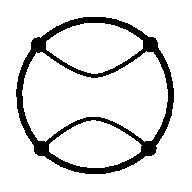
\includegraphics[height=2cm]{capcupresolution.eps}}}\\
\vcenter{\hbox{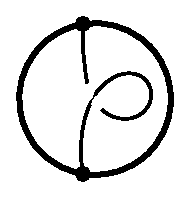
\includegraphics[height=2cm, keepaspectratio]{invvh.eps}}} \quad &= \quad -s^{3}\,\, \vcenter{\hbox{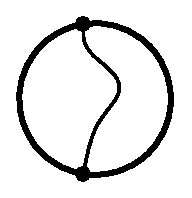
\includegraphics[height=2cm, keepaspectratio]{frameresolution.eps}}}. \notag
\end{align}

Given any 3-manifold, there is a natural map $\sk_s(M) \to K_s(M)$, which follows from the fact that the Kauffman bracket skein relations imply the Kauffman skein relations. If $M = F \times [0,1]$ for some surface $F$, then this is an algebra map.

%\PS{include Kauffman bracket skein relations}

The Frohman and Gelca presentation of the Kauffman bracket skein algebra uses the Chebyshev polynomials $T_n(x)$, which are uniquely characterized by the property $T_n(X+X^{-1}) = X^n + X^{-n}$. If $\xx \in \Z^2$ with $d(\xx) = k$, they defined an element $e_\xx \in K_s(T^2)$ by 
\[
e_\xx := T_k(\alpha_{\xx / k})
\]
where $\alpha_\xx$ is the simple closed curve of slope $\xx$.

\begin{lemma}
	The algebra map $\sk_s(T^2\times [0,1]) \to K_s(T^2\times [0,1])$ takes the generator $D_\xx$ to  $e_\xx$.
\end{lemma}
\begin{proof}
The closure of the symmetrizer $f_n$ in the annulus gets sent to the (closure of the) Jones-Wenzl idempotent in the Kauffman bracket skein algebra of the annulus, because both symmetrizers are uniquely determined by the way they absorb crossings and caps. Under the identification $K_s(S^1\times D^2) = \C[x]$, the closure of the Jones-Wenzl idempotent is sent to $S_n(x)$, the other version of the Chebyshev polynomial, which is defined by 
\[S_n(X+X^{-1}) = \frac{X^{n+1}-X^{-n-1}}{X-X^{-1}}.\]
All that is left to show is that the $S_n(x)$ and $T_n(x)$ satisfy the power series identity in Definition \ref{def:dk}, which we write as
\begin{equation*}
\sum_{k=1}^\infty \frac{T_k(x)}{k} t^k =\ln\left(1 + \sum_{j \geq 1} S_j(x) t^j\right).
\end{equation*}	
% \PS{add proof of this identity (later)} \AP{added a sketch}
Define different variants of  Chebyshev polynomials via $C_n^S(x/2):=S(x)$ and $2C_n^T(x/2):=T(x)$. The following two identities are well known (see, e.g. any book on special functions, or Wikipedia):
\begin{align*}
	\sum_{n \geq 0} C_n^S(x)t^n &= \frac{1}{1-2tx+t^2} \\
	\sum_{n \geq 1} C_n^T(x)\frac{t^n}{n} &= \ln \left( \frac{1}{\sqrt{1-2tx+t^2}} \right).
\end{align*}
The first identity implies 
\[
	1+\sum_{n \geq 1} S_n(x)t^n = \frac{1}{1-tx+t^2}.
\]
This implies the follow identities:
\begin{equation*}
	1+\sum_{n \geq 1} S_n(x)t^n  = \frac{1}{1-tx+t^2} = \left( \exp \left( \sum_{n \geq 1} C_n^T(x/2)\frac{t^n}{n} \right) \right)^2
	= \exp \left( \sum_{n \geq 1} 2 C_n^T(x/2)\frac{t^n}{n} \right).
\end{equation*}
This leads to the following, which completes the proof:
\begin{equation*}
\ln \left( 1+\sum_{n \geq 1} S_n(x)t^n \right) = \sum_{n \geq 1} 2 C_n^T(x/2)\frac{t^n}{n} = \sum_{n \geq 1} \frac{T_n(x)}{n} t^n.
\end{equation*} 
\end{proof}

Now let us recall the description of the Kauffman bracket skein algebra of the torus given by Frohman and Gelca.
\begin{theorem}[{\cite{FG00}}]\label{thm:fg}
	The Kauffman bracket skein algebra $K_s(T^2)$ has a presentation with generators $e_\xx$ and relations
	\begin{align}
	e_\xx e_\yy &= s^d e_{\xx + \yy} + s^{-d} e_{\xx-\yy}\label{eq:fgrel}\\
	e_{\xx} &= e_{-\xx}\notag
	\end{align}
	where $d = \det[\xx\,\yy]$.
\end{theorem}

A short computation using this presentation shows  the commutator identity
\begin{equation}\label{eq:fg}
[e_\xx, e_\yy] = (s^d-s^{-d}) (e_{\xx+\yy} - e_{\xx-\yy}).
\end{equation}
In other words, the relations we show for $D_\xx \in \sk(T^2)$ get sent to the relations in \eqref{eq:fg}, and the relations Frohman and Gelca showed in Theorem \ref{thm:fg} for the $e_\xx \in K_s(T^2)$ imply the relations in \eqref{eq:fg}. This shows our results are compatible with those of Frohman and Gelca.

\begin{remark}\label{rmk:sobig}
We emphasize that the algebra we describe is much bigger -- $\sk(T^2)$ has a linear basis given by unordered words in the $D_\xx$, while the Kauffman bracket skein algebra $K_s(T^2)$ has a linear basis given by the $e_\xx$ themselves. This happens because the Kauffman bracket skein relations allow all crossings to be removed from a diagram, so the algebra is spanned (over $R$) by curves without crossings. However, the more general Kauffman relations only allow crossings to be flipped, and not removed, which means the algebra is spanned (over $R$) by products of knots (which may have self-crossings). In particular, the relations \eqref{eq:fgrel} do not hold in the Kauffman skein algebra $\cd$.
\end{remark}


\chapter{More Formulas and Partial Results}


\section{Commutation Relations For BMW and Hecke Symmetrizer Closures} \label{sec:morecommutationrelations}

This next theorem follows directly from Equation \eqref{eq:skewcommutator2}, which makes it equivalent to Theorem \ref{thm:powersumcommutator} in some sense. This expresses the left $\cd(A)$-action on $\ca_\cd$ in terms of the right action, and vice versa. This implies a commutation relation for the closures of the BMW symmetrizers in terms of either the elements of the set $\{\tilde{h}_j \cdot a^i \}_{j, i}$ or $\{ a^i \cdot \tilde{h}_j \}_{j, i \geq 0}$ which are subsets of the bases $\{ \widetilde{Q}_\lambda \cdot a^i \}_{i \geq 0, \lambda}$ and $\{ a^i \cdot \widetilde{Q}_\lambda \}_{i \geq 0, \lambda}$ of $\ca_\cd$, respectively. These supersets are bases since $\ca_\cd = \cd(A)[a, a^{-1}]$ as algebras in the category of left $\cd(A)$-modules and because the map defined by $\widetilde{Q}_\lambda \cdot a^i \mapsto a^i \cdot \widetilde{Q}_\lambda$ is an invertible algebra homomorphism. 

\begin{theorem} \label{prop:hncommutator}
For any $n \geq 1$, the relations
\begin{equation}
\tilde{h}_n \cdot e = \sum_{i=0}^n d_i (e \cdot \tilde{h}_{n-i})
\end{equation}
and
\begin{equation}
e \cdot \tilde{h}_n = \sum_{i=0}^n \bar{d}_i (\tilde{h}_{n-i} \cdot e)
\end{equation}
hold in $\ca_\cd$, where
\begin{align*}
d_0 & = 1, \\
d_i & = \sum_{l=0}^{i-1} (1 - s^2) s^{2l-i} a^{i-2l} + (1 - s^{-2}) s^{i-2l} a^{2l-i} \qquad \forall i \geq 1, \\
\bar{d}_i & = \sum_{l=0}^{i-1} (1 - s^{-2}) s^{i-2l} a^{i-2l} + (1 - s^{2}) s^{2l-i} a^{2l-i} \qquad \forall i \geq 1.
\end{align*}
Equivalently,
\begin{equation}
e \cdot \tilde{h}_n - \tilde{h}_n \cdot e = \sum_{i=1}^n \bar{d}_i (\tilde{h}_{n-i} \cdot e)
\end{equation}
or 
\begin{equation}
\tilde{h}_n \cdot e - e \cdot \tilde{h}_n = \sum_{i=1}^n d_i (e \cdot \tilde{h}_{n-i}).
\end{equation}
\end{theorem}
\begin{proof}
The formulas for the $d_i$ were discovered experimentally by coding a solver using the SymPy package in Python. The second equation is just the mirror map applied to the first equation, so we will just prove the first equation.

The idea of the proof depends on a reformulation of Equation \eqref{eq:skewcommutator2} as
\[
\tilde{h}_n \cdot e = e \cdot \tilde{h}_n - ( s a + s^{-1} a^{-1} ) ( e \cdot \tilde{h}_{n-1} ) + e \cdot \tilde{h}_{n-2} + ( s^{-1} a + s a^{-1} ) \tilde{h}_{n-1} \cdot e - \tilde{h}_{n-2} \cdot e
\]
and a recursive application of this formula to its last two terms on the right-hand side of the equation. 

The case of $n=0$ is trivial. For $n=1$, just apply the Kauffman skein relation. Now assume the induction hypothesis, that the formula in the statement is true for all $k \leq n-1$. Then apply this assumption to Equation \eqref{eq:skewcommutator2}:
\begin{align*}
\tilde{h}_n \cdot e &= e \cdot \tilde{h}_n - ( s a + s^{-1} a^{-1} ) ( e \cdot \tilde{h}_{n-1} ) + e \cdot \tilde{h}_{n-2} + ( s^{-1} a + s a^{-1} ) ( \tilde{h}_{n-1} \cdot e ) - \tilde{h}_{n-2} \cdot e \\
&= e \cdot \tilde{h}_n - ( s a + s^{-1} a^{-1} ) ( e \cdot \tilde{h}_{n-1} ) + e \cdot \tilde{h}_{n-2} + ( s^{-1} a + s a^{-1} ) \sum_{i=0}^{n-1} d_i (e \cdot \tilde{h}_{n-1-i}) \\
&\quad \,\, - \sum_{i=0}^{n-2} d_i (e \cdot \tilde{h}_{n-2-i}) \\
&= e \cdot \tilde{h}_n + d_1 ( e \cdot \tilde{h}_{n-1} ) + ( s^{-1} a + s a^{-1} ) \sum_{i=1}^{n-1} d_i (e \cdot \tilde{h}_{n-1-i}) - \sum_{i=1}^{n-2} d_i (e \cdot \tilde{h}_{n-2-i}) \\
&= e \cdot \tilde{h}_n + d_1 ( e \cdot \tilde{h}_{n-1} ) + ( s^{-1} a + s a^{-1} ) \sum_{i=0}^{n-2} d_{i+1} (e \cdot \tilde{h}_{n-2-i}) - \sum_{i=1}^{n-2} d_i (e \cdot \tilde{h}_{n-2-i}) \\
&= e \cdot \tilde{h}_n + d_1 ( e \cdot \tilde{h}_{n-1} ) + ( s^{-1} a + s a^{-1} ) d_1 ( e \cdot \tilde{h}_{n-2} ) \\
&\quad\,\, + \sum_{i=1}^{n-2} \big( ( s^{-1} a + s a^{-1} ) d_{i+1} - d_i \big) (e \cdot \tilde{h}_{n-2-i}). \\
\end{align*}
It is a straightforward computation to show that $( s^{-1} a + s a^{-1} ) d_1 = d_2$:
\begin{align*}
( s^{-1} a + s a^{-1} ) d_1 &= ( s^{-1} a + s a^{-1} ) \big( ( 1 - s^2 ) s^{-1} a + ( 1 + s^{-2} ) s a^{-1} \big) \\
&= ( 1 - s^2 ) s^{-2} a^2 + (1 - s^{-2} ) s^0 a^0 + ( 1 - s^2 ) s^0 a^0 + ( 1 - s^{-2} ) s^2 a^{-2} \\
&= d_2.
\end{align*}
It's slightly more tedious to show that $( s^{-1} a + s a^{-1} ) d_{i+1} - d_i = d_{i+2}$ for all $i \geq 1$:
\begin{eqnarray*}
&&( s^{-1} a + s a^{-1} ) d_{i+1} - d_i \\
=&& ( s^{-1} a + s a^{-1} ) \sum_{l=0}^{i} (1 - s^2) s^{2l-i} a^{i-2l} + (1 - s^{-2}) s^{i-2l} a^{2l-i} \\
&-& \sum_{l=0}^{i-1} (1 - s^2) s^{2l-(i-1)} a^{(i-1)-2l} + (1 - s^{-2}) s^{(i-1)-2l} a^{2l-(i-1)} \\
=&& \sum_{l=0}^{i} (1 - s^2) s^{2l-(i+1)} a^{(i+1)-2l} + (1 - s^{-2}) s^{(i+1)-2l} a^{2l-(i+1)} \\
&+& \sum_{l=0}^{i} (1 - s^2) s^{2l-(i-1)} a^{(i-1)-2l} + (1 - s^{-2}) s^{(i-1)-2l} a^{2l-(i-1)} \\
&-& \sum_{l=0}^{i-1} (1 - s^2) s^{2l-(i-1)} a^{(i-1)-2l} + (1 - s^{-2}) s^{(i-1)-2l} a^{2l-(i-1)} \\
=&& \sum_{l=0}^{i} (1 - s^2) s^{2l-(i+1)} a^{(i+1)-2l} + (1 - s^{-2}) s^{(i+1)-2l} a^{2l-(i+1)} \\
&+& (1 - s^2) s^{i+1} a^{-1-i} + (1 - s^{-2}) s^{-1-i} a^{i+1} \\
=&& d_{i+2}.
\end{eqnarray*}
This completes the proof of the statement. 
\end{proof}

\begin{remark}
There exists an algebra homomorphism from $\cd(A)$ to the ring of symmetric functions $\Lambda_R$ (see Section \ref{sec:Lukac}). Conjecturally, this map is an isomorphism, which would imply that the sets $\{ \tilde{h}_\lambda \cdot a^i \}_{\lambda, i}$ and $\{ a^i \cdot \tilde{h}_\lambda \}_{\lambda, i}$ over integers $i$ and partitions $\lambda$, where $\tilde{h}_\lambda := \tilde{h}_{\lambda_1} \cdots \tilde{h}_{\lambda_r}$, form bases of $\ca_\cd = \cd(A)[a, a^{-1}]$. If so, then Theorem \ref{prop:hncommutator} provides transition formulas between these two bases, which would then give a full description of $\ca_\cd$ as a $\cd(A)$-$\cd(A)$-bimodule. 
\end{remark}

One might expect similar formulas to hold in the HOMFLYPT case. To our knowledge, there is no HOMFLYPT analogue of Theorem \ref{prop:hncommutator} written down in the literature. Let's do that here. 

\begin{lemma} \label{lem:homfly1}
For all integers $n$, the following relation holds in $\ca_\ch$
\begin{equation}
e \cdot h_n - h_n \cdot e = s a \cdot h_{n-1} - h_{n-1} \cdot  s^{-1} a
\end{equation}
where we use the convention $h_0 = 1$ and $h_n = 0$ if $n < 0$. 
\end{lemma}
\begin{proof}
Recall the power sum elements $P_k$ satisfy the power series equation
\begin{equation} \label{def:Pk}
\sum_{k=1}^\infty \frac{P_k}{k} x^k = \ln \Big( \sum_{n=0}^\infty h_n x^n \Big)
\end{equation}
By Theorem 4.2 of \cite{Mor02b}, the power sum elements satisfy a commutation relation in $\ca_\ch$
\begin{equation}
e \cdot P_k - P_k \cdot e = (s^{k} - s^{-k}) a^k
\end{equation} 
which may be rephrased as a power series equation 
\[
e \cdot \Big( \sum_{k=1}^\infty \frac{P_k}{k} x^k \Big) - \Big( \sum_{k=1}^\infty \frac{P_k}{k} x^k \Big) \cdot e = \sum_{k=1}^\infty s^k a^k - \sum_{k=1}^\infty s^{-k} a^k.
\]
On the left-hand side, use the defining equation \eqref{def:Pk}. Use the power series formulation of natual log on the right-hand side. So we have
\[
\ln \Bigg( e \cdot \Big( \sum_{k=0}^\infty h_k x^k \Big) \Bigg) - \ln \Bigg( \Big( \sum_{k=0}^\infty h_k x^k \Big) \cdot e \Bigg) = \ln ( 1 - s a x ) - \ln ( 1 - s^{-1} a x ).
\]
After moving terms around, using properties of natural log, and exponentiating both sides, we arrive at the equation
\[
\Big( \sum_{n=0}^\infty (h_n \cdot e ) x^n \Big) ( 1 - s a x ) = \Big( \sum_{n=0}^\infty ( e \cdot h_n ) x^k \Big) ( 1 - s^{-1} a x )
\]
which implies the statement of the lemma.
\end{proof}

Recall that the algebra $\ca_\ch$ is equal to the Laurent polynomial ring $\ch(A)^+[a, a^{-1}]$. Under the isomorphism between $\ch(A)^+$ and the ring of symmetric functions $\Lambda_R$, the $h_n$ identify with the complete homogeneous symmetric functions. It is well-known that ordered monomials in the complete homogeneous symmetric functions form a basis of $\Lambda$, hence the sets $\{h_\lambda \cdot a^i \}_{\lambda, i}$ and $\{a^i \cdot h_\lambda \}_{\lambda, i}$ over integers $i$ and partitions $\lambda$, where $h_\lambda := h_{\lambda_1} \cdots h_{\lambda_r}$, form bases of $\ca_\ch$. The following theorem gives transition formulas between these two bases. 

\begin{theorem} \label{prop:homfly2}
The Hecke symmetrizers $h_n$ satisfy the equations
\[
h_n \cdot e = e \cdot h_n + ( 1 - s^2 ) \sum_{l=1}^{n} s^{-l} ( a^l \cdot h_{n-l} )
\]
and
\[
e \cdot h_n = h_n \cdot e + (1 - s^{-2} ) \sum_{l=1}^{n} s^l ( h_{n-l} \cdot a^l ).
\]
\end{theorem}
\begin{proof}
We will prove the first equality. The second is completely analagous. Proceed by induction. When $n=1$, the statement follows from the HOMFLY skein relation. 

We can rearrange the terms of Lemma \ref{lem:homfly1} to get
\begin{equation} \label{eq:homfly1b}
h_n \cdot e = e \cdot h_n + s^{-1} a ( h_{n-1} \cdot e ) - s a ( e \cdot h_{n-1} ).
\end{equation}
By the induction hypothesis,
\begin{align*}
h_n \cdot e & = e \cdot h_n + s^{-1} a ( h_{n-1} \cdot e ) - s a ( e \cdot h_{n-1} ) \\
& = e \cdot h_n + s^{-1} a \Big( e \cdot h_{n-1} + ( 1 - s^2 ) \sum_{j=1}^{n-1} s^{-j} a^j ( e \cdot h_{n-1-j} ) \Big) - s a ( e \cdot h_{n-1} ) \\
& = e \cdot h_n + ( s^{-1} - s ) a ( e \cdot h_{n-1} ) + ( 1 - s^2 ) \sum_{j=1}^{n-1} s^{-j-1} a^{j+1} ( e \cdot h_{n-1-j} ) \\ 
& = e \cdot h_n + ( 1 - s^2 ) s^{-1} a ( e \cdot h_{n-1} ) + ( 1 - s^2 ) \sum_{j=1}^{n-1} s^{-(j+1)} a^{j+1} ( e \cdot h_{n-(j+1)} ) \\
&= e \cdot h_n + ( 1 - s^2 ) \sum_{l=1}^{n} s^{-l} a^{l} ( e \cdot h_{n-l} )
\end{align*}
where the last equality follows from the substitution $j=l+1$. 
\end{proof}






\section{Type B/C/D Schur Functions and BMW Idempotent Closures} \label{sec:Lukac}
In \cite{Luk05}, it is shown using skein theory techniques that there is an algebra isomorphism between the ring of symmetric functions $\Lambda$ and the positive part of the skein algebra of the annulus $\ch(A)^+$. The isomorphism is defined on generators by sending the complete homogeneous symmetric functions to the annular closures of Hecke symmetrizers. Futhermore, it is shown that the image of the Schur function $s_\lambda$ is the idempotent closure $Q_\lambda$. This fact has many implications. For example, the structure constants of $\ch(A)^+$ in the basis $\{ Q_\lambda \}_\lambda$ are the Littlewood-Richardson constants. Also, the definition of $P_k$ implies that these elements truly correspond with the power sum symmetric functions. Through this isomorphism, one could transfer structure of $\Lambda$ to $\ch(A)^+$, such as the Hopf algebra structure or the plethysm structure (see \cite{MM08}). 

From a Lie-theoretic perspective, the ring of symmetric polynomials $\Lambda_N$ in $N$ variables is the ring of polynomial representations of $GL_n(\C)$. There are maps of graded rings $\Lambda_n \to \Lambda_{n-1}$ defined by specializing the $N^{\mathrm{th}}$ variable to $0$, which together form an inverse system whose inverse limit in the category of graded rings is isomorphic to $\Lambda$. This strengthens the existing relationship between the HOMFLYPT skein theory and $GL_n(\C)$ (recall that the skein relations are modeled after relations of morphisms in $U_q(\mathfrak{gl}_n)$-Mod). 

This section is an attempt to emulate Lukac's argument in the Dubrovnik case. First we will review some of the theory behind character rings of the orthogonal and symplectic groups. In particular, they are isomorphic as rings and there are ``Schur functions" indexed over partitions for the different types. Next, for any of the character rings, we can define a homomorphism to $\cd(A)$. We conjecture that the Schur functions are sent to the annular closures of the BMW idempotents $\widetilde{Q}_\lambda$, and we prove the conjecture when the length of $\lambda$ is at most $2$.








\subsection{Universal Character Rings of Orthogonal and Symplectic Type}

Here we will summarize some results from \cite{KT87}. Recall that a character of a (finite-dimensional) group representation is the post-composition of the representation with the trace function. The character of a direct sum of representations is the pointwise sum of the individual characters. Also, the character of a tensor product of representations is the pointwise product of the individual characters. For compact connected Lie groups $G$, two representations of $G$ are isomorphic only if their characters are equal. In this way, the character ring of $G$ is a decategorification of the category of finite-dimensional representations of $G$. Let $R(B_n)$, $R(C_n)$, and $R(D_n)$ denote the character rings of the Lie groups $SO_{2n+1}(\C)$, $SP_{2n}(\C)$, and $SO_{2n}(\C)$ respectively (the type $D_n$ case will require some subtle care, but we will not address these issues here). 

The irreducible representations of $SO_{2n+1}(\C)$ and $SP_{2n}(\C)$ are indexed by partitions $\lambda$ of length at most $n$, and denote their respective characters by $sb_{n, \lambda}$ and $sc_{n, \lambda}$ respectively. Let $sd_{n, \lambda}$ denote the character of the restriction of the appropriate irreducible representation of $O_{2n}(\C)$ to $SO_{2n}(\C)$. These are called the \textbf{Schur polynomials} of types $B_n$, $C_n$, and $D_n$.

Let $G$ be any of $SO_{2n+1}(\C)$, $SP_{2n}(\C)$, and $SO_{2n}(\C)$. A character of $G$ is determined by its value on a maximal torus of $G$, which may be chosen to be a set of diagonal matrices. 
\begin{align*}
&B_n: &\quad T &= \{ \textrm{diag}(t_1, \dots, t_n, 1, t_n^{-1}, \dots, t_1^{-1}) \} \\ 
&C_n: &\quad T &= \{ \textrm{diag}(t_1, \dots, t_n, t_n^{-1}, \dots, t_1^{-1}) \} \\ 
&D_n: &\quad T &= \{ \textrm{diag}(t_1, \dots, t_n, t_n^{-1}, \dots, t_1^{-1}) \}
\end{align*}
Furthermore, it can be shown that $R(G) = \Z[t_1^{\pm 1}, \dots, t_n^{\pm 1}]^{\Z_2^n \rtimes \mathfrak{S}_n} = \Z[t_1+t_1^{-1}, \dots, t_n+t_n^{-1}]^{\mathfrak{S}_n}$. This is isomorphic to the ring of symmetric polynomials $\Lambda_n = \Z[c_1, \dots, c_n]^{S_n}$ under the identification $c_i = t_i + t_i^{-1}$. 

Let $V$ be the natural representation of the group $G$. Let $h_{G,i} := \textrm{Sym}^i(V)$ and $e_{G,i} := \textrm{Alt}^i(V)$ be the symmetric and alternating powers of $V$. Also, let $h_{G,i}^\circ = h_{G,i} - h_{G_i-2}$ and $e_{G,i}^\circ = e_{G,i} - e_{G_i-2}$. The following statements are true.
\begin{enumerate}
\item The characters $h_{B_n,i}^\circ$ and $e_{B_n,i}$ are irreducible, and \[R(B_n) = \Z[h_{B_n,1}^\circ, \dots, h_{B_n,n}^\circ] = \Z[e_{B_n,1}, \dots, e_{B_n,n}]. \]
\item The characters $h_{C_n,i}$ and $e_{C_n,i}^\circ$ are irreducible, and  \[R(C_n) = \Z[h_{C_n,1}, \dots, h_{C_n,n}] = \Z[e_{C_n,1}^\circ, \dots, e_{C_n,n}^\circ]. \]
\item The characters $h_{D_n,i}^\circ$ are irreducible, $e_{D_n,i}$ is irreducible if $i \neq n$, and \[R(D_n) = \Z[h_{D_n,1}^\circ, \dots, h_{D_n,n}^\circ] = \Z[e_{D_n,1}, \dots, e_{D_n,n}]. \]
\end{enumerate}
The characters $h_{G,i}$ are equal to the Schur polynomials corresponding to a single row, and $e_{G_i}$, a single column.

The ring $\Lambda_n$ is called the ring of symmetric polynomials in $n$ indeterminates, and it may be identified with the character ring of finite-dimensional polynomial representations of the Lie group $GL_n(\C)$. The projection maps $\Lambda_n \to \Lambda_{n-1}$ form an inverse system in the category of graded rings, whose inverse limit is what we call the \textbf{ring of symmetric functions} $\Lambda$. The ring $\Lambda$ may be concretely defined as the restriction of the ring of formal power series in countable many indeterminates to those series which have bounded degree and which are invariant under permutations of the indeterminates. 

There are symmetric functions $sb_\lambda=sd_\lambda$ (they are equal) which project to the Schur polynomials $sb_{n,\lambda}$ and $sd_{n, \lambda}$ under the projections. Similarly, there are $sc_\lambda$ which project to $sc_{n, \lambda}$. These symmetric functions are called \text{Schur functions} of types B, C, and D. The sets $\{sb_\lambda \}_\lambda$ and $\{sc_\lambda \}_\lambda$ form $\Z$-bases of $\Lambda$. Furthermore, there is an involutive algebra automorphism defined by $\omega(sb_\lambda) = sc_{\lambda^t}$ where $\lambda^t$ is the transpose partition of $\lambda$. This implies that the structure constants for both bases totally coincide, i.e. if 
\[
sb_{\mu} sb_{\nu} = \sum_\lambda b_{\mu \nu}^\lambda sb_\lambda
\]
and
\[
sc_{\mu} sc_{\nu} = \sum_\lambda c_{\mu \nu}^{\lambda} sc_{\lambda}
\]
then $c_{\mu \nu}^\lambda = b_{\mu^t \nu^t}^{\lambda^t}$. In particular, if we let $hb_i := sb_{(i)}$ be the Schur functions of type B corresponding to one row and $ec_i := sc_{(1^i)}$ be the Schur functions of type C corresponding to one column, then 
\begin{equation} \label{eq:omega1}
\omega(hb_i) = ec_i.
\end{equation}
Let $hb_i^\circ := hb_i - hb_{i-2}$. For a partition $\lambda=(\lambda_0, \lambda_1, \dots, \lambda_{r-1})$ of length $r$, set $hb_\lambda^\circ(i,j) := hb_{\lambda_i - i + j}^\circ + hb_{\lambda_i - i - j}^\circ$. The classical Jacobi-Trudi formula for the type A case generalizes to the type B case as
\begin{equation} \label{eq:jacobitrudi}
sb_\lambda = \frac{1}{2} \det \big( hb_\lambda(i, j) \big)_{0 \leq i, j \leq r-1}
\end{equation}
which implies a type C generalization by applying Equation \eqref{eq:omega1}. The $1/2$ is there simply to compensate for the first column for when $j=0$. 


\subsection{Determinantal Calculations}

The computations in this section will be very technical. Let's fix some notation to hopefully make everything slightly easier to read. First, let
\begin{align*}
t_n &:= \tilde{h}_n \cdot e - e  \cdot \tilde{h}_n, \\
h(n, k) &:= \tilde{h}_{n+k} + \tilde{h}_{n-k}, \\
t(n, k) &:= t_{n+k} + t_{n-k} = h(n, k) \cdot e - e \cdot h(n, k).
\end{align*}
Let's also define the `skew commutator' elements
\begin{align*}
\varsigma^+ (n, k) &:= s^{-1} h(n, k) \cdot a - s a \cdot h(n, k) \\
\varsigma^- (n, k) &:=  s h(n, k) \cdot a^{-1} - s^{-1} a^{-1} \cdot h(n, k).
\end{align*}
It might be worth pointing out these simple relations: 
\begin{equation}
\begin{split}
t(n, -k) &= t(n, k), \\
h(n, -k) &= h(n, k), \\
\varsigma^\pm (n, -k) &= \varsigma^\pm (n, k), \\
t(n, 0) &= 2 t_n, \\
h(n, 0) &= 2 \tilde{h}_n. \\
\end{split}
\end{equation}
There is a way to write a commutator in terms of skew commutators. This is given by the equation
\begin{equation} \label{eq:skewcommutator3}
t(n, k) = \frac{-1}{s-s^{-1}} \big( a^{-1} \varsigma^+(n, k) - a \varsigma^-(n, k) \big)
\end{equation}
for all $k \geq 0$. Also, we may restate the identity of Lemma \ref{lem:powersumcommutator1} in terms of this new notation.
\begin{equation} \label{eq:skewcommutator2}
t(n, 1) = \frac{1}{2} \varsigma^+ (n, 0) + \frac{1}{2} \varsigma^- (n, 0)
\end{equation}

\begin{lemma} \label{lemma:skewcommutatordecomp}
For all $k \geq 0$, the following holds in $\ca$.
\[
t(n, k+1) =  \varsigma^+ (n, k) + \varsigma^- (n, k) - t(n, k-1)
\]
\end{lemma}
\begin{proof}
The base case is $2$ times Equation \ref{eq:skewcommutator2} since $t(n, 1) = t(n, -1)$. To show the general case, use equation \eqref{eq:skewcommutator2} twice.
\begin{align*}
t(n, k+1)
&= t_{n+(k+1)} + t_{n-(k+1)} \\
&= \big( ( s^{-1} \tilde{h}_{n+k} \cdot e - s e \cdot \tilde{h}_{n+k} ) a + ( s \tilde{h}_{n+k} \cdot e - s^{-1} e \cdot \tilde{h}_{n+k} ) a^{-1} - t_{n+(k-1)} \big) \\
&\qquad + \big( ( s^{-1} \tilde{h}_{n-k} \cdot e - s e \cdot \tilde{h}_{n-k} ) a + ( s \tilde{h}_{n-k} \cdot e - s^{-1} e \cdot \tilde{h}_{n-k} ) a^{-1} - t_{n-(k-1)} \big) \\
&= \big( s^{-1} h(n, k) \cdot e - s e \cdot h(n, k) \big) a + \big( s h(n, k) \cdot e - s^{-1} e \cdot h(n, k) \big) a^{-1} \\
&\qquad - t(n, k-1) \\
&= \varsigma^+ (n, k) + \varsigma^- (n, k) - t(n, k-1)
\end{align*}
\end{proof}

\begin{remark}
An alternate formulation of the first statement of the lemma above is
\begin{equation} \label{eq:skewcommutator4}
t(n, k+1) + t(n, k-1) = \varsigma^+ (n, k) + \varsigma^- (n, k)
\end{equation}
which is a generalization of Equation \eqref{eq:skewcommutator2}. Also, one may apply the identity to itself recursively to get a closed form for the $t(n,k)$ in terms of skew-commutators, but the closed form splits into cases depending on $k$. Thirdly, this lemma yields a kind of recursive formula for the skew commutators, given as
\begin{equation} \label{eq:skewcommutator5}
\varsigma^+ (n, k) + \varsigma^- (n, k) = \frac{-1}{s-s^{-1}} \Big( a^{-1} \big( \varsigma^+(n, k+1) + \varsigma^+(n, k-1) \big) - a \big( \varsigma^-(n, k+1) + \varsigma^-(n, k-1) \big) \Big)
\end{equation}
which follows from Equation \eqref{eq:skewcommutator3}
\end{remark}

\begin{lemma} \label{lemma:detgymnastics3}
The following identities hold in $\ca$. 
\leavevmode 
\begin{enumerate}
\item
\begin{equation*}
\begin{vmatrix}
h(n, k) \cdot e & \varsigma^+ (n, k) \\
h(m, k) \cdot e & \varsigma^+ (m, k)
\end{vmatrix}
= s^2
\begin{vmatrix}
e \cdot h(n, k) & \varsigma^+ (n, k) \\
e \cdot h(m, k) & \varsigma^+ (m, k)
\end{vmatrix}
\end{equation*}
\item
\begin{equation*}
\begin{vmatrix}
h(n, k) \cdot e & \varsigma^- (n, k) \\
h(m, k) \cdot e & \varsigma^- (m, k) 
\end{vmatrix}
= s^{-2}
\begin{vmatrix}
e \cdot h(n, k) & \varsigma^- (n, k) \\
e \cdot h(m, k) & \varsigma^- (m, k) 
\end{vmatrix}
\end{equation*}
\end{enumerate}
\end{lemma}

\begin{proof}
Here is the computation for the first item. The proof of the second runs completely parallel. First, expand the determinants.
\[
\big( h(n, k) \cdot e \big) \varsigma^+ (m, k) - \big( h(m, k) \cdot e \big) \varsigma^+ (n, k) = s^2 \big( e \cdot h(n, k) \big) \varsigma^+ (m, k) - s^2 \big( e \cdot h(m, k) \big) \varsigma^+ (n, k)
\]
Collect terms in the following way.
\[
\big( h(n, k) \cdot e - s^2 e \cdot h(n, k) \big) \varsigma^+ (m, k) = \big( h(m, k) \cdot e - s^2 e \cdot h(m, k) \big) \varsigma^+(n, k)
\]
The right-hand side is equal to the left-hand side with the indices $n$ and $m$ interchanged. So the equation holds if and only if the left hand side is invariant under permuting $n$ and $m$. Let $P(n,m)$ equal the left-hand side. Expand the product in $P(n, m)$ using the definition of $\varsigma^+(m, k)$
\begin{align*}
P(n, m) & = \big( h(n, k) \cdot e - s^2 e \cdot h(n, k) \big) \varsigma^+ (m, k) \\
& = \big( h(n, k) \cdot e - s^2 e \cdot h(n, k) \big) \big( s^{-1} h(n, k) \cdot a - s a \cdot h(n, k) \big) \\
& = \Big( s^{-1} \big( h(n, k) h(m, k) \big) \cdot e + s^3 e \cdot \big( h(n, k) h(m, k) \big) \\
& \qquad  - s h(n, k) \cdot e \cdot h(m, k) - s h(m, k) \cdot e \cdot h(n, k) \Big) a
\end{align*}
Use that $\cc$ is commutative to get that $P(n, m) - P(m, n) = 0$. This completes the proof. 
\end{proof}

\begin{remark}
It may be worth pointing out that the factor of $a$ in $\varsigma^+(n, k)$ and the factor of $a^{-1}$ in $\varsigma^-(n, k)$ don't affect the identities above. In other words, scaling identity (1) by $a^{-1}$ gives
\begin{equation}
\begin{vmatrix}
h(n, k) \cdot e & s^{-1} h(n, k) \cdot e - s e \cdot h(n, k) \\
h(m, k) \cdot e & s^{-1} h(m, k) \cdot e - s e \cdot h(m, k)
\end{vmatrix}
= s^2
\begin{vmatrix}
e \cdot h(n, k) & s^{-1} h(n, k) \cdot e - s e \cdot h(n, k) \\
e \cdot h(m, k) & s^{-1} h(m, k) \cdot e - s e \cdot h(m, k)
\end{vmatrix}
\end{equation}
and scaling identity (2) by $a$ gives
\begin{equation}
\begin{vmatrix}
h(n, k) \cdot e &  s h(n, k) \cdot e - s^{-1} e \cdot h(n, k) \\
h(m, k) \cdot e & s h(m, k) \cdot e - s^{-1} e \cdot h(m, k)
\end{vmatrix}
= s^{-2}
\begin{vmatrix}
e \cdot h(n, k) & s h(n, k) \cdot e - s^{-1} e \cdot h(n, k) \\
e \cdot h(m, k) & s h(m, k) \cdot e - s^{-1} e \cdot h(m, k)
\end{vmatrix}.
\end{equation}
\end{remark}

The previous two lemmas together imply the next lemma. 

\begin{lemma} \label{lemma:detgymnastics4}
For all $k \geq 0$, we have
\begin{align*}
&\quad \,
\begin{vmatrix}
h(n, k) \cdot e & t(n, k+1) \\
h(m, k) \cdot e & t(m, k+1)
\end{vmatrix} \\
&=
\begin{vmatrix}
e \cdot h(n, k) & s^2 \varsigma^+ (n, k) + s^{-2} \varsigma^- (n, k) - t(n, k-1) \\
e \cdot h(m, k) & s^2 \varsigma^+ (m, k) + s^{-2} \varsigma^- (m, k) - t(m, k-1)
\end{vmatrix}\\
& \qquad +
\sum_{l=1}^{k}
\begin{vmatrix}
e \cdot h(n, k-l) & (s^2 - 1) \varsigma^+ (n, k-l) + (s^{-2} - 1) \varsigma^- (n, k-l) \\
e \cdot h(m, k-l) & (s^2 - 1) \varsigma^+ (m, k-l) + (s^{-2} - 1) \varsigma^- (m, k-l)
\end{vmatrix}.
\end{align*} 
\end{lemma}
\begin{proof}
First, when $k=0$, the statement should be read as
\begin{align*}
\begin{vmatrix}
h(n, 0) \cdot e & t(n, 1) \\
h(m, 0) \cdot e & t(m, 1)
\end{vmatrix} 
=
\frac{1}{2}
\begin{vmatrix}
e \cdot h(n, k) & s^2 \varsigma^+ (n, 0) + s^{-2} \varsigma^- (n, 0)\\
e \cdot h(m, k) & s^2 \varsigma^+ (m, 0) + s^{-2} \varsigma^- (m, 0)
\end{vmatrix}
\end{align*}
which follows straightforwardly by applying Equation \ref{eq:skewcommutator2} to the entries $t(n,1)$ and $t(m,1)$ before applying Lemma \ref{lemma:detgymnastics3}. In general, use Lemma \ref{lemma:skewcommutatordecomp} to write 
\begin{align*}
\begin{vmatrix}
h(n, k) \cdot e & t(n, k+1) \\
h(m, k) \cdot e & t(m, k+1) \\
\end{vmatrix}
&=
\begin{vmatrix}
h(n, k) \cdot e & \varsigma^+ (n, k) \\
h(m, k) \cdot e & \varsigma^+ (m, k)
\end{vmatrix}
+
\begin{vmatrix}
h(n, k) \cdot e & \varsigma^- (n, k) \\
h(m, k) \cdot e & \varsigma^- (m, k) 
\end{vmatrix} \\
& \quad +
\begin{vmatrix}
h(n, k) \cdot e & - t(n, k-1)\\
h(m, k) \cdot e & - t(m, k-1)
\end{vmatrix}.
\end{align*}
On the first two summands, apply Lemma \ref{lemma:detgymnastics3} to switch the order of the action in the first columns at the price of the specified scalar. For the third summand, observe
\begin{align*}
\begin{vmatrix}
h(n, k) \cdot e & - t(n, k-1) \\
h(m, k) \cdot e & - t(m, k-1) 
\end{vmatrix}
&=
\begin{vmatrix}
t(n, k-1) & h(n, k) \cdot e \\
t(m, k-1) & h(m, k) \cdot e
\end{vmatrix} \\
&= 
\begin{vmatrix}
t(n, k-1) & t(n, k) \\
t(m, k-1) & t(m, k)
\end{vmatrix} 
+
\begin{vmatrix}
t(n, k-1) & e \cdot h(n, k) \\
t(m, k-1) & e \cdot h(m, k)
\end{vmatrix} \\
&=
\begin{vmatrix}
h(n, k-1) \cdot e & t(n, k) \\
h(m, k-1) \cdot e & t(m, k)
\end{vmatrix} 
- 
\begin{vmatrix}
e \cdot h(n, k-1) & t(n, k) \\
e \cdot h(m, k-1) & t(m, k)
\end{vmatrix} \\
& \quad +
\begin{vmatrix}
e \cdot h(n, k) & - t(n, k-1) \\
e \cdot h(m, k) & - t(m, k-1)
\end{vmatrix}.
\end{align*}
Thus, for all $k \geq 0$, we have
\begin{equation}\label{eq:detgymnastics5}
\begin{split}
\begin{vmatrix}
h(n, k) \cdot e & t(n, k+1) \\
h(m, k) \cdot e & t(m, k+1)
\end{vmatrix}
&=
\begin{vmatrix}
e \cdot h(n, k) & s^2 \varsigma^+ (n, k) + s^{-2} \varsigma^- (n, k) - t(n, k-1) \\
e \cdot h(m, k) & s^2 \varsigma^+ (m, k) + s^{-2} \varsigma^- (m, k) - t(m, k-1)
\end{vmatrix} \\
& \quad -
\begin{vmatrix}
e \cdot h(n, k-1) & t(n, k) \\
e \cdot h(m, k-1) & t(m, k)
\end{vmatrix} 
+
\begin{vmatrix}
h(n, k-1) \cdot e & t(n, k) \\
h(m, k-1) \cdot e & t(m, k)
\end{vmatrix}.
\end{split}
\end{equation}
Next, recursively apply Equation \ref{eq:detgymnastics5} to its own trailing term $k$ times so that the right-hand side becomes
\begin{align*}
&\sum_{l=0}^{k-1} \left(
\begin{vmatrix}
e \cdot h(n, k-l) & s^2 \varsigma^+ (n, k-l) + s^{-2} \varsigma^- (n, k-l) - t(n, k-1-l) \\
e \cdot h(m, k-l) & s^2 \varsigma^+ (m, k-l) + s^{-2} \varsigma^- (m, k-l) - t(m, k-1-l)
\end{vmatrix} \right. \\
& \left. \qquad -
\begin{vmatrix}
e \cdot h(n, k-1-l) & t(n, k-l) \\
e \cdot h(m, k-1-l) & t(m, k-l)
\end{vmatrix} \right)
+
\begin{vmatrix}
h(n, 0) \cdot e & t(n, 1) \\
h(m, 0) \cdot e & t(m, 1)
\end{vmatrix}.
\end{align*}
Through some careful reindexing work, we rewrite this as
\begin{align*}
&\begin{vmatrix}
e \cdot h(n, k) & s^2 \varsigma^+ (n, k) + s^{-2} \varsigma^- (n, k) - t(n, k-1) \\
e \cdot h(m, k) & s^2 \varsigma^+ (m, k) + s^{-2} \varsigma^- (m, k) - t(m, k-1)
\end{vmatrix}\\
&+
\sum_{l=1}^{k-1}
\begin{vmatrix}
e \cdot h(n, k-l) & s^2 \varsigma^+ (n, k-l) + s^{-2} \varsigma^- (n, k-l) - t(n, k-1-l) - t(n, k+1-l)\\
e \cdot h(m, k-l) & s^2 \varsigma^+ (m, k-l) + s^{-2} \varsigma^- (m, k-l) - t(m, k-1-l) - t(m, k+1-l)
\end{vmatrix} \\
&-
\begin{vmatrix}
e \cdot h(n, 0) & t(n, 1) \\
e \cdot h(m, 0) & t(m, 1) \\
\end{vmatrix}
+
\begin{vmatrix}
h(n, 0) \cdot e & t(n, 1) \\
h(m, 0) \cdot e & t(m, 1)
\end{vmatrix}.
\end{align*}
Apply Lemma \ref{lemma:skewcommutatordecomp} to the terms in the entries in the second column of each matrix in the big sum. Finally, observe the following applications of Lemmas \ref{lemma:detgymnastics3} and  \ref{lemma:skewcommutatordecomp}:
\begin{align*}
&-
\begin{vmatrix}
e \cdot h(n, 0) & t(n, 1) \\
e \cdot h(m, 0) & t(m, 1) \\
\end{vmatrix}
+
\begin{vmatrix}
h(n, 0) \cdot e & t(n, 1) \\
h(m, 0) \cdot e & t(m, 1)
\end{vmatrix} \\
=& 
-
\begin{vmatrix}
e \cdot h(n, 0) & t(n, 1) \\
e \cdot h(m, 0) & t(m, 1) \\
\end{vmatrix}
+
\begin{vmatrix}
e \cdot h(n, 0) & s^2 \varsigma^+ (n, 0) + s^{-2} \varsigma^- (n, 0) - t(n, -1) \\
e \cdot h(m, 0) & s^2 \varsigma^+ (m, 0) + s^{-2} \varsigma^- (m, 0) - t(m, -1)
\end{vmatrix} \\
=& 
\begin{vmatrix}
e \cdot h(n, 0) & s^2 \varsigma^+ (n, 0) + s^{-2} \varsigma^- (n, 0) - 2 t(n, 1) \\
e \cdot h(m, 0) & s^2 \varsigma^+ (m, 0) + s^{-2} \varsigma^- (m, 0) - 2 t(m, 1)
\end{vmatrix} \\
=& 
\begin{vmatrix}
e \cdot h(n, 0) & (s^2 - 1) \varsigma^+ (n, 0) + (s^{-2} - 1) \varsigma^- (n, 0) \\
e \cdot h(m, 0) & (s^2 - 1) \varsigma^+ (m, 0) + (s^{-2} - 1) \varsigma^- (m, 0)
\end{vmatrix} 
\end{align*}
where we use $t(n, 1) = t(n, -1)$. This completes the proof. 
\end{proof}

\begin{remark} \label{rmk:detgymnastics6}
Using a parallel technique as in the proof of Lemma \ref{lemma:detgymnastics4}, one can show that
\begin{align*}
& \quad \,
\begin{vmatrix}
e \cdot h(n, k) & t(n, k+1) \\
e \cdot h(m, k) & t(m, k+1)
\end{vmatrix} \\
&=
\begin{vmatrix}
h(n, k) \cdot e & s^{-2} \varsigma^+ (n, k) + s^{2} \varsigma^- (n, k) - t(n, k-1) \\
h(m, k) \cdot e & s^{-2} \varsigma^+ (m, k) + s^{2} \varsigma^- (m, k) - t(m, k-1)
\end{vmatrix}\\
& \quad +
\sum_{l=1}^{k}
\begin{vmatrix}
h(n, k-l) \cdot e & (s^{-2} - 1) \varsigma^+ (n, k-l) + (s^{2} - 1) \varsigma^- (n, k-l) \\
h(m, k-l) \cdot e & (s^{-2} - 1) \varsigma^+ (m, k-l) + (s^{2} - 1) \varsigma^- (m, k-l)
\end{vmatrix}.
\end{align*}
\end{remark}

\begin{corollary}
\begin{align*}
\begin{vmatrix}
t(n, k) & t(n, k+1) \\
t(m, k) & t(m, k+1)
\end{vmatrix}
& =
\sum_{l=0}^{k}
\begin{vmatrix}
e \cdot h(n, k-l) & (s^2 - 1) \varsigma^+ (n, k-l) + (s^{-2} - 1) \varsigma^- (n, k-l) \\
e \cdot h(m, k-l) & (s^2 - 1) \varsigma^+ (m, k-l) + (s^{-2} - 1) \varsigma^- (m, k-l)
\end{vmatrix} \\
& = \sum_{l=0}^{k}
\begin{vmatrix}
h(n, k-l) \cdot e & (1 - s^{-2}) \varsigma^+ (n, k-l) + (1 - s^{2}) \varsigma^- (n, k-l) \\
h(m, k-l) \cdot e & (1 - s^{-2}) \varsigma^+ (m, k-l) + (1 - s^{2}) \varsigma^- (m, k-l)
\end{vmatrix}.
\end{align*}
\end{corollary}
\begin{proof}
We prove the first equality. The second follows by using Remark \ref{rmk:detgymnastics6}.
\begin{align*}
&\quad \begin{vmatrix}
t(n, k) & t(n, k+1) \\
t(m, k) & t(m, k+1)
\end{vmatrix} \\
&= - 
\begin{vmatrix}
e \cdot h(n, k) & t(n, k+1) \\
e \cdot h(m, k) & t(m, k+1)
\end{vmatrix} 
+
\begin{vmatrix}
h(n, k) \cdot e & t(n, k+1) \\
h(m, k) \cdot e & t(m, k+1)
\end{vmatrix}
\\
&= - 
\begin{vmatrix}
e \cdot h(n, k) & \varsigma^+ (n, k) + \varsigma^- (n, k) - t(n, k-1) \\
e \cdot h(m, k) & \varsigma^+ (m, k) + \varsigma^- (m, k) - t(m, k-1)
\end{vmatrix} \\
&\quad +
\begin{vmatrix}
e \cdot h(n, k) & s^2 \varsigma^+ (n, k) + s^{-2} \varsigma^- (n, k) - t(n, k-1) \\
e \cdot h(m, k) & s^2 \varsigma^+ (m, k) + s^{-2} \varsigma^- (m, k) - t(m, k-1)
\end{vmatrix}\\
&\quad +
\sum_{l=1}^{k}
\begin{vmatrix}
e \cdot h(n, k-l) & (s^2 - 1) \varsigma^+ (n, k-l) + (s^{-2} - 1) \varsigma^- (n, k-l) \\
e \cdot h(m, k-l) & (s^2 - 1) \varsigma^+ (m, k-l) + (s^{-2} - 1) \varsigma^- (m, k-l)
\end{vmatrix} \\
= & \sum_{l=0}^{k}
\begin{vmatrix}
e \cdot h(n, k-l) & (s^2 - 1) \varsigma^+ (n, k-l) + (s^{-2} - 1) \varsigma^- (n, k-l) \\
e \cdot h(m, k-l) & (s^2 - 1) \varsigma^+ (m, k-l) + (s^{-2} - 1) \varsigma^- (m, k-l)
\end{vmatrix} 
\end{align*}
\end{proof}

Let $\textrm{cl}_\ca : \ca \to \cc$ be the wiring which connects the two boundary points of $\ca$ by an arc above the annulus. 
\begin{figure}[H]
\centering
$\pic[7]{cla.eps}$
\caption{The wiring diagram which defines $\textrm{cl}_\ca : \ca \to \cc$.}
\end{figure}

This map is not unital nor multiplicative, but it is a right $\cc$-module homomorphism so that $\cl_\ca(e \cdot x) = \delta_\cd x$. Furthermore, the closure $\cl_\ca(x \cdot e)$ is the element $\phi(x)$ which is the meridian map $\phi$ applied to $x$. The following identity is a generalization of Lemma 8.3 in Lukac.

\begin{lemma} \label{lemma:tclosure}
Let 
\[
\alpha_n := \{ n \} \left( v^{-1} s^{n - 1} - v s^{1 - n} \right).
\] 
Then, 
\[
\textrm{cl}_\ca \left( \frac{1}{2} t(n,0) \right) = \textrm{cl}_\ca (t_n) = \alpha_n \tilde{h}_n
\]
and hence 
\[
\textrm{cl}_\ca \big( t(n, k) \big) = \alpha_{n+k} \tilde{h}_{n+k} + \alpha_{n-k} \tilde{h}_{n-k}.
\]
\end{lemma}
\begin{proof}
Recall Equation \eqref{eq:annfund}, which we restate here using different notation:
\[
t_n = \{ n \} a^{-1}W^*_{n - 1} - \{ n \} aW_{n - 1}.
\]
Apply the closure to both sides. Apply the framing relation to the diagrams on the right to pick up the framing parameter terms. Use the property that the BMW idempotents absorb crossings to a factor of $s$ for positive crossings and $s^{-1}$ for negative crossings. This completes the proof. 
\end{proof}

\begin{lemma} \label{lemma:skewclosures}
Define the constants
\begin{align*}
\omega_{n}^+ &:= - \{n\} s^{1-n} v, \\
\upsilon_{n}^+ &:= s^{n} [n+1] (\bar{\beta}_{n+1} - \beta_{n+1} ) \big( \delta_\cd + s^{n-1} [n] ( s v^{-1} + \beta_{n} ) \big), \\
\omega_{n}^- &:= \{n\} s^{n-1} v^{-1}, \\
\upsilon_{n}^- &:= -s^{-n} [n+1] ( \bar{\beta}_{n+1} - \beta_{n+1} ) \big( \delta_\cd + s^{n-1} [n] ( s v^{-1} + \beta_{n} ) \big).
\end{align*}
Then the following identities hold in $\cc$ for all $n \geq 0$ 
\begin{align*}
\textrm{cl}_\ca \left( \frac{1}{2} \varsigma^+(n,0) \right) &= \quad \textrm{cl}_\ca \big( s^{-1} \tilde{h}_n \cdot a - s a \cdot \tilde{h}_n \big) \quad = \omega_{n+1}^+ \tilde{h}_{n+1} + \upsilon_{n-1}^+ \tilde{h}_{n-1}, \\
\textrm{cl}_\ca \left( \frac{1}{2} \varsigma^-(n,0) \right) &=\textrm{cl}_\ca \big( s \tilde{h}_n \cdot a^{-1} - s^{-1} a^{-1} \cdot \tilde{h}_n \big) = \omega_{n+1}^- \tilde{h}_{n+1} + \upsilon_{n-1}^- \tilde{h}_{n-1}
\end{align*}
which implies that
\begin{align*}
\textrm{cl}_\ca \big( \varsigma^+ (n, k) \big) &= \omega_{n+k+1}^+ \tilde{h}_{n+k+1} + \upsilon_{n+k-1}^+ \tilde{h}_{n+k-1} + \omega_{n-k+1}^+ \tilde{h}_{n-k+1} + \upsilon_{n-k-1}^+ \tilde{h}_{n-k-1}, \\
\textrm{cl}_\ca \big( \varsigma^- (n, k) \big) &= \omega_{n+k+1}^- \tilde{h}_{n+k+1} + \upsilon_{n+k-1}^- \tilde{h}_{n+k-1} + \omega_{n-k+1}^- \tilde{h}_{n-k+1} + \upsilon_{n-k-1}^- \tilde{h}_{n-k-1}.
\end{align*}
\end{lemma}
\begin{proof}
Apply Equations \eqref{eq:r3} and \eqref{eq:r1} :
\begin{align*}
& \quad \, ( s^{-1} \tilde{h}_n \cdot e - s e \cdot \tilde{h}_n ) a \\
&=  \Big( s^{-1} \big( [n+1] W_n - [n] s a W_{n-1} - [n] s \bar{\beta}_n a^{-1} W^*_{n-1} \big) \\
&\quad \, - s \big( [n+1] W_n - [n] s^{-1} a W_{n-1} - [n] s^{-1} \beta_n a^{-1} W^*_{n-1} \big) \Big) a \\
&= - \{n+1\} a W_n - ( \bar{\beta}_n - \beta_n ) [n] W^*_{n-1}.
\end{align*}
%\AP{There is an endomorphism on the BMW algebra which reflects the square along a vertical line through the middle of the square. Are the symmetrizers fixed by this map? I think you can use the uniqueness of the symmetrizers to prove this since they are idempotent and absorb scalars.} \PS{I agree, they should be fixed}
The identities below hold in $\cc$. Use Lemma 21 from \cite{She16} to prove the second two.
\begin{align*}
\textrm{cl}_\ca ( a W_n ) &= s^{-n} v \tilde{h}_{n+1} \\
\textrm{cl}_\ca ( a^{-1} W^*_n ) &= s^n v^{-1} \tilde{h}_{n+1} \\
\textrm{cl}_\ca ( W_n ) &= -s^{-n} \big( \delta_\cd + s^{n-1} [n] ( s v^{-1} + \beta_n ) \big) \tilde{h}_n \\
&= [n+1]^{-1} \big( \delta_\cd + [n]s^{-1} ( s^{-(n-1)} v - \beta_n s^{n-1} v^{-1} ) \big) \tilde{h}_n \\
\textrm{cl}_\ca ( W^*_n ) &= s^n \big( \delta_\cd + s^{n-1} [n] ( s v^{-1} + \beta_n ) \big) \tilde{h}_n
\end{align*}
Then applying $\textrm{cl}_\ca$ to the above gives
\begin{align*} 
& \textrm{cl}_\ca \big( s^{-1} \tilde{h}_n \cdot a - s a \cdot \tilde{h}_n \big) \\
=& - \{n+1\} \textrm{cl}_\ca ( a W_n ) - ( \bar{\beta}_n - \beta_n ) [n] \textrm{cl}_\ca ( W^*_{n-1} ) \\
= & - \{n+1\} s^{-n} v \tilde{h}_{n+1} - ( \bar{\beta}_n - \beta_n ) [n] s^{n-1} \big( \delta_\cd + s^{n-2} [n-1] ( s v^{-1} \beta_{n-1} ) \big) \tilde{h}_{n-1} \\
= & \omega_{n+1}^+ \tilde{h}_{n+1} + \upsilon_{n-1}^+ \tilde{h}_{n-1}.
\end{align*}
The proof of the other statement is similar. 
\end{proof}

\begin{remark}
As a quick corollary of this lemma, apply $\textrm{cl}_\ca$ to Equation \eqref{eq:skewcommutator4} with $k=0$, so
\[
\textrm{cl}_\ca \big( 2 t(n, 1) \big) = \textrm{cl}_\ca \big( \varsigma^+ (n, 0) + \varsigma^- (n, 0) \big)
\]
and apply the previous two Lemmas and divide by $2$ to get
\[
\alpha_{n+1} \tilde{h}_{n+1} + \alpha_{n-1} \tilde{h}_{n-1} = (\omega^+_{n+1} + \omega^-_{n+1}) \tilde{h}_{n+1} + (\upsilon^+_{n-1} + \upsilon^-_{n-1}) \tilde{h}_{n-1}.
\]
Since the $\tilde{h}_n$ are linearly independent, it's true that 
\begin{equation}
\alpha_n = \omega_n^+ + \omega_n^- = \upsilon_n^+ + \upsilon_n^-
\end{equation}
for any $n$. 
\end{remark}

Consider the algebra homomorphism $\Lambda \to \cd(A)$ defined by the assignment $hb_i \mapsto \tilde{h}_i$. This map is well defined since $\Lambda$ is generated freely as a commutative ring by the set $\{hb_i\}_{i}$. Let $S_\lambda$ be the image of $sb_\lambda$ under this assignment. Now we are ready to state the main conjecture of this section.
\begin{conjecture} \label{conj:schureigenvalues}
Let $\phi: \cc \to \cc$ be the meridian map.  Then
\begin{equation}
\phi ( S_\lambda ) = c_\lambda S_\lambda
\end{equation}
where
\begin{equation}
c_\lambda = \delta_\cd + ( s - s^{-1} ) \Big( v^{-1} \sum_{x \in \lambda} s^{2 \textrm{cn}(x)} - v \sum_{x \in \lambda} s^{-2 \textrm{cn}(x)} \Big)
\end{equation}
and where $\textrm{cn}(x)$ is the content of the cell $x$ of the Young diagram of $\lambda$ in the $(i,j)^{\textrm{th}}$ position, defined by $\textrm{cn}(x) := j-i$.
\end{conjecture}

\AP{make this a corollary}
If true, then this conjecture may be used to prove that $S_\lambda = \widetilde{Q}_\lambda$, following the same arguement from \cite{Luk05}. Essentially, Conjecture \ref{conj:schureigenvalues} states that $S_\lambda$ and $Q_\lambda$ are in the same eigenspace with respect to $\phi$. These eigenspaces each have dimension $1$ by \cite{LZ02}, so $S_\lambda$ would be a scalar multiple of $Q_\lambda$. Following Lukac, a simple induction argument involving the branching formula of \cite{BB01} shows that this scalar is $1$. Next, let's give some evidence for why this conjecture should be true. 

\begin{proposition}
The conjecture holds when $\lambda$ has length at most $2$.
\end{proposition}
\begin{proof}
The statement is trivial if $\lambda$ has length $1$ by definition of the map. Assume $\lambda = (a, b)$. Apply Equation \eqref{eq:jacobitrudi}.
\[
S_\lambda = 
\begin{vmatrix}
\frac{1}{2}\tilde{h}_\lambda(0,0) & \tilde{h}_\lambda(0,1) \\
\frac{1}{2}\tilde{h}_\lambda(1,0) & \tilde{h}_\lambda(1,1)
\end{vmatrix}
\]
Use multilinearity of the determinant as we did above to decompose the commutator $S_\lambda \cdot e - e \cdot S_\lambda$.
\begin{equation*}
S_\lambda \cdot e - e \cdot S_\lambda = 
\begin{vmatrix}
\frac{1}{2} t_\lambda(0,0) & e \cdot \tilde{h}_\lambda(0,1) \\
\frac{1}{2} t_\lambda(1,0) & e \cdot \tilde{h}_\lambda(1,1)
\end{vmatrix}
+
\begin{vmatrix}
\frac{1}{2}\tilde{h}_\lambda(0,0) \cdot e & t_\lambda(0,1) \\
\frac{1}{2}\tilde{h}_\lambda(1,0) \cdot e & t_\lambda(1,1)
\end{vmatrix} \\
\end{equation*}
The entries in the second column of the second determinant need to be split using Equation \eqref{eq:skewcommutator2} into a form which is compatible with Lemma \ref{lemma:detgymnastics3}. The right-hand side becomes
\[
\begin{vmatrix}
\frac{1}{2} t_\lambda(0,0) & e \cdot \tilde{h}_\lambda(0,1) \\
\frac{1}{2} t_\lambda(1,0) & e \cdot \tilde{h}_\lambda(1,1)
\end{vmatrix}
+
\begin{vmatrix}
\frac{1}{2}\tilde{h}_\lambda(0,0) \cdot e & \frac{1}{2} \varsigma_\lambda^+(0,0) \\
\frac{1}{2}\tilde{h}_\lambda(1,0) \cdot e & \frac{1}{2} \varsigma_\lambda^+(1,0)
\end{vmatrix}
+
\begin{vmatrix}
\frac{1}{2}\tilde{h}_\lambda(0,0) \cdot e & \frac{1}{2} \varsigma_\lambda^-(0,0) \\
\frac{1}{2}\tilde{h}_\lambda(1,0) \cdot e & \frac{1}{2} \varsigma_\lambda^-(1,0)
\end{vmatrix}.
\]
Apply Lemma \ref{lemma:detgymnastics3} to the second two terms:
\[
\begin{vmatrix}
\frac{1}{2} t_\lambda(0,0) & e \cdot \tilde{h}_\lambda(0,1) \\
\frac{1}{2} t_\lambda(1,0) & e \cdot \tilde{h}_\lambda(1,1)
\end{vmatrix}
+ s^2
\begin{vmatrix}
e \cdot \frac{1}{2}\tilde{h}_\lambda(0,0) & \frac{1}{2} \varsigma_\lambda^+(0,0) \\
e \cdot \frac{1}{2}\tilde{h}_\lambda(1,0) & \frac{1}{2} \varsigma_\lambda^+(1,0)
\end{vmatrix}
+ s^{-2}
\begin{vmatrix}
e \cdot \frac{1}{2}\tilde{h}_\lambda(0,0) & \frac{1}{2} \varsigma_\lambda^-(0,0) \\
e \cdot \frac{1}{2}\tilde{h}_\lambda(1,0) & \frac{1}{2} \varsigma_\lambda^-(1,0)
\end{vmatrix}.
\]
Now apply $\cl_\ca$ and use the property that it is a right $\cc$-module homomorphism to remove $e$ from the $\tilde{h}_i$ terms. Apply Lemmas \ref{lemma:tclosure} and \ref{lemma:skewclosures} for the second equality.
\begin{align*}
&\quad \textrm{cl}_\ca ( S_\lambda \cdot e - e \cdot S_\lambda ) \\
&=
\begin{vmatrix}
\cl_\ca \big( \frac{1}{2} t_\lambda(0,0) \big) & \tilde{h}_\lambda(0,1) \\
\cl_\ca \big( \frac{1}{2} t_\lambda(1,0) \big) & \tilde{h}_\lambda(1,1)
\end{vmatrix}
+ s^2
\begin{vmatrix}
\frac{1}{2}\tilde{h}_\lambda(0,0) & \cl_\ca \big( \frac{1}{2} \varsigma_\lambda^+(0,0) \big) \\
\frac{1}{2}\tilde{h}_\lambda(1,0) & \cl_\ca \big( \frac{1}{2} \varsigma_\lambda^+(1,0) \big)
\end{vmatrix} \\
& \quad + s^{-2}
\begin{vmatrix}
\frac{1}{2}\tilde{h}_\lambda(0,0) & \cl_\ca \big( \frac{1}{2} \varsigma_\lambda^-(0,0) \big) \\
\frac{1}{2}\tilde{h}_\lambda(1,0) & \cl_\ca \big( \frac{1}{2} \varsigma_\lambda^-(1,0) \big)
\end{vmatrix} \\
&=
\begin{vmatrix}
\cl_\ca \big( \frac{1}{2} t(a,0) \big) & \tilde{h}(a,1) \\
\cl_\ca \big( \frac{1}{2} t(b-1,0) \big) & \tilde{h}(b-1,1)
\end{vmatrix}
+ s^2
\begin{vmatrix}
\frac{1}{2}\tilde{h}(a,0) & \cl_\ca \big( \frac{1}{2} \varsigma^+(a,0) \big) \\
\frac{1}{2}\tilde{h}(b-1,0) & \cl_\ca \big( \frac{1}{2} \varsigma^+(b-1,0) \big)
\end{vmatrix} \\
& \quad + s^{-2}
\begin{vmatrix}
\frac{1}{2}\tilde{h}(a,0) & \cl_\ca \big( \frac{1}{2} \varsigma^-(a,0) \big) \\
\frac{1}{2}\tilde{h}(b-1,0) & \cl_\ca \big( \frac{1}{2} \varsigma^-(b-1,0) \big)
\end{vmatrix} \\
&=
\begin{vmatrix}
\alpha_a \tilde{h}_a & \tilde{h}_{a+1} + \tilde{h}_{a-1} \\
\alpha_{b-1} \tilde{h}_{b-1} & \tilde{h}_{b} + \tilde{h}_{b-2}
\end{vmatrix}
+ s^2
\begin{vmatrix}
\tilde{h}_a & \omega_{a+1}^+ \tilde{h}_{a+1} + \upsilon^+_{a-1} \tilde{h}_{a-1} \\
\tilde{h}_{b-1} & \omega_{b}^+ \tilde{h}_{b} + \upsilon^+_{b-2} \tilde{h}_{b-2}
\end{vmatrix} \\
& \quad + s^{-2}
\begin{vmatrix}
\tilde{h}_a & \omega_{a+1}^- \tilde{h}_{a+1} + \upsilon^-_{a-1} \tilde{h}_{a-1} \\
\tilde{h}_{b-1} & \omega_{b}^- \tilde{h}_{b} + \upsilon^-_{b-2} \tilde{h}_{b-2}
\end{vmatrix} \\
&= \big( \alpha_a \tilde{h}_a (\tilde{h}_{b} + \tilde{h}_{b-2}) - \alpha_{b-1} \tilde{h}_{b-1} (\tilde{h}_{a+1} + \tilde{h}_{a-1}) \big) \\
& \quad + s^2 \big( \tilde{h}_a (\omega_{b}^+ \tilde{h}_{b} + \upsilon^+_{b-2} \tilde{h}_{b-2}) - \tilde{h}_{b-1}( \omega_{a+1}^+\tilde{h}_{a+1} + \upsilon^+_{a-1} \tilde{h}_{a-1}) \big) \\
& \quad + s^{-2} \big( \tilde{h}_a (\omega_{b}^- \tilde{h}_{b} + \upsilon^-_{b-2} \tilde{h}_{b-2}) - \tilde{h}_{b-1} (\omega_{a+1}^- \tilde{h}_{a+1} + \upsilon^-_{a-1} \tilde{h}_{a-1}) \big) \\
&= (\alpha_a + s^2 \omega_b^+ + s^{-2} \omega_b^-) \tilde{h}_a \tilde{h}_b + (\alpha_a + s^2 \upsilon_{b-2}^+ + s^{-2} \upsilon_{b-2}^-) \tilde{h}_a \tilde{h}_{b-2} \\
&\quad - (\alpha_{b-1} + s^{2} \omega_{a+1}^+ + s^{-2} \omega_{a+1}^-) \tilde{h}_{a+1} \tilde{h}_{b-1} - (\alpha_{b-1} + s^2 \upsilon_{a-1}^+ + s^{-2} \upsilon_{a-1}^-) \tilde{h}_{a-1} \tilde{h}_{b-1} 
\end{align*}
The conjecture claims that all of these coefficients are equal to the appropriate eigenvalue minus the value of the unknot $c_\lambda - \delta_\cd$. At first glance, it's not at all obvious that these coefficients are even equal to each other. Nevertheless, we will show it is true by looking at each coefficient one by one, going in the order in which they are written. Firstly, observe:
\begin{align*}
\alpha_a + s^2 \omega_b^+ + s^{-2}\omega_b^- &= \{a\} (v^{-1}s^{a-1} - v s^{1-a} ) - \{b\}vs^{3-b} + \{b\}v^{-1}s^{b-3} \\
&= (s^a - s^{-a}) (v^{-1}s^{a-1} - v s^{1-a} ) -  (s^b - s^{-b})(vs^{3-b} - v^{-1}s^{b-3}) \\
&= (v^{-1} s^{2a-1} - vs - v^{-1}s^{-1} + vs^{1-2a}) - \\
& \quad\,\, (vs^3 - v^{-1}s^{2b-3} - vs^{3-2b} + v^{-1}s^{-3}) \\
&= v^{-1} \big( (s^{2a-1} - s^{-1}) + (s^{2b-3} - s^{-3}) \big) - v \big( ( s - s^{1-2a}) + (s^3 - s^{3-2b}) \big) \\
&= v^{-1} \left( (s-s^{-1}) \sum_{i=0}^{a-1} s^{2a - 2 - 2i} + (s-s^{-1}) \sum_{i=0}^{b-1} s^{2b-4-2i} \right) \\
&\quad v \left( (s-s^{-1}) \sum_{i=0}^{a-1} s^{-2i} + (s-s^{-1}) \sum_{i=0}^{b-1} s^{2-2i} \right) \\
&= (s-s^{-1}) \left( v^{-1} \sum_{x \in \lambda} s^{2 \cn(x)} - v \sum_{x \in \lambda} s^{-2\cn(x)} \right) \\
&= c_\lambda - \delta_\cd.
\end{align*}
Therefore, the first coefficient is what we claimed. Now we can simply show the other coefficients are equal to the first. Let's show the second coefficient is equal to the first:
\begin{align*}
&\quad-\alpha_{b-1} - s^2 \omega_{a+1}^+ - s^{-2} \omega_{a+1}^- \\
&= -\{b-1\}(v^{-1}s^{b-2}-vs^{2-b}) + \{a+1\}vs^{2-a} - \{a+1\}v^{-1}s^{a-2} \\
&= (s^{1-b} - s^{b-1} ) (v^{-1}s^{b-2} - vs^{2-b}) + (s^{a+1}-s^{a+1})(vs^{2-a} - v^{-1}s^{a-2}) \\
&= (v^{-1}s^{-1} - v^{-1}s^{2b-3} - vs^{3-2b} + vs) - (vs^3 - vs^{1-2a} - v^{-1}s^{2a-1} + v^{-1}s) \\
&= v^{-1} \big( (s^{2a-1} - s^{-1}) + (s^{2b-3} - s^{-3}) \big) - v \big( ( s - s^{1-2a}) + (s^3 - s^{3-2b}) \big) \\
&= c_\lambda - \delta_\cd
\end{align*}

The next two are slightly different. We will avoid the complexity of $\upsilon_i^\pm$ by using the relation $\upsilon_i^+ + \upsilon_i^- = \alpha_i$. Observe:
\begin{align*}
& \quad \alpha_a + s^2 \upsilon_{b-2}^+ + s^{-2}\upsilon_{b-2}^- \\
&= \{a\}(v^{-1}s^{a-1} - vs^{1-a}) + (s^{b} - s^{-b}) [b-1] (\bar{\beta}_{b-1} - \beta_{b-1}) \big(\delta_\cd + s^{b-3}[b-2](sv^{-1}+\beta_{b-2})\big) \\
&= \{a\}(v^{-1}s^{a-1}-vs^{1-a}) \\
&\quad\,\, + (s^{b} - s^{-b})(s^{b-2}-s^{2-b})^{-1}(s^{b-2}-s^{2-b})[b-1] (\bar{\beta}_{b-1} - \beta_{b-1}) \big(\delta_\cd + s^{b-3}[b-2](sv^{-1}+\beta_{b-2})\big) \\
&= \{a\}(v^{-1}s^{a-1}-vs^{1-a}) + (s^{b} - s^{-b})(s^{b-2}-s^{2-b})^{-1}(\upsilon_{b-2}^+ + \upsilon_{b-2}^-) \\
&= \{a\}(v^{-1}s^{a-1}-vs^{1-a}) + (s^{b} - s^{-b})(s^{b-2}-s^{2-b})^{-1}\alpha_{b-2} \\
&= \{a\}(v^{-1}s^{a-1}-vs^{1-a}) - (s^{b} - s^{-b})(s^{b-2}-s^{2-b})^{-1}(s^{b-2}-s^{2-b})(vs^{3-b}-v^{-1}s^{b-3}) \\
&= (s^a - s^{-a})(v^{-1}s^{a-1}-vs^{1-a}) - (s^{b} - s^{-b})(vs^{3-b}-v^{-1}s^{b-3}) \\
&= c_\lambda - \delta_\cd
\end{align*}
and a similar computation holds for the final coefficient. This completes the proof.
\end{proof}







\section{Meridians and Jucys-Murphy Elements of $BMW_n$}

Consider the elements $M_{n, i} = \sigma_{i-1} \cdots \sigma_1 \sigma_1 \cdots \sigma_{i-1} \in BMW_n$ for $2 \leq i \leq n$ and set $M_{n,1} = \id_n$. The set of $M_{n, i}$ in $BMW_n$ are called the \textbf{BMW Jucys-Murphy elements}, which are invertible and which generate a commutative subalgebra (see \cite{IMO14} for more details). 
\begin{figure}[h]
\centering
$M_{n,i} = \pic[5]{murphy.eps}$
\caption{The Jucys-Murphy element wraps the $i^\textrm{th}$ strand around the first $i-1$ strands.}
\end{figure}

There is a homomorphism $\psi_n: \cd(A) \to BMW_n$ defined so that $\psi_n(x)$ is the element $x$ threaded by a meridian around the identity of $BMW_n$.
\begin{figure}
\centering
$\psi_n(x) = \pic[4]{meridianx.eps}$
\caption{The image of $x$ under the homomorphism $\psi_n$.}
\end{figure}
The image of $\psi_n$ clearly lies in the center of $BMW_n$. In the next proposition, we give a simple application which expresses $\psi_n(\widetilde{P}_k)$ as a linear combination of the BMW Jucys-Murphy elements, their inverses, and the identity. One way to interpret the proposition is that we express $(s^k - s^{-k})^{-1}\big(\psi_n(\widetilde{P}_k) - \langle \widetilde{P}_k \rangle \id_n \big)$ as a power sum symmetric polynomial in the elements $\{ v^{\pm 1} M_{n,i}^{\pm 1} \}_i$. This is a Dubrovnik generalization of the HOMFLYPT counterpart found in \cite{Mor02b}.

\begin{proposition} \label{prop:murphy}
For any $k \geq 1$, and any $n \geq 1$, we may represent $\psi_n(\widetilde{P}_k)$ as
\begin{equation}
\psi_n(\widetilde{P}_k) = \langle \widetilde{P}_k \rangle \id_n + (s^k - s^{-k}) \sum_{i=1}^n v^{-k} M_{n, i}^k - v^k M_{n, i}^{-k}
\end{equation}
where $\langle \widetilde{P}_k \rangle$ is the evaluation of $\widetilde{P}_k$ in a $3$-ball. 
\end{proposition}
\begin{proof}
Induct on $n$. For $n=1$, simply apply Theorem \ref{thm:powersumcommutator} (via wirings coming from the skein functors described in Section \ref{sec:foundations}) and apply framing relations to get the desired expression (imagine removing the first $n-1$ strands from the diagrams which follow). Assume the induction hypothesis, that the statement is true for all $n<i$. Apply Theorem \ref{thm:powersumcommutator} to move $\widetilde{P}_k$ past the $n^{\mathrm{th}}$ strand and apply framing relations.
\begin{align*}
& \quad\,\, \pic[2.4]{meridianpk.eps} \\
&= \pic[2.4]{meridianpkpass} + (s^k - s^{-k}) \left( \pic[2.4]{murphya1}\right)^k - (s^{k}-s^{-k}) \left(\pic[2.4]{murphyb1}\right)^k \\
&= \pic[2.4]{meridianpkpass} + (s^k - s^{-k}) v^{-k} \left(\pic[2.4]{murphya2}\right)^k - (s^{k}-s^{-k}) v^k \left(\pic[2.4]{murphyb2}\right)^k \\
&= \psi_{n-1}(\widetilde{P}_k) \otimes \id_1  + (s^k - s^{-k}) (v^{-k}M_{n,n}^k - v^k M_{n,n}^{-k}) \\
&= \left( \langle \widetilde{P}_k \rangle \id_{n-1} + (s^k - s^{-k}) \sum_{i=2}^{n-1} v^{-k} M_{n-1,i}^k - v^k M_{n-1,i}^{-k} \right) \otimes \id_1 \\
&\quad\,\, + (s^k - s^{-k}) (v^{-k}M_{n,n}^k - v^k M_{n,n}^{-k}) \\
&= \langle \widetilde{P}_k \rangle \id_{n-1} \otimes \id_1 + (s^k - s^{-k}) \sum_{i=2}^{n-1} \left( v^{-k} M_{n-1,i}^k \otimes \id_1 - v^k M_{n-1,i}^{-k}\otimes \id_1 \right) \\
&\quad\,\, + (s^k - s^{-k}) (v^{-k}M_{n,n}^k - v^{-k} M_{n,n}^{-k}) \\
&= \langle \widetilde{P}_k \id_n + (s^k - s^{-k}) \sum_{i=2}^{n-1} \left( v^{-k} M_{n,i}^k - v^k M_{n,i}^{-k} \right) + (s^k - s^{-k}) (v^{-k}M_{n,n}^k - v^k M_{n,n}^{-k}) \\
&=  \langle \widetilde{P}_k \rangle \id_n + (s^k - s^{-k}) \sum_{i=2}^n v^{-k} M_{n, i}^k - v^k M_{n, i}^{-k}
\end{align*}
\end{proof}

For a minimal idempotent $\tilde{y}_\lambda \in BMW_n$, let $\widetilde{P}_k \cdot \tilde{y}_\lambda := \psi_n(\widetilde{P}_k) \tilde{y}_\lambda$, which is essentially a meridian threaded by $\widetilde{P}_k$ wrapped around $\tilde{y}_\lambda$. The next proposition shows that $\tilde{y}_\lambda$ is an eigenvector with respect to the assignment $\tilde{y}_\lambda \mapsto \widetilde{P}_k \cdot \tilde{y}_\lambda$. Note that all the eigenvalues are distinct from each other. The annular closure of these eigenvalue equations generalize the result found in \cite{LZ02}, which they show for $k=1$. 
\begin{proposition} \label{prop:zlgeneralization}
In $BMW_n$, we have that 
\[
\widetilde{P}_k \cdot \tilde{y}_\lambda = \left( \langle \widetilde{P}_k \rangle \id_n + (s^k - s^{-k})\sum_{\square \in \lambda} \left(  v^{-k} s^{2 \cn(\square)} - v^k s^{-2 \cn(x)} \right) \right) \tilde{y}_\lambda
\]
where $\cn(\square)$ is the content of the cell $\square$ in the Young diagram of $\lambda$. 
\end{proposition}
\begin{proof}
We will prove the formula by inducting on the size of $\lambda$. For $|\lambda| = 1$, we have that $\tilde{y}_\lambda = \id_1$, so simply apply Proposition \ref{prop:murphy} and verify that the fomulas coincide. Now proceed assuming the induction hypothesis. Let $\mu$ be the partition obtained by removing a choice of cell $x$ from the Young diagram of $\lambda$. First apply the branching formula (see Corollary 5.3 in \cite{BB01}). Then apply Theorem \ref{thm:powersumcommutator} to move $\widetilde{P}_k$ past the $n^{\mathrm{th}}$ strand and apply framing relations.
\begin{align*}
&\quad\,\, \pic[2.4]{ylambdameridianpk.eps} \\
&= \pic[2.4]{ylambdameridianpkbranch.eps} \\
&= \pic[2.4]{ylambdameridianpkbranchpass.eps} + (s^k - s^{-k}) \pic[2.4]{ylambdameridianpkbrancha1.eps} - (s^k - s^{-k}) \pic[2.4]{ylambdameridianpkbranchb1.eps} \\
&= \pic[2.4]{ylambdameridianpkbranchpass.eps} + (s^k - s^{-k}) v^{-k} \pic[2.4]{ylambdameridianpkbrancha2.eps} - (s^k - s^{-k}) v^k \pic[2.4]{ylambdameridianpkbranchb2.eps}
\end{align*}
The first diagram is equal to $ \left( \langle \widetilde{P}_k \rangle \id_n + (s^k - s^{-k})\sum_{\square \in \mu} \left(  v^{-k} s^{2 \cn(\square)} - v^k s^{-2 \cn(x)} \right) \right) \tilde{y}_\lambda$ by the induction hypothesis. The second diagram is equal to $s^{2k \cn(x)} \tilde{y}_\lambda$, which may be shown by repeating the main computation found in the proof of Theorem 5.5 of \cite{AM98} $k$ times. The third diagram is is mirror map applied to the second diagram, so it is equal to $s^{-2k \cn(x)} \tilde{y}_\lambda$. This completes the proof.
\end{proof}



































%%%%%%%%%%%%%%%%%%%%%%%%%%%%%%%%%%%%%%%%%%%%%%%%%%%%%%%%%%%%%%%%%%%%%%%%
% BIBLIOGRPAHY %%%%%%%%%%%%%%%%%%%%%%%%%%%%%%%%%%%%%%%%%%%%%%%%%%%%%%%%%
%%%%%%%%%%%%%%%%%%%%%%%%%%%%%%%%%%%%%%%%%%%%%%%%%%%%%%%%%%%%%%%%%%%%%%%%

\renewcommand{\bibname}{References}

\begin{bibchapter}
\addcontentsline{toc}{chapter}{\bibname}

\frenchspacing

\begin{biblist}
	\bibselect{bibliography}
\end{biblist}

\end{bibchapter}

\end{document}
